\PassOptionsToPackage{quiet}{fontspec}
\documentclass[UTF8, a4paper, titlepage, twoside]{ctexart}

\usepackage{amsmath}
\usepackage{amssymb}
\usepackage{enumitem}
\usepackage{float}
\usepackage{fontspec}
\usepackage{graphicx}
\usepackage{geometry}
\usepackage{hyperref}
\usepackage{listings}
\usepackage{nccmath}
\usepackage{ntheorem}
\usepackage{setspace}
\usepackage{tabularx}
\usepackage{titlesec}
\usepackage[dvipsnames, svgnames, x11names]{xcolor}

\geometry{left=2.5cm, right=1.5cm, top = 1.5cm, bottom = 1.5cm}

% ------------------------------子章节设置------------------------------

\setcounter{secnumdepth}{4}
\setcounter{tocdepth}{4}

% ------------------------------代码框设置------------------------------

\lstset{
  numbers           = left,                                 % 左侧行号
% numbers           = none,                                 % 不显示行号
  columns           = fixed,                                %
  basicstyle        = \linespread{0.75}\small\ttfamily,     % 基本格式
  keywordstyle      = \color{blue}\bfseries,                % 关键词格式
  commentstyle      = \color{Sepia},                        % 注释格式
  stringstyle       = \color{violet}\slshape,               % 字符串格式
  numberstyle       = \color{darkgray},                     % 行号格式
  showtabs          = false,                                % 不显示tab符号
  showspaces        = false,                                % 不显示space符号
  showstringspaces  = false,                                % 不显示字符串中的space符号
  breaklines        = true,                                 % 过长自动换行
  breakindent       = 2em,                                  % 自动换行平移距离
  tabsize           = 4,                                    % tab长度
  frame             = single,                               % 边框类型
  rulesepcolor      = \color[RGB]{20,20,20},                % 边框颜色
  mathescape        = true,                                 % 显示LaTex公式
  escapeinside      = {\%*}{*)},                            %
% lineskip          = 0.0em,                                %
  basewidth         = 0.5em,                                %
  xleftmargin       = 0.5em,                                %
  xrightmargin      = 0.0em,                                %
  aboveskip         = 1.0em,                                %
  belowskip         = 0.5em,                                %
  language          = c++,                                  % 默认语言
}
\lstdefinestyle{cpp}{
  language          = c++,                                  %
  tabsize           = 4,                                    % tab长度
  morekeywords      = {  
    int, LL, UI, ULL, i128, PII, PIL, PLI, PLL, vi, vvi,    %
    vl, vvl, vpi                                            %
    decltype, nullptr, size_t, int8_t, uint8_t, int16_t,    %
    uint16_t, int32_t, uint32_t, int64_t, uint64_t, ifdef,  %
    ifndef, endif, constexpr,                               %
  },                                                        % 额外关键词
  emphstyle         = \color[RGB]{16,128,16},               % 额外高亮颜色
  emph              = {                                     %
    std, vector, set, map, unordered_set, unordered_map,    %
    array, queue, dequeue, priority_queue, cin, cout, cerr, %
    fill, fill_n, sort, lower_bound, upper_bound, less,	    %
    greater, enable_if, enable_if_t, min, max, merge,       %
    clear, resize, push, push_back, push_front, pop, top,   %
    pop_back, pop_front, size, front, back, data, begin,    %
    end, iterator, pair, tuple, endl, istream, ostream,     %
    flush, list, first, second, left, right, rotate, find,  %
    assign, __gnu_cxx, __gnu_pbds, accumulate, allocator,   %
    at, string, complex, mt19937, mt19937_64, insert,       %
    emplace, emplace_back, hash, min_element, max_element,  %
    count, multiset, next_premutation, pre_premutation,     %
    ios, stable_sort, remove, regex, stack, sin, cos, tan,  %
    asin, acos, atan, hypot, abs, sqrt, printf, scanf,      %
    fabs, reverse, unique, plus, minus, swap, optional,     %
    numeric_limits, erase, partial_sum, move, tie,          %
    sync_with_stdio,                                        % 额外高亮词
  },
}

\def\<{\langle}
\def\>{\rangle}
\def\nset{\mathbb{N}}
\def\zset{\mathbb{Z}}
\def\qset{\mathbb{Q}}
\def\rset{\mathbb{R}}
\def\cset{\mathbb{C}}
\def\kset{\mathbb{K}}
\def\fset{\mathbb{F}}
\def\eps{\varepsilon}
\def\oset{\varnothing}
\def\fp{\fset_p}
\def\ii{\boldsymbol{\imath}}

\DeclareMathOperator{\mex}{mex}

\DeclareMathOperator{\pre}{pre}
\DeclareMathOperator{\suf}{suf}
\DeclareMathOperator{\lcp}{lcp}
\DeclareMathOperator{\lcs}{lcs}
\DeclareMathOperator{\rev}{rev}
\DeclareMathOperator{\sa}{sa}
\DeclareMathOperator{\rk}{rk}

\DeclareMathOperator{\ch}{ch}
\DeclareMathOperator{\ogf}{ogf}
\DeclareMathOperator{\egf}{egf}
\DeclareMathOperator{\dft}{dft}
\DeclareMathOperator{\idft}{idft}
\DeclareMathOperator{\fft}{fft}
\DeclareMathOperator{\ntt}{ntt}
\DeclareMathOperator{\mtt}{mtt}

\def\fracfloor#1#2{\left\lfloor\frac{#1}{#2}\right\rfloor}

%\AtBeginEnvironment{align*}{\useshortskip}

\AtBeginDocument{
	\setlength{\abovedisplayskip}{0.2em}
	\setlength{\belowdisplayskip}{0.2em}
%	\setlength{\abovedisplayshortskip}{0em}
%	\setlength{\belowdisplayshortskip}{0em}
	\setlength{\parskip}{0.5em}
	\setitemize{
		topsep		=	0.0em,
		itemsep		=	0.0em,
		partopsep	=	0.0em,
		parsep		=	\parskip
	}
}

\title{	
	\normalfont\normalsize
%	\begin{center}
%        
\includegraphics[width=0.6\columnwidth]{logo.png}
%    \end{center}
	\textsc{Beijing Normal University \\ School of Mathematics}\\ 
	\vspace{25pt} 
	\rule{\linewidth}{0.5pt}\\ 
	\vspace{20pt} 
	{\Huge Template}\\ 
	\vspace{12pt} 
	\rule{\linewidth}{2pt}\\ 
	\vspace{12pt} 
}

\author{\LARGE app1eDog} 
\date{\normalsize\today} 
\begin{document}
\maketitle

\tableofcontents

\newpage
\section{ 头文件 }

\subsection{ 模板 }

\begin{lstlisting}[style = cpp]
// created on Lucian Xu's Laptop

#include <bits/stdc++.h>

// using namespace std;

typedef unsigned int UI;
typedef unsigned long long ULL;
typedef long long LL;
typedef unsigned long long ULL;
typedef __int128 i128;
typedef std::pair<int, int> PII;
typedef std::pair<int, LL> PIL;
typedef std::pair<LL, int> PLI;
typedef std::pair<LL, LL> PLL;
typedef std::vector<int> vi;
typedef std::vector<vi> vvi;
typedef std::vector<LL> vl;
typedef std::vector<vl> vvl;
typedef std::vector<PII> vpi;

#define typet typename T
#define typeu typename U
#define types typename... Ts
#define tempt template <typet>
#define tempu template <typeu>
#define temps template <types>
#define tandu template <typet, typeu>

#define ff first
#define ss second
#define endl '\n'
#define all(v) v.begin(), v.end()
#define rall(v) v.rbegin(), v.rend()

#ifdef LOCAL
#include "debug.h"
#else
#define debug(...) \
    do {           \
    } while (false)
#endif

constexpr int mod = 998244353;
constexpr int inv2 = (mod + 1) / 2;
constexpr int inf = 0x3f3f3f3f;
constexpr LL INF = 1e18;
constexpr double pi = 3.141592653589793;
constexpr double eps = 1e-6;

constexpr int lowbit(int x) { return x & -x; }
constexpr int add(int x, int y) { return x + y < mod ? x + y : x - mod + y; }
constexpr int sub(int x, int y) { return x < y ? mod + x - y : x - y; }
constexpr int mul(LL x, int y) { return x * y % mod; }
constexpr void Add(int& x, int y) { x = add(x, y); }
constexpr void Sub(int& x, int y) { x = sub(x, y); }
constexpr void Mul(int& x, int y) { x = mul(x, y); }
constexpr int pow(int x, int y, int z = 1) {
    for (; y; y /= 2) {
        if (y & 1) Mul(z, x);
        Mul(x, x);
    }
    return z;
}
temps constexpr int add(Ts... x) {
    int y = 0;
    (..., Add(y, x));
    return y;
}
temps constexpr int mul(Ts... x) {
    int y = 1;
    (..., Mul(y, x));
    return y;
}

tandu bool Max(T& x, const U& y) { return x < y ? x = y, true : false; }
tandu bool Min(T& x, const U& y) { return x > y ? x = y, true : false; }

int main() {
    std::ios::sync_with_stdio(false);
    std::cin.tie(0);
    std::cout.tie(0);

    int t = 1;
    std::cin >> t;
    while (t--) {
        
    }
    return 0;
}
\end{lstlisting}

\subsection{ debug.h 文件 }

\begin{lstlisting}[style=cpp]
tandu std::ostream& operator<<(std::ostream& os, const std::pair<T, U>& p) {
    return os << '<' << p.ff << ',' << p.ss << endl;
}

template <
    typet, typename = decltype(std::begin(std::declval<T>())),
    typename = std::enable_if_t<!std::is_same_v<T, std::string>>>
std::ostream& operator<<(std::ostream& os, const T& c) {
    auto it = std::begin(c);
    if (it == std::end(c)) return os << "{}";
    for (os << '{' << *it; ++it != std::end(c); os << ',' << *it)
        ;
    return os << '}';
}

#define debug(arg...)                \
    do {                             \
        std::cerr << "[" #arg "] :"; \
        dbg(arg);                    \
    } while (false)

temps void dbg(Ts... args) {
    (..., (std::cerr << ' ' << args));
    std::cerr << endl;
}
\end{lstlisting}

md5: c29c0bb4ac2d5e2bb3fbd3ea57ecdadb

By MAOoo.
\begin{lstlisting}[style = cpp]
#include <bits/stdc++.h>

#define debug(arg...)                \
    do {                             \
        std::cerr << "[" #arg "] :"; \
        dbg(arg);                    \
    } while (false)

template <typename T, typename U>
std::ostream& operator<<(std::ostream& os, const std::pair<T, U>& p);
template <typename T, typename, typename>
std::ostream& operator<<(std::ostream& os, const T& a);
template <typename... Ts>
std::ostream& operator<<(std::ostream& os, const std::tuple<Ts...>& t);

template <typename T, typename U>
std::ostream& operator<<(std::ostream& os, const std::pair<T, U>& p) {
    return os << '<' << p.first << ',' << p.second << '>';
}

template <
    typename T, typename = std::enable_if_t<!std::is_same_v<T, std::string>>,
    typename It = decltype(std::begin(std::declval<T>()))>
std::ostream& operator<<(std::ostream& os, const T& a) {
    constexpr bool flag = std::is_same_v<
        typename std::iterator_traits<It>::iterator_category, std::random_access_iterator_tag>;
    constexpr char L = flag ? '[' : '{';
    constexpr char R = flag ? ']' : '}';
    auto it = std::begin(a);
    if (it == std::end(a)) return os << L << R;
    for (os << L << *it++; it != std::end(a); it++) os << ',' << *it;
    return os << R;
}

template <typename T>
std::ostream& operator<<(std::ostream& os, std::priority_queue<T> a) {
    std::vector<T> b;
    for (b.reserve(a.size()); not a.empty(); a.pop()) {
        b.push_back(a.top());
    }
    return os << b;
}

template <typename Tuple, std::size_t... Is>
void print_tuple_impl(std::ostream& os, const Tuple& t, std::index_sequence<Is...>) {
    ((os << (Is == 0 ? '<' : ',') << std::get<Is>(t)), ...);
    os << '>';
}

template <typename... Ts>
std::ostream& operator<<(std::ostream& os, const std::tuple<Ts...>& t) {
    print_tuple_impl(os, t, std::index_sequence_for<Ts...>{});
    return os;
}

template <typename... Ts>
void dbg(Ts... args) {
    (..., (std::cerr << ' ' << args));
    std::cerr << endl;
}
\end{lstlisting}

\newpage

\section{ 数据结构 }
\subsection{ 栈 }
\subsubsection{ 单调栈 }
维护单调下降序列.

\begin{lstlisting}[style = cpp]
for (int i = 1; i <= n; i++){
    while (!stk.empty() and stk.back() > a[i]) {
      stk.pop_back();
    }
    stk.pop_back(a[i]);
}
\end{lstlisting}

\subsection{ 队列 }
\subsubsection{ 单调队列 (滑动窗口) }
维护长度不超过 $k$ 的单调下降的序列. 

\begin{lstlisting}[style = cpp]
std::deque<int> q;
for (int i = 1; i <= n; i++) {    
    while (!q.emprty and a[q.back()] >= a[i]) p.pop_back();
    if (!q.emprty() and i - q.front() >= k) q.pop_front();
    q.push_back(i);
}
\end{lstlisting}

\subsection{ DSU }
\begin{lstlisting}[style = cpp]
vi fa(n + 1);
std::iota(all(fa), 0);
std::function<void(int)> find = [&] (int x) -> int{
    return x == fa[x] ? x : fa[x] = find(fa[x]);
};
auto merge = [&] (int x, int y) -> void{
    x = find(x), y = find(y);
    if (x == y) return;
    // operations //
    fa[y] = x;
};
\end{lstlisting}

\subsection{ ST 表 }
用于解决可重复贡献问题的数据结构. 

可重复问题是指对运算 $opt$, 满足 $x \ opt \ x = x$. 
\subsubsection{ 一维 ST 表 }
以最大值为例. 
\begin{lstlisting}[style = cpp]
// ST //
vvi f(n + 1, vi(30));
vi Log2(n + 1);
auto ST_init = [&]() -> void {
    Log2[1] = 0;
    for (int i = 1; i <= n; i++) {
        f[i][0] = a[i];
        if (i > 1) Log2[i] = Log2[i / 2] + 1;
    }
    int t = Log2[n];
    for (int j = 1; j <= t; j++) {
        for (int i = 1; i <= n - (1 << j) + 1) {
            f[i][j] = std::max(f[i][j - 1], f[i + (1 << (j - 1))][j - 1]);
        }
    }
};

auto ST_query = [&](int l, int r) -> int {
    int t = Log2[r - l + 1];
    return std::max(f[l][t], f[r - (1 << t) + 1][t]);
};
\end{lstlisting}

\subsubsection{ 二维 ST 表 }
\begin{lstlisting}[style=cpp]
// ST //
std::vector f(n + 1, std::vector<std::array<std::array<int, 30>, 30>>(m + 1));
vi Log2(n + 1);
auto ST_init = [&]() -> void {
    for (int i = 2; i <= std::max(n, m); i++) {
        Log2[i] = Log2[i / 2] + 1;
    }
    for (int i = 2; i <= n; i++) {
        for (int j = 2; j <= m; j++) {
            f[i][j][0][0] = a[i][j];
        }
    }
    for (int ki = 0; ki <= Log2[n]; ki++) {
        for (int kj = 0; kj <= Log2[n]; kj++) {
            if (!ki && !kj) continue;
            for (int i = 1; i <= n - (1 << ki) + 1; i++) {
                for (int j = 1; j <= m - (1 << kj) + 1; j++) {
                    if (ki) {
                        f[i][j][ki][kj] =
                            std::max(f[i][j][ki - 1][kj], f[i + (1 << (ki - 1))][j][ki - 1][kj]);
                    } else {
                        f[i][j][ki][kj] =
                            std::max(f[i][j][ki][kj - 1], f[i][j + (1 << (kj - 1))][ki][kj - 1]);
                    }
                }
            }
        }
    }
};

auto ST_query = [&](int x1, int y1, int x2, int y2) -> int {
    int ki = Log2[x2 - x1 + 1], kj = Log2[y2 - y1 + 1];
    int t1 = f[x1][y1][ki][kj];
    int t2 = f[x2 - (1 << ki) + 1][y1][ki][kj];
    int t3 = f[x1][y2 - (1 << kj) + 1][ki][kj];
    int t4 = f[x2 - (1 << ki) + 1][y2 - (1 << kj) + 1][ki][kj];
    return std::max({t1, t2, t3, t4});
};
\end{lstlisting}

\subsection{ 树状数组 }

\subsubsection{ 单点修改, 区间查询 }
单点修改: $a_x$ 加上 $k$.
区间查询: $a_1$ 至 $a_x$ 的和.
\begin{lstlisting}[style = cpp]
// BIT //
vi tr(n + 1);
auto add = [&] (int x, int k) -> void {
    while(x <= n){
        tr[x] += k;
        x += lowbit(x);
    }
};

auto query = [&] (int x) -> int {
    int ans = 0;
    while(x){
        ans += tr[x];
        x -= lowbit(x);
    }
    return ans;
};
\end{lstlisting}

\subsubsection{ 区间修改, 单点查询 }
设数组 $b$ 为数组 $a$ 的差分数组, 维护数组 $b$.

区间修改: $a_l$ 至 $a_r$ 每个数加 $k$.
单点查询: 查询 $s_n$ 的值.
\begin{lstlisting}[style = cpp]
add(l, k);
add(r + 1, -k);
query(n)
\end{lstlisting}

\subsubsection{ 区间修改, 区间查询 }
设数组 $b$ 为数组 $a$ 的差分数组, $c_1$ 维护 $b_i$, $c_2$ 维护 $i \times b_i$.

区间修改: $a_l$ 至 $a_r$ 每个数加 $k$.
区间查询: $a_1$ 至 $a_x$ 的和.
\begin{lstlisting}[style = cpp]
add(l, k);
add(r + 1, -k);
add(l, l * k);
add(r + 1, -(r + 1) * k)
ans = query(x) * (x + 1) - query(x);
\end{lstlisting}

\subsection{ 线段树 }
包括 $build$, $push\_up$, $push\_down$, $modify$, $query$ 五个函数. 

\subsubsection{ 区间修改 (带 $add$ 的 $lazy\_tag $) }
$n$ 个数, $m$ 次操作, 操作分为:

\begin{itemize}
    \item $1 \ x \ y \ k$: 将区间 $[x, \ y]$ 中的数每个加上 $k$. 
    \item $2 \ x \ y$ : 输出区间 $[x, \ y]$ 中数的和. 
\end{itemize}

\begin{lstlisting}[style = cpp]
// Problem: P3372 【模板】线段树 1
struct Info {
    LL sum = 0;

    Info(LL _sum = 0) : sum(_sum) {}

    Info operator+(const Info& b) const { return Info(sum + b.sum); }
};

struct Tag {
    LL add = 0;

    Tag(LL _add = 0) : add(_add) {}

    bool operator==(const Tag& b) const { return add == b.add; }
};

void infoApply(Info& a, int l, int r, const Tag& tag) { a.sum += 1ll * (r - l + 1) * tag.add; }

void tagApply(Tag& a, int l, int r, const Tag& tag) { a.add += tag.add; }

template <class Info, class Tag>
class segTree {
#define ls i << 1
#define rs i << 1 | 1
#define mid ((l + r) >> 1)
#define lson ls, l, mid
#define rson rs, mid + 1, r

    int n;
    std::vector<Info> info;
    std::vector<Tag> tag;

    public:
    segTree(const std::vector<Info>& init) : n(init.size() - 1) {
        assert(n > 0);
        info.resize(4 << std::__lg(n));
        tag.resize(4 << std::__lg(n));
        auto build = [&](auto dfs, int i, int l, int r) {
            if (l == r) {
                info[i] = init[l];
                return;
            }
            dfs(dfs, lson);
            dfs(dfs, rson);
            push_up(i);
        };
        build(build, 1, 1, n);
    }


    private:
    void push_up(int i) { info[i] = info[ls] + info[rs]; }


    template <class... T>
    void apply(int i, int l, int r, const T&... val) {
        ::infoApply(info[i], l, r, val...);
        ::tagApply(tag[i], l, r, val...);
    }

    void push_down(int i, int l, int r) {
        if (tag[i] == Tag{}) return;
        apply(lson, tag[i]);
        apply(rson, tag[i]);
        tag[i] = {};
    }

    public:
    template <class... T>
    void rangeMerge(int ql, int qr, const T&... val) {
        auto dfs = [&](auto dfs, int i, int l, int r) {
            if (qr < l or r < ql) return;
            if (ql <= l and r <= qr) {
                apply(i, l, r, val...);
                return;
            }
            push_down(i, l, r);
            dfs(dfs, lson);
            dfs(dfs, rson);
            push_up(i);
        };
        dfs(dfs, 1, 1, n);
    }

    Info rangeQuery(int ql, int qr) {
        Info res{};
        auto dfs = [&](auto dfs, int i, int l, int r) {
            if (qr < l or r < ql) return;
            if (ql <= l and r <= qr) {
                res = res + info[i];
                return;
            }
            push_down(i, l, r);
            dfs(dfs, lson);
            dfs(dfs, rson);
        };
        dfs(dfs, 1, 1, n);
        return res;
    }

#undef rson
#undef lson
#undef mid
#undef rs
#undef ls
};

int main() {
    std::ios::sync_with_stdio(false);
    std::cin.tie(0);
    std::cout.tie(0);

    int n, m;
    std::cin >> n >> m;
    std::vector<Info> a(n + 1);
    for (int i = 1; i <= n; i++) std::cin >> a[i].sum;
    static segTree<Info, Tag> tr(a);

    while (m--) {
        int op, k, l, r;
        std::cin >> op >> l >> r;
        if (op == 1) {
            std::cin >> k;
            tr.rangeMerge(l, r, Tag(k));
        } else {
            std::cout << tr.rangeQuery(l, r).sum << endl;
        }
    }

    return 0;
}
\end{lstlisting}

\subsubsection{ 区间修改 (带 $add$ 和 $mul$ 的 $lazy\_tag$) }
$n$ 个数, $m$ 次操作, 操作分为:

\begin{itemize}
\item $1 \ x \ y \ k$: 将区间 $[x, \ y]$ 中的数每个乘以 $k$. 
\item $2 \ x \ y \ k$ : 将区间 $[x, \ y]$ 中的数每个加上 $k$. 
\item $3 \ x \ y$: 输出区间 $[x, \ y]$ 中数的和. ( 对 $p$ 取模 )
\end{itemize}

\begin{lstlisting}[style = cpp]
// Problem: P3373 【模板】线段树 2

struct Info {
    LL sum = 0;

    Info(LL _sum = 0) : sum(_sum) {}

    Info operator+(const Info& b) const { return Info(add(sum + b.sum)); }
};

struct Tag {
    LL add = 0, mul = 1;

    Tag(LL _add = 0, LL _mul = 1) : add(_add), mul(_mul) {}

    bool operator==(const Tag& b) const { return add == b.add and mul == b.mul; }
};

void infoApply(Info& a, int l, int r, const Tag& tag) {
    a.sum = add(mul(a.sum, tag.mul), mul((r - l + 1), tag.add));
}

void tagApply(Tag& a, int l, int r, const Tag& tag) {
    a.add = add(mul(a.add, tag.mul), tag.add);
    a.mul = mul(a.mul, tag.mul);
}

template <class Info, class Tag>
class segTree {
#define ls i << 1
#define rs i << 1 | 1
#define mid ((l + r) >> 1)
#define lson ls, l, mid
#define rson rs, mid + 1, r

    int n;
    std::vector<Info> info;
    std::vector<Tag> tag;

    public:
    segTree(const std::vector<Info>& init) : n(init.size() - 1) {
        assert(n > 0);
        info.resize(4 << std::__lg(n));
        tag.resize(4 << std::__lg(n));
        auto build = [&](auto dfs, int i, int l, int r) {
            if (l == r) {
                info[i] = init[l];
                return;
            }
            dfs(dfs, lson);
            dfs(dfs, rson);
            push_up(i);
        };
        build(build, 1, 1, n);
    }


    private:
    void push_up(int i) { info[i] = info[ls] + info[rs]; }


    template <class... T>
    void apply(int i, int l, int r, const T&... val) {
        ::infoApply(info[i], l, r, val...);
        ::tagApply(tag[i], l, r, val...);
    }

    void push_down(int i, int l, int r) {
        if (tag[i] == Tag{}) return;
        apply(lson, tag[i]);
        apply(rson, tag[i]);
        tag[i] = {};
    }

    public:
    template <class... T>
    void rangeMerge(int ql, int qr, const T&... val) {
        auto dfs = [&](auto dfs, int i, int l, int r) {
            if (qr < l or r < ql) return;
            if (ql <= l and r <= qr) {
                apply(i, l, r, val...);
                return;
            }
            push_down(i, l, r);
            dfs(dfs, lson);
            dfs(dfs, rson);
            push_up(i);
        };
        dfs(dfs, 1, 1, n);
    }

    Info rangeQuery(int ql, int qr) {
        Info res{};
        auto dfs = [&](auto dfs, int i, int l, int r) {
            if (qr < l or r < ql) return;
            if (ql <= l and r <= qr) {
                res = res + info[i];
                return;
            }
            push_down(i, l, r);
            dfs(dfs, lson);
            dfs(dfs, rson);
        };
        dfs(dfs, 1, 1, n);
        return res;
    }

#undef rson
#undef lson
#undef mid
#undef rs
#undef ls
};

int main() {
    std::ios::sync_with_stdio(false);
    std::cin.tie(0);
    std::cout.tie(0);

    int n, m, p;
    std::cin >> n >> m >> p;
    std::vector<Info> a(n + 1);
    for (int i = 1; i <= n; i++) std::cin >> a[i].sum;
    static segTree<Info, Tag> tr(a);

    while (m--) {
        int op, k, l, r;
        std::cin >> op >> l >> r;
        if (op == 1) {
            std::cin >> k;
            tr.rangeMerge(l, r, Tag(0, k));
        } else if (op == 2) {
            std::cin >> k;
            tr.rangeMerge(l, r, Tag(k, 1));
        } else {
            std::cout << tr.rangeQuery(l, r).sum << endl;
        }
    }

    return 0;
}
\end{lstlisting}

\subsection{ 线段树 2.0 (23.05.12) }
以维护区间最大值和带加法修改的区间和为例.

需要修改的内容: Info 和 Tag 两个 struct 以及 infoApply 和 tagApple 两个函数.
\begin{lstlisting}[style=cpp]
struct Info {
    // 重载 operator+ //
};

struct Tag {
    // 重载 operator== //
};

void infoApply(Info& a, int l, int r, const Tag& tag) {
    
}

void tagApply(Tag& a, int l, int r, const Tag& tag) {
    
}

template <class Info, class Tag>
class segTree {
#define ls i << 1
#define rs i << 1 | 1
#define mid ((l + r) >> 1)
#define lson ls, l, mid
#define rson rs, mid + 1, r

    int n;
    std::vector<Info> info;
    std::vector<Tag> tag;

   public:
    segTree(const std::vector<Info>& init) : n(init.size() - 1) {
        assert(n > 0);
        info.resize(4 << std::__lg(n));
        tag.resize(4 << std::__lg(n));
        auto build = [&](auto dfs, int i, int l, int r) {
            if (l == r) {
                info[i] = init[l];
                return;
            }
            dfs(dfs, lson);
            dfs(dfs, rson);
            push_up(i);
        };
        build(build, 1, 1, n);
    }


   private:
    void push_up(int i) { info[i] = info[ls] + info[rs]; }


    template <class... T>
    void apply(int i, int l, int r, const T&... val) {
        ::infoApply(info[i], l, r, val...);
        ::tagApply(tag[i], l, r, val...);
    }

    void push_down(int i, int l, int r) {
        if (tag[i] == Tag{}) return;
        apply(lson, tag[i]);
        apply(rson, tag[i]);
        tag[i] = {};
    }

   public:
    template <class... T>
    void rangeApply(int ql, int qr, const T&... val) {
        auto dfs = [&](auto dfs, int i, int l, int r) {
            if (qr < l or r < ql) return;
            if (ql <= l and r <= qr) {
                apply(i, l, r, val...);
                return;
            }
            push_down(i, l, r);
            dfs(dfs, lson);
            dfs(dfs, rson);
            push_up(i);
        };
        dfs(dfs, 1, 1, n);
    }

    Info rangeAsk(int ql, int qr) {
        Info res{};
        auto dfs = [&](auto dfs, int i, int l, int r) {
            if (qr < l or r < ql) return;
            if (ql <= l and r <= qr) {
                res = res + info[i];
                return;
            }
            push_down(i, l, r);
            dfs(dfs, lson);
            dfs(dfs, rson);
        };
        dfs(dfs, 1, 1, n);
        return res;
    }

#undef rson
#undef lson
#undef mid
#undef rs
#undef ls
};
\end{lstlisting}

\subsubsection{ 动态开点权值线段树 }

如果要实现 $push_up$ 函数, 记得先开点再操作.

\begin{lstlisting}[style = cpp]
// Problem: 洛谷: P3369 【模板】普通平衡树

struct node {
    int id, l, r;
    int ls, rs;
    int sum;

    node(int _id, int _l, int _r) : id(_id), l(_l), r(_r) {
        ls = rs = 0;
        sum = 0;
    }
};


// Segment tree //
int idx = 1;
std::vector<node> tree = {node{0, 0, 0}};

auto new_node = [&](int l, int r) -> int {
    tree.push_back(node(idx, l, r));
    return idx++;
};

auto push_up = [&](int u) -> void {
    tree[u].sum = 0;
    if (tree[u].ls) tree[u].sum += tree[tree[u].ls].sum;
    if (tree[u].rs) tree[u].sum += tree[tree[u].rs].sum;
};

auto build = [&]() { new_node(-10000000, 10000000); };

std::function<void(int, int, int, int)> insert = [&](int u, int l, int r, int x) {
    if (l == r) {
        tree[u].sum++;
        return;
    }
    int mid = (l + r - 1) / 2;
    if (x <= mid) {
        if (!tree[u].ls) tree[u].ls = new_node(l, mid);
        insert(tree[u].ls, l, mid, x);
    } else {
        if (!tree[u].rs) tree[u].rs = new_node(mid + 1, r);
        insert(tree[u].rs, mid + 1, r, x);
    }
    push_up(u);
};

std::function<void(int, int, int, int)> remove = [&](int u, int l, int r, int x) {
    if (l == r) {
        if (tree[u].sum) tree[u].sum--;
        return;
    }
    int mid = (l + r - 1) / 2;
    if (x <= mid) {
        if (!tree[u].ls) return;
        remove(tree[u].ls, l, mid, x);
    } else {
        if (!tree[u].rs) return;
        remove(tree[u].rs, mid + 1, r, x);
    }
    push_up(u);
};

std::function<int(int, int, int, int)> get_rank_by_key = [&](int u, int l, int r, int x) -> int {
    if (l == r) {
        return 1;
    }
    int mid = (l + r - 1) / 2;
    int ans = 0;
    if (x <= mid) {
        if (!tree[u].ls) return 1;
        ans = get_rank_by_key(tree[u].ls, l, mid, x);
    } else {
        if (!tree[u].rs) return tree[tree[u].ls].sum + 1;
        if (!tree[u].ls) {
            ans = get_rank_by_key(tree[u].rs, mid + 1, r, x);
        } else {
            ans = get_rank_by_key(tree[u].rs, mid + 1, r, x) + tree[tree[u].ls].sum;
        }
    }
    return ans;
};

std::function<int(int, int, int, int)> get_key_by_rank = [&](int u, int l, int r, int x) -> int {
    if (l == r) {
        return l;
    }
    int mid = (l + r - 1) / 2;
    if (tree[u].ls) {
        if (x <= tree[tree[u].ls].sum) {
            return get_key_by_rank(tree[u].ls, l, mid, x);
        } else {
            return get_key_by_rank(tree[u].rs, mid + 1, r, x - tree[tree[u].ls].sum);
        }
    } else {
        return get_key_by_rank(tree[u].rs, mid + 1, r, x);
    }
};

std::function<int(int)> get_prev = [&](int x) -> int {
    int rank = get_rank_by_key(1, -10000000, 10000000, x) - 1;
    debug(rank);
    return get_key_by_rank(1, -10000000, 10000000, rank);
};

std::function<int(int)> get_next = [&](int x) -> int {
    debug(x + 1);
    int rank = get_rank_by_key(1, -10000000, 10000000, x + 1);
    debug(rank);
    return get_key_by_rank(1, -10000000, 10000000, rank);
};
\end{lstlisting}

\subsubsection{ (权值) 线段树合并 }

\begin{lstlisting}[style=cpp]
// Problem: 洛谷: P4556 [Vani有约会]雨天的尾巴 /【模板】线段树合并

struct node {
    int l, r, id;
    int ls, rs;
    int cnt, ans;

    node(int _id, int _l, int _r) : id(_id), l(_l), r(_r) {
        ls = rs = 0;
        cnt = ans = 0;
    }
};

int main() {
    std::ios::sync_with_stdio(false);
    std::cin.tie(0);
    std::cout.tie(0);

    int n, m;
    std::cin >> n >> m;
    vvi e(n + 1);
    vi ans(n + 1);
    for (int i = 1; i < n; i++) {
        int u, v;
        std::cin >> u >> v;
        e[u].push_back(v);
        e[v].push_back(u);
    }

    // Segment tree //
    int idx = 1;
    vi rt(n + 1);
    std::vector<node> tree = {node{0, 0, 0}};

    auto new_node = [&](int l, int r) -> int {
        tree.push_back(node(idx, l, r));
        return idx++;
    };

    auto push_up = [&](int u) -> void {
        if (!tree[u].ls) {
            tree[u].cnt = tree[tree[u].rs].cnt;
            tree[u].ans = tree[tree[u].rs].ans;
        } else if (!tree[u].rs) {
            tree[u].cnt = tree[tree[u].ls].cnt;
            tree[u].ans = tree[tree[u].ls].ans;
        } else {
            if (tree[tree[u].rs].cnt > tree[tree[u].ls].cnt) {
                tree[u].cnt = tree[tree[u].rs].cnt;
                tree[u].ans = tree[tree[u].rs].ans;
            } else {
                tree[u].cnt = tree[tree[u].ls].cnt;
                tree[u].ans = tree[tree[u].ls].ans;
            }
        }
    };

    std::function<void(int, int, int, int, int)> modify = [&](int u, int l, int r, int x, int k) {
        if (l == r) {
            tree[u].cnt += k;
            tree[u].ans = l;
            return;
        }
        int mid = (l + r) >> 1;
        if (x <= mid) {
            if (!tree[u].ls) tree[u].ls = new_node(l, mid);
            modify(tree[u].ls, l, mid, x, k);
        } else {
            if (!tree[u].rs) tree[u].rs = new_node(mid + 1, r);
            modify(tree[u].rs, mid + 1, r, x, k);
        }
        push_up(u);
    };

    std::function<int(int, int, int, int)> merge = [&](int u, int v, int l, int r) -> int {
        // v 的信息传递给 u //
        if (!u) return v;
        if (!v) return u;
        if (l == r) {
            tree[u].cnt += tree[v].cnt;
            return u;
        }
        int mid = (l + r) >> 1;
        tree[u].ls = merge(tree[u].ls, tree[v].ls, l, mid);
        tree[u].rs = merge(tree[u].rs, tree[v].rs, mid + 1, r);
        push_up(u);
        return u;
    };

    // LCA //

    for (int i = 1; i <= n; i++) {
        rt[i] = idx;
        new_node(1, 100000);
    }

    for (int i = 1; i <= m; i++) {
        int u, v, w;
        std::cin >> u >> v >> w;
        int lca = LCA(u, v);
        modify(rt[u], 1, 100000, w, 1);
        modify(rt[v], 1, 100000, w, 1);
        modify(rt[lca], 1, 100000, w, -1);
        if (father[lca][0]) {
            modify(rt[father[lca][0]], 1, 100000, w, -1);
        }
    }

    // dfs //
    std::function<void(int, int)> Dfs = [&](int u, int fa) {
        for (auto v : e[u]) {
            if (v == fa) continue;
            Dfs(v, u);
            merge(rt[u], rt[v], 1, 100000);
        }
        ans[u] = tree[rt[u]].ans;
        if (tree[rt[u]].cnt == 0) ans[u] = 0;
    };

    Dfs(1, 0);

    for (int i = 1; i <= n; i++) {
        std::cout << ans[i] << endl;
    }

    return 0;
}	
\end{lstlisting}


\subsection{ 划分树 }

$n$ 个数, $q$ 次查询, 每次查询区间 $[l, r]$ 中的第 $k$ 大数.  

\begin{lstlisting}[style=cpp]
int n, q, k, l, r;
int tree[20][N], toleft[20][N], sorted[N];

void build(int dep, int l, int r) {
    if (l == r) return;
    int mid = (l + r) >> 1;
    int cnt = mid - l + 1;
    for (int i = l; i <= r; i++) {
        if (tree[dep][i] < sorted[mid]) cnt--;
    }
    int ls = l, rs = mid + 1;
    for (int i = l; i <= r; i++) {
        int flag = 0;
        if (tree[dep][i] < sorted[mid] || (tree[dep][i] == sorted[mid] && cnt > 0)) {
            flag = 1;
            tree[dep + 1][ls++] = tree[dep][i];
            if (tree[dep][i] == sorted[mid]) cnt--;
        } else
            tree[dep + 1][rs++] = tree[dep][i];
        toleft[dep][i] = toleft[dep][i - 1] + flag;
    }
    build(dep + 1, l, mid), build(dep + 1, mid + 1, r);
}

int query(int dep, int ql, int qr, int l, int r, int k) {
    if (l == r) return tree[dep][l];
    int mid = (l + r) >> 1;
    int x = toleft[dep][ql - 1] - toleft[dep][l - 1];
    int y = toleft[dep][qr] - toleft[dep][l - 1];
    int rx = ql - l - x, ry = qr - l - y, len = y - x;
    if (len >= k)
        return query(dep + 1, l + x, l + y - 1, l, mid, k);
    else
        return query(dep + 1, mid + rx + 1, mid + ry + 1, mid + 1, r, k - len);
}

int main() {
    std::ios::sync_with_stdio(false);
    std::cin.tie(0);
    std::cout.tie(0);

    std::cin >> n >> q;
    rep(i, 1, n) std::cin >> sorted[i], tree[1][i] = sorted[i];
    std::sort(sorted + 1, sorted + n + 1);
    build(1, 1, n);
    while (q--) {
        std::cin >> l >> r >> k;
        std::cout << query(1, l, r, 1, n, k) << endl;
    }
    return 0;
}
\end{lstlisting}

\subsection{ 可持久化线段树 }
\subsubsection{ 第 $1$ 个例题 }
$n$ 个数, $m$ 次操作, 操作分别为:
\begin{itemize}
    \item $v_i \ 1 \ loc_i \ value_i$: 将第 $v_i$ 个版本的 $a[loc_i]$ 修改为 $value_i$
    \item $v_i \ 2 \ loc_i$: 拷贝第 $v_i$ 个版本, 并查询该版本的 $a[loc_i]$
\end{itemize}

\begin{lstlisting}[style=cpp]
// 洛谷 P3919 【模板】可持久化线段树 1( 可持久化数组 )

struct node {
    int l, r, key;
};

int main() {
    std::ios::sync_with_stdio(false);
    std::cin.tie(0);
    std::cout.tie(0);

    int n, m;
    std::cin >> n >> m;
    vi a(n + 1);
    for (int i = 1; i <= n; i++) {
        std::cin >> a[i];
    }

    // hjt segment tree //
    int idx = 0;
    vi root(m + 1);
    std::vector<node> tr(n * 25);

    std::function<int(int, int)> build = [&](int l, int r) -> int {
        int p = ++idx;
        if (l == r) {
            tr[p].key = a[l];
            return p;
        }
        int mid = (l + r) >> 1;
        tr[p].l = build(l, mid);
        tr[p].r = build(mid + 1, r);
        return p;
    };

    std::function<int(int, int, int, int, int)> modify = [&](int p, int l, int r, int k,
                                                             int x) -> int {
        int q = ++idx;
        tr[q].l = tr[p].l, tr[q].r = tr[p].r;
        if (tr[q].l == tr[q].r) {
            tr[q].key = x;
            return q;
        }
        int mid = (l + r) >> 1;
        if (k <= mid) {
            tr[q].l = modify(tr[q].l, l, mid, k, x);
        } else {
            tr[q].r = modify(tr[q].r, mid + 1, r, k, x);
        }
        return q;
    };

    std::function<int(int, int, int, int)> query = [&](int p, int l, int r, int k) -> int {
        if (tr[p].l == tr[p].r) {
            return tr[p].key;
        }
        int mid = (l + r) >> 1;
        if (k <= mid) {
            return query(tr[p].l, l, mid, k);
        } else {
            return query(tr[p].r, mid + 1, r, k);
        }
    };

    root[0] = build(1, n);

    for (int i = 1; i <= m; i++) {
        int op, ver, k, x;
        std::cin >> ver >> op;
        if (op == 1) {
            std::cin >> k >> x;
            root[i] = modify(root[ver], 1, n, k, x);
        } else {
            std::cin >> k;
            root[i] = root[ver];
            std::cout << query(root[ver], 1, n, k) << endl;
        }
    }

    return 0;
}
\end{lstlisting}

指针写法 (可惜洛谷上 $\#2$ 点会 $MLE$, 更新数据后变成 $TLE$ 了)

\begin{lstlisting}
int n, m, k, x, vi, op, a[N];

struct node {
    node *ch[2];
    int key;

    node() {
        key = 0;
        ch[0] = ch[1] = nullptr;
    }

    node(node *_node) {
        key = _node->key;
        ch[0] = _node->ch[0], ch[1] = _node->ch[1];
    }
};

struct segment_tree {
    node *root[N];

    node *build(int l, int r) {
        node *new_node;
        new_node = new node();
        if (l == r) {
            new_node->key = a[l];
            return new_node;
        }
        int mid = (l + r) >> 1;
        new_node->ch[0] = build(l, mid);
        new_node->ch[1] = build(mid + 1, r);
        return new_node;
    }

    // a[k] 改成 x //
    node *modify(node *p, int l, int r, int k, int x) {
        node *new_node;
        new_node = new node(p);
        if (l == r) {
            new_node->key = x;
            return new_node;
        }
        int mid = (l + r) >> 1;
        if (k <= mid)
            new_node->ch[0] = modify(new_node->ch[0], l, mid, k, x);
        else
            new_node->ch[1] = modify(new_node->ch[1], mid + 1, r, k, x);
        return new_node;
    }

    // 询问 p 为根节点的版本的 a[k] //
    int query(node *p, int l, int r, int k) {
        if (l == r) {
            return p->key;
        }
        int mid = (l + r) >> 1;
        if (k <= mid)
            return query(p->ch[0], l, mid, k);
        else
            return query(p->ch[1], mid + 1, r, k);
    }
};

segment_tree tr;

int main() {
    ios::sync_with_stdio(false);
    cin.tie(0);
    cout.tie(0);

    cin >> n >> m;
    rep(i, 1, n) cin >> a[i];
    tr.root[0] = tr.build(1, n);
    rep(i, 1, m) {
        cin >> vi >> op;
        if (op == 1) {
            cin >> k >> x;
            tr.root[i] = tr.modify(tr.root[vi], 1, n, k, x);
        } else {
            cin >> k;
            tr.root[i] = tr.root[vi];
            cout << tr.query(tr.root[vi], 1, n, k) << endl;
        }
    }
    return 0;
}
\end{lstlisting}

\subsubsection{ 第 $2$ 个例题 }

长度为 $n$ 的序列 $a$, $m$ 次查询, 每次查询 $[l, r]$ 中的第 $k$ 小值.

\begin{lstlisting}
// 洛谷P3834 【模板】可持久化线段树 2

struct node {
    int l, r, cnt;
};

int main() {
    std::ios::sync_with_stdio(false);
    std::cin.tie(0);
    std::cout.tie(0);

    int n, m;
    std::cin >> n >> m;
    vi a(n + 1), v;
    for (int i = 1; i <= n; i++) {
        std::cin >> a[i];
        v.push_back(a[i]);
    }
    std::sort(all(v));
    v.erase(unique(all(v)), v.end());
    auto find = [&](int x) -> int { return std::lower_bound(all(v), x) - v.begin() + 1; };

    // hjt segment tree //
    std::vector<node>(n * 25);
    vi root(n + 1);
    int idx = 0;

    std::function<int(int, int)> build = [&](int l, int r) -> int {
        int p = ++idx;
        if (l == r) return p;
        int mid = (l + r) >> 1;
        tr[p].l = build(l, mid), tr[p].r = build(mid + 1, r);
        return p;
    };

    std::function<int(int, int, int, int)> modify = [&](int p, int l, int r, int x) -> int {
        int q = ++idx;
        tr[q] = tr[p];
        if (tr[q].l == tr[q].r) {
            tr[q].cnt++;
            return q;
        }
        int mid = (l + r) >> 1;
        if (x <= mid) {
            tr[q].l = modify(tr[q].l, l, mid, x);
        } else {
            tr[q].r = modify(tr[q].r, mid + 1, r, x);
        }
        tr[q].cnt = tr[tr[q].l].cnt + tr[tr[q].r].cnt;
        return q;
    };

    std::function<int(int, int, int, int, int)> query = [&](int p, int q, int l, int r,
                                                            int x) -> int {
        if (l == r) return l;
        int cnt = tr[tr[p].l].cnt - tr[tr[q].l].cnt;
        int mid = (l + r) >> 1;
        if (x <= cnt) {
            return query(tr[p].l, tr[q].l, l, mid, x);
        } else {
            return query(tr[p].r, tr[q].r, mid + 1, r, x - cnt);
        }
    };

    root[0] = build(1, v.size());


    for (int i = 1; i <= n; i++) {
        root[i] = modify(root[i - 1], 1, v.size(), find(a[i]));
    }
    for (int i = 1; i <= m; i++) {
        int l, r, k;
        std::cin >> l >> r >> k;
        std::cout << v[query(root[r], root[l - 1], 1, v.size(), k) - 1] << endl;
    }

    return 0;
}
\end{lstlisting}

指针写法

\begin{lstlisting}
int n, m, a[N];
vector<int> v;

int find(int x) { return lower_bound(all(v), x) - v.begin() + 1; }

struct node {
    node *ch[2];
    int cnt;

    node() {
        cnt = 0;
        ch[0] = ch[1] = nullptr;
    }

    node(node *_node) {
        cnt = _node->cnt;
        ch[0] = _node->ch[0], ch[1] = _node->ch[1];
    }
};

struct segment_tree {
    node *root[N];

    node *build(int l, int r) {
        node *new_node;
        new_node = new node();
        if (l == r) {
            return new_node;
        }
        int mid = (l + r) >> 1;
        new_node->ch[0] = build(l, mid);
        new_node->ch[1] = build(mid + 1, r);
        return new_node;
    }

    node *modify(node *p, int l, int r, int x) {
        node *new_node;
        new_node = new node(p);
        if (l == r) {
            new_node->cnt++;
            return new_node;
        }
        int mid = (l + r) >> 1;
        if (x <= mid)
            new_node->ch[0] = modify(new_node->ch[0], l, mid, x);
        else
            new_node->ch[1] = modify(new_node->ch[1], mid + 1, r, x);
        new_node->cnt = new_node->ch[0]->cnt + new_node->ch[1]->cnt;
        return new_node;
    }

    int query(node *p, node *q, int l, int r, int x) {
        if (l == r) {
            return l;
        }
        int cnt = p->ch[0]->cnt - q->ch[0]->cnt;
        int mid = (l + r) >> 1;
        if (x <= cnt)
            return query(p->ch[0], q->ch[0], l, mid, x);
        else
            return query(p->ch[1], q->ch[1], mid + 1, r, x - cnt);
    }
};

segment_tree tr;

int main() {
    ios::sync_with_stdio(false);
    cin.tie(0);
    cout.tie(0);

    cin >> n >> m;
    rep(i, 1, n) {
        cin >> a[i];
        v.p_b(a[i]);
    }

    sort(all(v));
    v.erase(unique(all(v)), v.end());

    tr.root[0] = tr.build(1, v.size());
    rep(i, 1, n) { tr.root[i] = tr.modify(tr.root[i - 1], 1, v.size(), find(a[i])); }
    rep(i, 1, m) {
        int l, r, k;
        cin >> l >> r >> k;
        cout << v[tr.query(tr.root[r], tr.root[l - 1], 1, v.size(), k) - 1] << endl;
    }
    return 0;
}
\end{lstlisting}

\subsection{ 笛卡尔树 }
一种特殊的平衡树, 用元素的值作为平衡点节点的 $val$, 元素的下标作为 $key$. 
\begin{center}
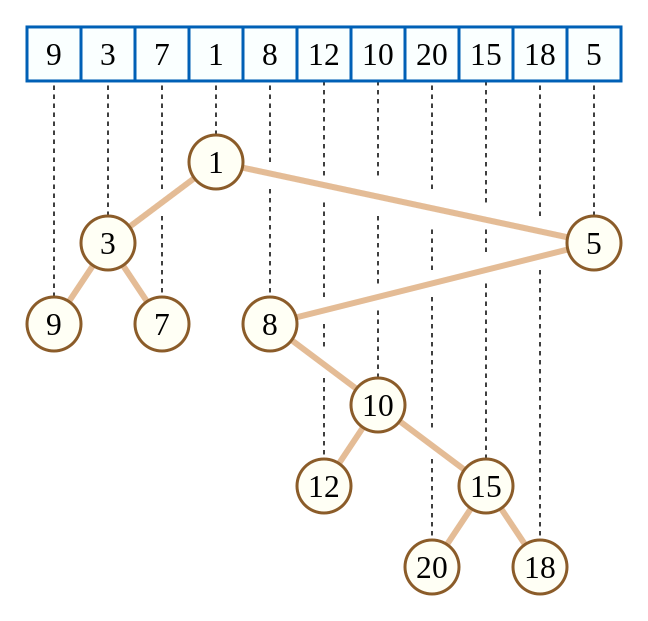
\includegraphics[width=5cm]{cartesian-tree1.png}
\end{center}
\begin{lstlisting}[style=cpp]
// cartesian tree //
vi ls(n + 1), rs(n + 1), stk(n + 1);
int top = 1;
for (int i = 1; i <= n; i++) {
    int k = top;
    while (k and a[stk[k]] > a[i]) k--;
    if (k) rs[stk[k]] = i;
    if (k < top) ls[i] = stk[k + 1];
    stk[++k] = i;
    top = k;
}
\end{lstlisting}

\subsection{ Treap }
$n$ 次操作, 操作分为如下 $6$ 种: 
\begin{itemize}
    \item 插入数 $x$
    \item 删除数 $x$( 若有多个相同的数, 只删除一个 )
    \item 查询数 $x$ 的排名( 排名定义为小于 $x$ 的数的个数 $+$ $1$ )
    \item 查询数 $x$ 的排名
    \item 求 $x$ 的前驱( 前驱定义为小于 $x$ 的最大数 )
    \item 求 $x$ 的后继( 后继定义为大于 $x$ 的最小数 )
\end{itemize}
\subsubsection{ 旋转 Treap }
\begin{lstlisting}[style=cpp]
// Problem: 洛谷: P3369 【模板】普通平衡树

int n, root, idx;

struct node {
    int l, r;
    int key, val;
    int cnt, size;
} treap[N];

void push_up(int p) {
    treap[p].size = treap[treap[p].l].size + treap[treap[p].r].size + treap[p].cnt;
}

int get_node(int key) {
    treap[++idx].key = key;
    treap[idx].val = rand();
    treap[idx].cnt = treap[idx].size = 1;
    return idx;
}

void zig(int &p) {
    // 右旋 //
    int q = treap[p].l;
    treap[p].l = treap[q].r, treap[q].r = p, p = q;
    push_up(treap[p].r), push_up(p);
}

void zag(int &p) {
    // 左旋 //
    int q = treap[p].r;
    treap[p].r = treap[q].l, treap[q].l = p, p = q;
    push_up(treap[p].l), push_up(p);
}

void build() {
    get_node(-inf), get_node(inf);
    root = 1, treap[1].r = 2;
    push_up(root);
    if (treap[1].val < treap[2].val) zag(root);
}

void insert(int &p, int key) {
    if (!p) {
        p = get_node(key);
    } else if (treap[p].key == key) {
        treap[p].cnt++;
    } else if (treap[p].key > key) {
        insert(treap[p].l, key);
        if (treap[treap[p].l].val > treap[p].val) zig(p);
    } else {
        insert(treap[p].r, key);
        if (treap[treap[p].r].val > treap[p].val) zag(p);
    }
    push_up(p);
}

void remove(int &p, int key) {
    if (!p) return;
    if (treap[p].key == key) {
        if (treap[p].cnt > 1) {
            treap[p].cnt--;
        } else if (treap[p].l || treap[p].r) {
            if (!treap[p].r || treap[treap[p].l].val > treap[treap[p].r].val) {
                zig(p);
                remove(treap[p].r, key);
            } else {
                zag(p);
                remove(treap[p].l, key);
            }
        } else {
            p = 0;
        }
    } else if {
        (treap[p].key > key) remove(treap[p].l, key);
    } else {
        remove(treap[p].r, key);
    }
    push_up(p);
}

int get_rank_by_key(int p, int key) {
    // 通过数值找排名 //
    if (!p) return 0;
    if (treap[p].key == key) return treap[treap[p].l].size;
    if (treap[p].key > key) return get_rank_by_key(treap[p].l, key);
    return treap[treap[p].l].size + treap[p].cnt + get_rank_by_key(treap[p].r, key);
}

int get_key_by_rank(int p, int rank) {
    // 通过排名找数值 //
    if (!p) return inf;
    if (treap[treap[p].l].size >= rank) return get_key_by_rank(treap[p].l, rank);
    if (treap[treap[p].l].size + treap[p].cnt >= rank) return treap[p].key;
    return get_key_by_rank(treap[p].r, rank - treap[treap[p].l].size - treap[p].cnt);
}

int get_prev(int p, int key) {
    // 找前驱 //
    if (!p) return -inf;
    if (treap[p].key >= key) return get_prev(treap[p].l, key);
    return max(treap[p].key, get_prev(treap[p].r, key));
}

int get_next(int p, int key) {
    // 找后继 //
    if (!p) return inf;
    if (treap[p].key <= key) return get_next(treap[p].r, key);
    return min(treap[p].key, get_next(treap[p].l, key));
}

int main() {
    ios::sync_with_stdio(false);
    cin.tie(0);
    cout.tie(0);

    cin >> n;
    build();
    rep(i, 1, n) {
        int op, x;
        cin >> op >> x;
        if (op == 1) {
            insert(root, x);
        } else if (op == 2) {
            remove(root, x);
        } else if (op == 3) {
            cout << get_rank_by_key(root, x) << endl;
        } else if (op == 4) {
            cout << get_key_by_rank(root, x + 1) << endl;
        } else if (op == 5) {
            cout << get_prev(root, x) << endl;
        } else {
            cout << get_next(root, x) << endl;
        }
    }
    return 0;
}
\end{lstlisting}

\subsubsection{ 无旋 Treap }
\begin{lstlisting}
// created on Laptop of Lucian Xu

struct node {
    node *ch[2];
    int key, val;
    int cnt, size;

    node(int _key) : key(_key), cnt(1), size(1) {
        ch[0] = ch[1] = nullptr;
        val = rand();
    }

    // node(node *_node) {
    // key = _node->key, val = _node->val, cnt = _node->cnt, size = _node->size;
    // }

    inline void push_up() {
        size = cnt;
        if (ch[0] != nullptr) size += ch[0]->size;
        if (ch[1] != nullptr) size += ch[1]->size;
    }
};

struct treap {
#define _2 second.first
#define _3 second.second

    node *root;

    pair<node *, node *> split(node *p, int key) {
        if (p == nullptr) return {nullptr, nullptr};
        if (p->key <= key) {
            auto temp = split(p->ch[1], key);
            p->ch[1] = temp.first;
            p->push_up();
            return {p, temp.second};
        } else {
            auto temp = split(p->ch[0], key);
            p->ch[0] = temp.second;
            p->push_up();
            return {temp.first, p};
        }
    }

    pair<node *, pair<node *, node *> > split_by_rank(node *p, int rank) {
        if (p == nullptr) return {nullptr, {nullptr, nullptr}};
        int ls_size = p->ch[0] == nullptr ? 0 : p->ch[0]->size;
        if (rank <= ls_size) {
            auto temp = split_by_rank(p->ch[0], rank);
            p->ch[0] = temp._3;
            p->push_up();
            return {temp.first, {temp._2, p}};
        } else if (rank <= ls_size + p->cnt) {
            node *lt = p->ch[0];
            node *rt = p->ch[1];
            p->ch[0] = p->ch[1] = nullptr;
            return {lt, {p, rt}};
        } else {
            auto temp = split_by_rank(p->ch[1], rank - ls_size - p->cnt);
            p->ch[1] = temp.first;
            p->push_up();
            return {p, {temp._2, temp._3}};
        }
    }

    node *merge(node *u, node *v) {
        if (u == nullptr && v == nullptr) return nullptr;
        if (u != nullptr && v == nullptr) return u;
        if (v != nullptr && u == nullptr) return v;
        if (u->val < v->val) {
            u->ch[1] = merge(u->ch[1], v);
            u->push_up();
            return u;
        } else {
            v->ch[0] = merge(u, v->ch[0]);
            v->push_up();
            return v;
        }
    }

    void insert(int key) {
        auto temp = split(root, key);
        auto l_tr = split(temp.first, key - 1);
        node *new_node;
        if (l_tr.second == nullptr) {
            new_node = new node(key);
        } else {
            l_tr.second->cnt++;
            l_tr.second->push_up();
        }
        node *l_tr_combined = merge(l_tr.first, l_tr.second == nullptr ? new_node : l_tr.second);
        root = merge(l_tr_combined, temp.second);
    }

    void remove(int key) {
        auto temp = split(root, key);
        auto l_tr = split(temp.first, key - 1);
        if (l_tr.second->cnt > 1) {
            l_tr.second->cnt--;
            l_tr.second->push_up();
            l_tr.first = merge(l_tr.first, l_tr.second);
        } else {
            if (temp.first == l_tr.second) temp.first = nullptr;
            delete l_tr.second;
            l_tr.second = nullptr;
        }
        root = merge(l_tr.first, temp.second);
    }

    int get_rank_by_key(node *p, int key) {
        auto temp = split(p, key - 1);
        int ret = (temp.first == nullptr ? 0 : temp.first->size) + 1;
        root = merge(temp.first, temp.second);
        return ret;
    }

    int get_key_by_rank(node *p, int rank) {
        auto temp = split_by_rank(p, rank);
        int ret = temp._2->key;
        root = merge(temp.first, merge(temp._2, temp._3));
        return ret;
    }

    int get_prev(int key) {
        auto temp = split(root, key - 1);
        int ret = get_key_by_rank(temp.first, temp.first->size);
        root = merge(temp.first, temp.second);
        return ret;
    }

    int get_nex(int key) {
        auto temp = split(root, key);
        int ret = get_key_by_rank(temp.second, 1);
        root = merge(temp.first, temp.second);
        return ret;
    }
};

treap tr;

int main() {
    ios::sync_with_stdio(false);
    cin.tie(0);
    cout.tie(0);

    srand(time(0));

    int n;
    cin >> n;
    while (n--) {
        int op, x;
        cin >> op >> x;
        if (op == 1) {
            tr.insert(x);
        } else if (op == 2) {
            tr.remove(x);
        } else if (op == 3) {
            cout << tr.get_rank_by_key(tr.root, x) << endl;
        } else if (op == 4) {
            cout << tr.get_key_by_rank(tr.root, x) << endl;
        } else if (op == 5) {
            cout << tr.get_prev(x) << endl;
        } else {
            cout << tr.get_nex(x) << endl;
        }
    }
    return 0;
}
\end{lstlisting}

\subsubsection{ 用 01 Trie 实现 }
使用 01 Trie 只能存在非负数. 

速度能快不少, 但只能单点操作, 而且有点费空间. 

\begin{lstlisting}[style=cpp]
// 洛谷 P3369 【模板】普通平衡树

struct Treap {
    int id = 1, maxlog = 25;
    int ch[N * 25][2], siz[N * 25];

    int newnode() {
        id++;
        ch[id][0] = ch[id][1] = siz[id] = 0;
        return id;
    }

    void merge(int key, int cnt) {
        int u = 1;
        for (int i = maxlog - 1; i >= 0; i--) {
            int v = (key >> i) & 1;
            if (!ch[u][v]) ch[u][v] = newnode();
            u = ch[u][v];
            siz[u] += cnt;
        }
    }

    int get_key_by_rank(int rank) {
        int u = 1, key = 0;
        for (int i = maxlog - 1; i >= 0; i--) {
            if (siz[ch[u][0]] >= rank) {
                u = ch[u][0];
            } else {
                key |= (1 << i);
                rank -= siz[ch[u][0]];
                u = ch[u][1];
            }
        }
        return key;
    }

    int get_rank_by_key(int rank) {
        int key = 0;
        int u = 1;
        for (int i = maxlog - 1; i >= 0; i--) {
            if ((rank >> i) & 1) {
                key += siz[ch[u][0]];
                u = ch[u][1];
            } else {
                u = ch[u][0];
            }
            if (!u) break;
        }
        return key;
    }

    int get_prev(int x) { return get_key_by_rank(get_rank_by_key(x)); }
    int get_next(int x) { return get_key_by_rank(get_rank_by_key(x + 1) + 1); }
} treap;

const int num = 1e7;
int n, op, x;

int main() {
    std::ios::sync_with_stdio(false);
    std::cin.tie(0);
    std::cout.tie(0);

    std::cin >> n;
    for (int i = 1; i <= n; i++) {
        std::cin >> op >> x;
        if (op == 1) {
            treap.merge(x + num, 1);
        } else if (op == 2) {
            treap.merge(x + num, -1);
        } else if (op == 3) {
            std::cout << treap.get_rank_by_key(x + num) + 1 << endl;
        } else if (op == 4) {
            std::cout << treap.get_key_by_rank(x) - num << endl;
        } else if (op == 5) {
            std::cout << treap.get_prev(x + num) - num << endl;
        } else if (op == 6) {
            std::cout << treap.get_next(x + num) - num << endl;
        }
    }
    return 0;
}
\end{lstlisting}

\subsection{ Splay }
\subsubsection{ 文艺平衡树 }
初始为 $1$ 到 $n$ 的序列, $m$ 次操作, 每次将序列下标为 $[l \sim r]$ 的区间翻转. 
\begin{lstlisting}
// 洛谷 P3391 【模板】文艺平衡树

struct node {
    int ch[2], fa, key;
    int siz, flag;

    void init(int _fa, int _key) { fa = _fa, key = _key, siz = 1; }
};

struct splay {
    node tr[N];
    int n, root, idx;

    bool get(int u) { return u == tr[tr[u].fa].ch[1]; }

    void pushup(int u) { tr[u].siz = tr[tr[u].ch[0]].siz + tr[tr[u].ch[1]].siz + 1; }

    void pushdown(int u) {
        if (tr[u].flag) {
            std::swap(tr[u].ch[0], tr[u].ch[1]);
            tr[tr[u].ch[0]].flag ^= 1, tr[tr[u].ch[1]].flag ^= 1;
            tr[u].flag = 0;
        }
    }

    void rotate(int x) {
        int y = tr[x].fa, z = tr[y].fa;
        int op = get(x);
        tr[y].ch[op] = tr[x].ch[op ^ 1];
        if (tr[x].ch[op ^ 1]) tr[tr[x].ch[op ^ 1]].fa = y;
        tr[x].ch[op ^ 1] = y;
        tr[y].fa = x, tr[x].fa = z;
        if (z) tr[z].ch[y == tr[z].ch[1]] = x;
        pushup(y), pushup(x);
    }

    void opt(int u, int k) {
        for (int f = tr[u].fa; f = tr[u].fa, f != k; rotate(u)) {
            if (tr[f].fa != k) rotate(get(u) == get(f) ? f : u);
        }
        if (k == 0) root = u;
    }

    void output(int u) {
        pushdown(u);
        if (tr[u].ch[0]) output(tr[u].ch[0]);
        if (tr[u].key >= 1 && tr[u].key <= n) {
            std::cout << tr[u].key << ' ';
        }
        if (tr[u].ch[1]) output(tr[u].ch[1]);
    }

    void insert(int key) {
        idx++;
        tr[idx].ch[0] = root;
        tr[idx].init(0, key);
        tr[root].fa = idx;
        root = idx;
        pushup(idx);
    }

    int kth(int k) {
        int u = root;
        while (1) {
            pushdown(u);
            if (tr[u].ch[0] && k <= tr[tr[u].ch[0]].siz) {
                u = tr[u].ch[0];
            } else {
                k -= tr[tr[u].ch[0]].siz + 1;
                if (k <= 0) {
                    opt(u, 0);
                    return u;
                } else {
                    u = tr[u].ch[1];
                }
            }
        }
    }

} splay;

int n, m, l, r;

int main() {
    std::ios::sync_with_stdio(false);
    std::cin.tie(0);
    std::cout.tie(0);

    std::cin >> n >> m;
    splay.n = n;
    splay.insert(-inf);
    rep(i, 1, n) splay.insert(i);
    splay.insert(inf);
    rep(i, 1, m) {
        std::cin >> l >> r;
        l = splay.kth(l), r = splay.kth(r + 2);
        splay.opt(l, 0), splay.opt(r, l);
        splay.tr[splay.tr[r].ch[0]].flag ^= 1;
    }
    splay.output(splay.root);

    return 0;
}
\end{lstlisting}

\subsubsection{ 普通平衡树 }
$n$ 次操作, 操作分为如下 $6$ 种: 
\begin{itemize}
 	\item 插入数 $x$
 	\item 删除数 $x$( 若有多个相同的数, 只删除一个 )
 	\item 查询数 $x$ 的排名( 排名定义为小于 $x$ 的数的个数 $+$ $1$ )
 	\item 查询排名为 $x$ 的数
 	\item 求 $x$ 的前驱( 前驱定义为小于 $x$ 的最大数 )
 	\item 求 $x$ 的后继( 后继定义为大于 $x$ 的最小数 )
\end{itemize}
\begin{lstlisting}
// 洛谷 P3369 【模板】普通平衡树

struct node {
    int ch[2], fa, key, siz, cnt;

    void init(int _fa, int _key) { fa = _fa, key = _key, siz = cnt = 1; }

    void clear() { ch[0] = ch[1] = fa = key = siz = cnt = 0; }
};

struct splay {
    node tr[N];
    int n, root, idx;

    bool get(int u) { return u == tr[tr[u].fa].ch[1]; }

    void pushup(int u) { tr[u].siz = tr[tr[u].ch[0]].siz + tr[tr[u].ch[1]].siz + tr[u].cnt; }

    void rotate(int x) {
        int y = tr[x].fa, z = tr[y].fa;
        int op = get(x);
        tr[y].ch[op] = tr[x].ch[op ^ 1];
        if (tr[x].ch[op ^ 1]) tr[tr[x].ch[op ^ 1]].fa = y;
        tr[x].ch[op ^ 1] = y;
        tr[y].fa = x, tr[x].fa = z;
        if (z) tr[z].ch[y == tr[z].ch[1]] = x;
        pushup(y), pushup(x);
    }

    void opt(int u, int k) {
        for (int f = tr[u].fa; f = tr[u].fa, f != k; rotate(u)) {
            if (tr[f].fa != k) {
                rotate(get(u) == get(f) ? f : u);
            }
        }
        if (k == 0) root = u;
    }

    void insert(int key) {
        if (!root) {
            idx++;
            tr[idx].init(0, key);
            root = idx;
            return;
        }
        int u = root, f = 0;
        while (1) {
            if (tr[u].key == key) {
                tr[u].cnt++;
                pushup(u), pushup(f);
                opt(u, 0);
                break;
            }
            f = u, u = tr[u].ch[tr[u].key < key];
            if (!u) {
                idx++;
                tr[idx].init(f, key);
                tr[f].ch[tr[f].key < key] = idx;
                pushup(idx), pushup(f);
                opt(idx, 0);
                break;
            }
        }
    }

    // 返回节点编号 //
    int kth(int rank) {
        int u = root;
        while (1) {
            if (tr[u].ch[0] && rank <= tr[tr[u].ch[0]].siz) {
                u = tr[u].ch[0];
            } else {
                rank -= tr[tr[u].ch[0]].siz + tr[u].cnt;
                if (rank <= 0) {
                    opt(u, 0);
                    return u;
                } else {
                    u = tr[u].ch[1];
                }
            }
        }
    }

    // 返回排名 //
    int nlt(int key) {
        int rank = 0, u = root;
        while (1) {
            if (tr[u].key > key) {
                u = tr[u].ch[0];
            } else {
                rank += tr[tr[u].ch[0]].siz;
                if (tr[u].key == key) {
                    opt(u, 0);
                    return rank + 1;
                }
                rank += tr[u].cnt;
                if (tr[u].ch[1]) {
                    u = tr[u].ch[1];
                } else {
                    return rank + 1;
                }
            }
        }
    }

    int get_prev(int key) { return kth(nlt(key) - 1); }

    int get_next(int key) { return kth(nlt(key + 1)); }

    void remove(int key) {
        nlt(key);
        if (tr[root].cnt > 1) {
            tr[root].cnt--;
            pushup(root);
            return;
        }
        int u = root, l = get_prev(key);
        tr[tr[u].ch[1]].fa = l;
        tr[l].ch[1] = tr[u].ch[1];
        tr[u].clear();
        pushup(root);
    }

    void output(int u) {
        if (tr[u].ch[0]) output(tr[u].ch[0]);
        std::cout << tr[u].key << ' ';
        if (tr[u].ch[1]) output(tr[u].ch[1]);
    }

} splay;

int n, op, x;

int main() {
    std::ios::sync_with_stdio(false);
    std::cin.tie(0);
    std::cout.tie(0);

    splay.insert(-inf), splay.insert(inf);

    std::cin >> n;
    for (int i = 1; i <= n; i++) {
        std::cin >> op >> x;
        if (op == 1) {
            splay.insert(x);
        } else if (op == 2) {
            splay.remove(x);
        } else if (op == 3) {
            std::cout << splay.nlt(x) - 1 << endl;
        } else if (op == 4) {
            std::cout << splay.tr[splay.kth(x + 1)].key << endl;
        } else if (op == 5) {
            std::cout << splay.tr[splay.get_prev(x)].key << endl;
        } else if (op == 6) {
            std::cout << splay.tr[splay.get_next(x)].key << endl;
        }
    }

    return 0;
}
\end{lstlisting}

\subsection{ 树套树 }
\subsubsection{ 线段树套线段树 }
$n$ 个三维数对 $(a_i, b_i, c_i)$, 设 $f(i)$ 表示 $a_j \leqslant a_i$ 且 $b_j \leqslant b_i$ 且  $c_j \leqslant c_i$ 且 $i \neq j$ 的个数. 

输出 $f(i) \ (0 \leqslant i \leqslant n - 1)$ 的值. 
\begin{lstlisting}
// 洛谷 P3810 【模板】三维偏序( 陌上花开 )

struct node1 {
    int l, r, root;
} tr1[N << 2];

struct node2 {
    int ch[2], cnt;
} tr2[N << 7];

struct node {
    int x, y, z, cnt;

    bool operator==(const node& a) { return (x == a.x && y == a.y && z == a.z); }

} data[N];

bool cmp(node a, node b) {
    if (a.x != b.x) return a.x < b.x;
    if (a.y != b.y) return a.y < b.y;
    return a.z < b.z;
}

int root_tot, n, m, ans[N], anss[N];

void build(int u, int l, int r) {
    tr1[u].l = l, tr1[u].r = r;
    if (l != r) {
        int mid = (l + r) >> 1;
        build(u << 1, l, mid);
        build(u << 1 | 1, mid + 1, r);
    }
}

void modify_2(int& u, int l, int r, int pos) {
    if (u == 0) u = ++root_tot;
    tr2[u].cnt++;
    if (l == r) return;
    int mid = (l + r) >> 1;
    if (pos <= mid) {
        modify_2(tr2[u].ch[0], l, mid, pos);
    } else {
        modify_2(tr2[u].ch[1], mid + 1, r, pos);
    }
}

int query_2(int& u, int l, int r, int x, int y) {
    if (u == 0) return 0;
    if (x <= l && r <= y) return tr2[u].cnt;
    int mid = (l + r) >> 1, ans = 0;
    if (x <= mid) ans += query_2(tr2[u].ch[0], l, mid, x, y);
    if (mid < y) ans += query_2(tr2[u].ch[1], mid + 1, r, x, y);
    return ans;
}

void modify_1(int u, int l, int r, int t) {
    modify_2(tr1[u].root, 1, m, data[t].z);
    if (l == r) return;
    int mid = (l + r) >> 1;
    if (data[t].y <= mid) {
        modify_1(u << 1, l, mid, t);
    } else {
        modify_1(u << 1 | 1, mid + 1, r, t);
    }
}

int query_1(int u, int l, int r, int t) {
    if (1 <= l && r <= data[t].y) return query_2(tr1[u].root, 1, m, 1, data[t].z);
    int mid = (l + r) >> 1, ans = 0;
    if (1 <= mid) ans += query_1(u << 1, l, mid, t);
    if (mid < data[t].y) ans += query_1(u << 1 | 1, mid + 1, r, t);
    return ans;
}

int main() {
    std::ios::sync_with_stdio(false);
    std::cin.tie(0);
    std::cout.tie(0);

    std::cin >> n >> m;
    rep(i, 1, n) {
        int x, y, z;
        std::cin >> x >> y >> z;
        data[i] = {x, y, z};
    }
    std::sort(data + 1, data + n + 1, cmp);
    build(1, 1, m);
    rep(i, 1, n) {
        modify_1(1, 1, m, i);
        ans[i] = query_1(1, 1, m, i);
    }
    per(i, n - 1, 1) {
        if (data[i] == data[i + 1]) ans[i] = ans[i + 1];
    }
    rep(i, 1, n) anss[ans[i]]++;
    rep(i, 1, n) std::cout << anss[i] << endl;

    return 0;
}
\end{lstlisting}

\subsubsection{ 线段树套平衡树 }
长度为 $n$ 的序列和 $m$ 此操作, 包含 $5$ 种操作: 
\begin{itemize}
	\item $l \ r \ k$: 询问区间 $[l \sim r]$ 中数 $k$ 的排名. 
	\item $l \ r \ k$: 询问区间 $[l \sim r]$ 中排名为 $k$ 的数. 
	\item $pos \ k$: 将序列中 $pos$ 位置的数修改为 $k$ . 
	\item $l \ r \ k$: 询问区间 $[l \sim r]$ 中数 $k$ 的前驱. 
	\item $l \ r \ k$: 询问区间 $[l \sim r]$ 中数 $k$ 的后继. 
\end{itemize}
Treap 实现
\begin{lstlisting}
// 洛谷 P3380 【模板】二逼平衡树( 树套树 )

int n, m, op, l, r, pos, key, root_tot;
int a[N];

struct node2 {
    node2 *ch[2];
    int key, val;
    int cnt, size;

    node2(int _key) : key(_key), cnt(1), size(1) {
        ch[0] = ch[1] = nullptr;
        val = rand();
    }

    // node2(node2 *_node2) {
    // key = _node2->key, val = _node2->val, cnt = _node2->cnt, size = _node2->size;
    // }

    inline void push_up() {
        size = cnt;
        if (ch[0] != nullptr) size += ch[0]->size;
        if (ch[1] != nullptr) size += ch[1]->size;
    }
};

struct treap {
    ···
};

treap tr2[N << 4];

struct node1 {
    int l, r, root;
} tr1[N << 4];

void build(int u, int l, int r) {
    tr1[u] = {l, r, u};
    root_tot = std::max(root_tot, u);
    if (l == r) return;
    int mid = (l + r) >> 1;
    build(u << 1, l, mid), build(u << 1 | 1, mid + 1, r);
}

void modify(int u, int pos, int key) {
    tr2[u].insert(key);
    if (tr1[u].l == tr1[u].r) return;
    int mid = (tr1[u].l + tr1[u].r) >> 1;
    if (pos <= mid){
        modify(u << 1, pos, key);
    }
    else{
        modify(u << 1 | 1, pos, key);
    }
}

int get_rank_by_key_in_interval(int u, int l, int r, int key) {
    if (l <= tr1[u].l && tr1[u].r <= r) return tr2[u].get_rank_by_key(tr2[u].root, key) - 2;
    int mid = (tr1[u].l + tr1[u].r) >> 1, ans = 0;
    if (l <= mid) ans += get_rank_by_key_in_interval(u << 1, l, r, key);
    if (mid < r) ans += get_rank_by_key_in_interval(u << 1 | 1, l, r, key);
    return ans;
}

int get_key_by_rank_in_interval(int u, int l, int r, int rank) {
    int L = 0, R = 1e8;
    while (L < R) {
        int mid = (L + R + 1) / 2;
        if (get_rank_by_key_in_interval(1, l, r, mid) < rank){
            L = mid;
        }
        else{
            R = mid - 1;
        }
    }
    return L;
}

void change(int u, int pos, int pre_key, int key) {
    tr2[u].remove(pre_key);
    tr2[u].insert(key);
    if (tr1[u].l == tr1[u].r) return;
    int mid = (tr1[u].l + tr1[u].r) >> 1;
    if (pos <= mid){
        change(u << 1, pos, pre_key, key);
    }
    else{
        change(u << 1 | 1, pos, pre_key, key);
    }
}

int get_prev_in_interval(int u, int l, int r, int key) {
    if (l <= tr1[u].l && tr1[u].r <= r) return tr2[u].get_prev(key);
    int mid = (tr1[u].l + tr1[u].r) >> 1, ans = -inf;
    if (l <= mid) ans = std::max(ans, get_prev_in_interval(u << 1, l, r, key));
    if (mid < r) ans = std::max(ans, get_prev_in_interval(u << 1 | 1, l, r, key));
    return ans;
}

int get_nex_in_interval(int u, int l, int r, int key) {
    if (l <= tr1[u].l && tr1[u].r <= r) return tr2[u].get_nex(key);
    int mid = (tr1[u].l + tr1[u].r) >> 1, ans = inf;
    if (l <= mid) ans = std::min(ans, get_nex_in_interval(u << 1, l, r, key));
    if (mid < r) ans = std::min(ans, get_nex_in_interval(u << 1 | 1, l, r, key));
    return ans;
}

int main() {
    std::ios::sync_with_stdio(false);
    std::cin.tie(0);
    std::cout.tie(0);

    srand(time(0));

    std::cin >> n >> m;
    build(1, 1, n);
    rep(i, 1, n) {
        std::cin >> a[i];
        modify(1, i, a[i]);
    }
    rep(i, 1, root_tot) { tr2[i].insert(inf), tr2[i].insert(-inf); }
    rep(i, 1, m) {
        std::cin >> op;
        if (op == 1) {
            std::cin >> l >> r >> key;
            std::cout << get_rank_by_key_in_interval(1, l, r, key) + 1 << endl;
        } else if (op == 2) {
            std::cin >> l >> r >> key;
            std::cout << get_key_by_rank_in_interval(1, l, r, key) << endl;
        } else if (op == 3) {
            std::cin >> pos >> key;
            change(1, pos, a[pos], key);
            a[pos] = key;
        } else if (op == 4) {
            std::cin >> l >> r >> key;
            std::cout << get_prev_in_interval(1, l, r, key) << endl;
        } else if (op == 5) {
            std::cin >> l >> r >> key;
            std::cout << get_nex_in_interval(1, l, r, key) << endl;
        
    }

    return 0;
}
\end{lstlisting}
然而洛谷上的会 T 两个点, Loj 和 ACwing 上的能过. 

Splay 实现
\begin{lstlisting}
// 洛谷 P3380 【模板】二逼平衡树( 树套树 )

int n, m, op, l, r, pos, key, root_tot;
int a[N];

struct node{
    int ch[2], fa, key, siz, cnt;
    
    void init(int _fa, int _key){
        fa = _fa, key = _key, siz = cnt = 1;
    }
    
    void clear(){
        ch[0] = ch[1] = fa = key = siz = cnt = 0;
    }
}tr[N * 30];

struct splay{
    
    int idx;
    
    bool get(int u){
        return u == tr[tr[u].fa].ch[1];
    }
    
    void pushup(int u){
        tr[u].siz = tr[tr[u].ch[0]].siz + tr[tr[u].ch[1]].siz + tr[u].cnt;
    }
    
    void rotate(int x){
        int y = tr[x].fa, z = tr[y].fa;
        int op = get(x);
        tr[y].ch[op] = tr[x].ch[op ^ 1];
        if(tr[x].ch[op ^ 1]) tr[tr[x].ch[op ^ 1]].fa = y;
        tr[x].ch[op ^ 1] = y;
        tr[y].fa = x, tr[x].fa = z;
        if(z) tr[z].ch[y == tr[z].ch[1]] = x;
        pushup(y), pushup(x);
    }
    
    void opt(int& root, int u, int k){
        for(int f = tr[u].fa; f = tr[u].fa, f != k; rotate(u)){
            if(tr[f].fa != k) rotate(get(u) == get(f) ? f : u);
        }
        if(k == 0) root = u;
    }
    
    void insert(int& root, int key){
        if(tr[root].siz == 0){
            idx++;
            tr[idx].init(0, key);
            root = idx;
            return;
        }
        int u = root, f = 0;
        while(1){
            if(tr[u].key == key){
                tr[u].cnt++;
                pushup(u), pushup(f);
                opt(root, u, 0);
                break;
            }
            f = u, u = tr[u].ch[tr[u].key < key];
            if(!u){
                idx++;
                tr[idx].init(f, key);
                tr[f].ch[tr[f].key < key] = idx;
                pushup(idx), pushup(f);
                opt(root, idx, 0);
                break;
            }
        }
    }
    
    int kth(int& root, int rank){
        int u = root;
        while(1){
            if(tr[u].ch[0] && rank <= tr[tr[u].ch[0]].siz) u = tr[u].ch[0];
            else{
                rank -= tr[tr[u].ch[0]].siz + tr[u].cnt;
                if(rank <= 0){
                    opt(root, u, 0);
                    return u;
                }
                else u = tr[u].ch[1];
            }
        }
    }
    
    int nlt(int& root, int key){
        int rank = 0, u = root;
        while(1){
            if(tr[u].key > key) u = tr[u].ch[0];
            else{
                rank += tr[tr[u].ch[0]].siz;
                if(tr[u].key == key){
                    opt(root, u, 0);
                    return rank + 1;
                }
                rank += tr[u].cnt;
                if(tr[u].ch[1]) u = tr[u].ch[1];
                else return rank + 1;
            }
        }
    }
    
    int get_prev(int& root, int key){
        return kth(root, nlt(root, key) - 1);
    }
    
    int get_next(int& root, int key){
        return kth(root, nlt(root, key + 1));
    }
    
    void remove(int& root, int key){
        nlt(root, key);
        if(tr[root].cnt > 1){
            tr[root].cnt--;
            pushup(root);
            return;
        }
        int u = root, l = get_prev(root, key);
        tr[tr[u].ch[1]].fa = l;
        tr[l].ch[1] = tr[u].ch[1];
        tr[u].clear();
        pushup(root);
    }
    
    void output(int u){
        if(tr[u].ch[0]) output(tr[u].ch[0]);
        std::cout << tr[u].key << ' ';
        if(tr[u].ch[1]) output(tr[u].ch[1]);
    }
    
}splay;

struct node1{
    int l, r, root;
}tr1[N * 4];

void build(int u, int l, int r){
    tr1[u] = {l, r, u};
    root_tot = splay.idx = std::max(root_tot, u);
    if(l == r) return;
    int mid = (l + r) >> 1;
    build(u << 1, l, mid), build(u << 1 | 1, mid + 1, r);
}

void modify(int u, int pos, int key){
    splay.insert(tr1[u].root, key);
    if(tr1[u].l == tr1[u].r) return;
    int mid = (tr1[u].l + tr1[u].r) >> 1;
    if(pos <= mid) modify(u << 1, pos, key);
    else modify(u << 1 | 1, pos, key);
}

int get_rank_by_key_in_interval(int u, int l, int r, int key){
    if(l <= tr1[u].l && tr1[u].r <= r) 
        return splay.nlt(tr1[u].root, key) - 2;
    int mid = (tr1[u].l + tr1[u].r) >> 1, ans = 0;
    if(l <= mid) ans += get_rank_by_key_in_interval(u << 1, l, r, key);
    if(mid < r) ans += get_rank_by_key_in_interval(u << 1 | 1, l, r, key);
    return ans;
}

int get_key_by_rank_in_interval(int u, int l, int r, int rank){
    int L = 0, R = 1e8;
    while(L < R){
        int mid = (L + R + 1) / 2;
        if(get_rank_by_key_in_interval(1, l, r, mid) < rank) L = mid;
        else R = mid - 1;
    }
    return L;
}

void change(int u, int pos, int pre_key, int key){
    splay.remove(tr1[u].root, pre_key);
    splay.insert(tr1[u].root, key);
    if(tr1[u].l == tr1[u].r) return;
    int mid = (tr1[u].l + tr1[u].r) >> 1;
    if(pos <= mid) change(u << 1, pos, pre_key, key);
    else change(u << 1 | 1, pos, pre_key, key);
}

int get_prev_in_interval(int u, int l, int r, int key){
    if(l <= tr1[u].l && tr1[u].r <= r)
        return tr[splay.get_prev(tr1[u].root, key)].key;
    int mid = (tr1[u].l + tr1[u].r) >> 1, ans = -inf;
    if(l <= mid) ans = std::max(ans, get_prev_in_interval(u << 1, l, r, key));
    if(mid < r) ans = std::max(ans, get_prev_in_interval(u << 1 | 1, l, r, key));
    return ans;
        
}

int get_next_in_interval(int u, int l, int r, int key){
    if(l <= tr1[u].l && tr1[u].r <= r)
        return tr[splay.get_next(tr1[u].root, key)].key;
    int mid = (tr1[u].l + tr1[u].r) >> 1, ans = inf;
    if(l <= mid) ans = std::min(ans, get_next_in_interval(u << 1, l, r, key));
    if(mid < r) ans = std::min(ans, get_next_in_interval(u << 1 | 1, l, r, key));
    return ans;
}

int main(){
    
    std::ios::sync_with_stdio(false);
    std::cin.tie(0);
    std::cout.tie(0);
    
    srand(time(0));
    
    std::cin >> n >> m;
    build(1, 1, n);
    rep(i, 1, n){
        std::cin >> a[i];
        modify(1, i, a[i]);
    }
    rep(i, 1, root_tot){
        splay.insert(tr1[i].root, inf), splay.insert(tr1[i].root, -inf); 
    }
    rep(i, 1, m){
        std::cin >> op;
        if(op == 1){
            std::cin >> l >> r >> key;
            std::cout << get_rank_by_key_in_interval(1, l, r, key) + 1 << endl;
        }
        else if(op == 2){
            std::cin >> l >> r >> key;
            std::cout << get_key_by_rank_in_interval(1, l, r, key) << endl;
        }
        else if(op == 3){
            std::cin >> pos >> key;
            change(1, pos, a[pos], key);
            a[pos] = key;
        }
        else if(op == 4){
            std::cin >> l >> r >> key;
            std::cout << get_prev_in_interval(1, l, r, key) << endl;
        }
        else if(op == 5){
            std::cin >> l >> r >> key;
            std::cout << get_next_in_interval(1, l, r, key) << endl;
        }
    }
    
    return 0;
}
\end{lstlisting}
然而洛谷吸氧能过, ACwing能过, Loj T一堆. 

\newpage
\section{ 字符串 }

\subsection{ 字典树 }
\subsubsection{ 普通字典树 (单词匹配) }
\begin{lstlisting}

// trie //
int cnt;
std::vector<std::array<int, 26>> trie(n + 1);
vi exist(n + 1);

auto insert = [&](string s) -> void {
    int p = 0;
    for (int i = 0; i < s.size() - 1; i++) {
        int c = s[i] - 'a';
        if (!trie[p][c]) trie[p][c] = ++cnt;
        p = trie[p][c];
    }
    exist[p] = true;
};

auto find = [&](string s) -> bool {
    int p = 0;
    for (int i = 0; i < s.size() - 1; i++) {
        int c = s[i] - 'a';
        if (!trie[p][c]) return false;
        p = trie[p][c];
    }
    return exist[p];
};
\end{lstlisting}

\subsubsection{ 01字典树( 求最大异或值 ) }
给定 $n$ 个数, 取两个数进行异或运算, 求最大异或值. 
\begin{lstlisting}
// trie //
int cnt = 0;
std::vector<std::array<int, 2>> trie(N);

auto insert = [&](int x) -> void {
    int p = 0;
    for (int i = 30; i >= 0; i--) {
        int c = (x >> i) & 1;
        if (!trie[p][c]) trie[p][c] = ++cnt;
        p = trie[p][c];
    }
};

auto find = [&](int x) -> int {
    int sum = 0, p = 0;
    for (int i = 30; i >= 0; i--) {
        int c = (x >> i) & 1;
        if (trie[p][c ^ 1]) {
            p = trie[p][c ^ 1];
            sum += (1 << i);
        } else {
            p = trie[p][c];
        }
    }
    return sum;
};
\end{lstlisting}

\subsubsection{ 字典树合并 }
来自浙大城市学院 2023 校赛 E 题. 

给定一棵根为 $1$ 的树, 每个点的点权为 $w_i$. 一共 $q$ 次询问, 每次给出一对 $u$, $v$, 询问以 $v$ 为根的子树上的点与 $u$ 的权值最大异或值. 
\begin{lstlisting}
int main() {
    std::ios::sync_with_stdio(false);
    std::cin.tie(0);
    std::cout.tie(0);

    int n, m;
    std::cin >> n;
    vi w(n + 1);
    for (int i = 1; i <= n; i++) {
        std::cin >> w[i];
    }

    vvi e(n + 1);
    for (int i = 1; i < n; i++) {
        int u, v;
        std::cin >> u >> v;
        e[u].push_back(v);
        e[v].push_back(u);
    }

    // 离线询问 //
    std::cin >> m;
    std::vector<vpi> q(n + 1);
    vi ans(m + 1);
    for (int i = 1; i <= m; i++) {
        int u, v;
        std::cin >> u >> v;
        q[v].emplace_back(u, i);
    }

    // 01 trie //
    std::vector<std::array<int, 2>> tr(1);

    auto new_node = [&]() -> int {
        tr.emplace_back();
        return tr.size() - 1;
    };

    vi id(n + 1);

    auto insert = [&](int root, int x) {
        int p = root;
        for (int i = 29; i >= 0; i--) {
            int c = x >> i & 1;
            if (!tr[p][c]) tr[p][c] = new_node();
            p = tr[p][c];
        }
    };

    auto query = [&](int root, int x) -> int {
        int ans = 0, p = root;
        for (int i = 29; i >= 0; i--) {
            int c = x >> i & 1;
            if (tr[p][c ^ 1]) {
                p = tr[p][c ^ 1];
                ans += (1 << i);
            } else {
                p = tr[p][c];
            }
        }
        return ans;
    };

    std::function<int(int, int)> merge = [&](int a, int b) -> int {
        // b 的信息挪到 a 上 //
        if (!a) return b;
        if (!b) return a;
        tr[a][0] = merge(tr[a][0], tr[b][0]);
        tr[a][1] = merge(tr[a][1], tr[b][1]);
        return a;
    };

    std::function<void(int, int)> dfs = [&](int u, int fa) {
        id[u] = new_node();
        insert(id[u], w[u]);
        for (auto v : e[u]) {
            if (v == fa) continue;
            dfs(v, u);
            id[u] = merge(id[u], id[v]);
        }
        for (auto [v, i] : q[u]) {
            ans[i] = query(id[u], w[v]);
        }
    };
    dfs(1, 0);

    for (int i = 1; i <= m; i++) std::cout << ans[i] << endl;

    return 0;
}
\end{lstlisting}

\subsection{ KMP }

这一节的 $string$ 都是从 $0$ 开始计数. 

\subsubsection{ 计算 $next$ 数组 }
\begin{lstlisting}
auto get_next = [&](string s) -> vi {
    int n = s.length();
    vi next(n);
    for (int i = 1; i < n; i++) {
        int j = next[i - 1];
        while (j > 0 and s[i] != s[j]) j = next[j - 1];
        if (s[i] == s[j]) j++;
        next[i] = j;
    }
    return next;
};
\end{lstlisting}

\subsubsection{ 在文本串中匹配模式串 }
求出 $s$ 在 $t$ 中所有出现的位置.

用脏字符连接文本串与模式串跑 KMP 即可.

\subsubsection{ 字符串的最小周期 }

如果周期大于 $1$, $n - next[n-1]$ 是最小周期.

如果周期为 $1$, 满足条件:

\begin{enumerate}
	\item $next[n-1] = n$;
	\item $next[n-1] \neq n$, 但计算出来的并不是循环节, 暴力判断一下.
\end{enumerate}

\subsection{ Z 函数 }

这一节的 $string$ 都是从 $0$ 开始计数. 

\subsubsection{ 计算 $z$ 数组 }
\begin{lstlisting}[style=cpp]
auto z_function = [&](const std::string& s) -> vi {
    int n = s.size();
    vi z(n);
    for (int i = 1, l = 0, r = 0; i < n; i++) {
        if (i <= r and z[i - l] < r - i + 1) {
            z[i] = z[i - l];
        } else {
            z[i] = std::max(0, r - i + 1);
            while (z[i] + i < n and s[z[i]] == s[z[i] + i]) z[i]++;
        }
        if (z[i] + i - 1 > r) {
            l = i;
            r = z[i] + i - 1;
        }
    }
    return z;
};
\end{lstlisting}

\newpage
\section{ 数学 - 多项式 }
\subsection{ FFT }
\begin{lstlisting}[style=cpp]
const int sz = 1 << 23;
int rev[sz];
int rev_n;
void set_rev(int n) {
    if (n == rev_n) return;
    for (int i = 0; i < n; i++) rev[i] = (rev[i / 2] | (i & 1) * n) / 2;
    rev_n = n;
}
tempt void butterfly(T* a, int n) {
    set_rev(n);
    for (int i = 0; i < n; i++) {
        if (i < rev[i]) std::swap(a[i], a[rev[i]]);
    }
}

namespace Comp {

long double pi = 3.141592653589793238;

tempt struct complex {
    T x, y;
    complex(T x = 0, T y = 0) : x(x), y(y) {}
    complex operator+(const complex& b) const { return complex(x + b.x, y + b.y); }

    complex operator-(const complex& b) const { return complex(x - b.x, y - b.y); }

    complex operator*(const complex& b) const {
        return complex<T>(x * b.x - y * b.y, x * b.y + y * b.x);
    }
    complex operator~() const { return complex(x, -y); }
    static complex unit(long double rad) { return complex(std::cos(rad), std::sin(rad)); }
};

}    // namespace Comp

struct fft_t {
    typedef Comp::complex<double> complex;
    complex wn[sz];

    fft_t() {
        for (int i = 0; i < sz / 2; i++) {
            wn[sz / 2 + i] = complex::unit(2 * Comp::pi * i / sz);
        }
        for (int i = sz / 2 - 1; i; i--) wn[i] = wn[i * 2];
    }

    void operator()(complex* a, int n, int type) {
        if (type == -1) std::reverse(a + 1, a + n);
        butterfly(a, n);
        for (int i = 1; i < n; i *= 2) {
            const complex* w = wn + i;
            for (complex *b = a, t; b != a + n; b += i + 1) {
                t = b[i];
                b[i] = *b - t;
                *b = *b + t;
                for (int j = 1; j < i; j++) {
                    t = (++b)[i] * w[j];
                    b[i] = *b - t;
                    *b = *b + t;
                }
            }
        }
        if (type == 1) return;
        for (int i = 0; i < n * 2; i++) ((double*) a)[i] /= n;
    }
} FFT;

typedef decltype(FFT)::complex complex;

\end{lstlisting}

\subsubsection{ FFT }
\begin{lstlisting}[style=cpp]
vi fft(const vi& f, const vi& g) {
    static complex ff[sz];
    int n = f.size(), m = g.size();
    vi h(n + m - 1);
    if (std::min(n, m) <= 50) {
        for (int i = 0; i < n; i++) {
            for (int j = 0; j < m; ++j) {
                h[i + j] += f[i] * g[j];
            }
        }
        return h;
    }
    int c = 1;
    while (c + 1 < n + m) c *= 2;
    std::memset(ff, 0, sizeof(decltype(*(ff))) * (c));
    for (int i = 0; i < n; i++) ff[i].x = f[i];
    for (int i = 0; i < m; i++) ff[i].y = g[i];
    FFT(ff, c, 1);
    for (int i = 0; i < c; i++) ff[i] = ff[i] * ff[i];
    FFT(ff, c, -1);
    for (int i = 0; i + 1 < n + m; i++) h[i] = std::llround(ff[i].y / 2);
    return h;
}
\end{lstlisting}

\subsubsection{ 拆系数FFT }
注意改头文件模板的 mod 数.
\begin{lstlisting}[style=cpp]
vi mtt(const vi& f, const vi& g) {
    static complex ff[3][sz], gg[2][sz];
    static int s[3] = {1, 31623, 31623 * 31623};
    int n = f.size(), m = g.size();
    vi h(n + m - 1);
    if (std::min(n, m) <= 50) {
        for (int i = 0; i < n; ++i) {
            for (int j = 0; j < m; ++j) {
                Add(h[i + j], mul(f[i], g[j]));
            }
        }
        return h;
    }
    int c = 1;
    while (c + 1 < n + m) c *= 2;
    for (int i = 0; i < 2; ++i) {
        std::memset(ff[i], 0, sizeof(decltype(*(ff[i]))) * (c));
        std::memset(gg[i], 0, sizeof(decltype(*(ff[i]))) * (c));
        for (int j = 0; j < n; ++j) ff[i][j].x = f[j] / s[i] % s[1];
        for (int j = 0; j < m; ++j) gg[i][j].x = g[j] / s[i] % s[1];
        FFT(ff[i], c, 1);
        FFT(gg[i], c, 1);
    }
    for (int i = 0; i < c; ++i) {
        ff[2][i] = ff[1][i] * gg[1][i];
        ff[1][i] = ff[1][i] * gg[0][i];
        gg[1][i] = ff[0][i] * gg[1][i];
        ff[0][i] = ff[0][i] * gg[0][i];
    }
    for (int i = 0; i < 3; ++i) {
        FFT(ff[i], c, -1);
        for (int j = 0; j + 1 < n + m; ++j) {
            Add(h[j], mul(std::llround(ff[i][j].x) % mod, s[i]));
        }
    }
    FFT(gg[1], c, -1);
    for (int i = 0; i + 1 < n + m; ++i) {
        Add(h[i], mul(std::llround(gg[1][i].x) % mod, s[1]));
    }
    return h;
}
\end{lstlisting}

\subsection{ NTT 全家桶 }
\begin{lstlisting}[style=cpp]
class polynomial : public vi {
   public:
    polynomial() = default;
    polynomial(const vi& v) : vi(v) {}
    polynomial(vi&& v) : vi(std::move(v)) {}

    int degree() { return size() - 1; }

    void clearzero() {
        while (size() && !back()) pop_back();
    }
};


polynomial& operator+=(polynomial& a, const polynomial& b) {
    a.resize(std::max(a.size(), b.size()), 0);
    for (int i = 0; i < b.size(); i++) {
        Add(a[i], b[i]);
    }
    a.clearzero();
    return a;
}

polynomial operator+(const polynomial& a, const polynomial& b) {
    polynomial ans = a;
    return ans += b;
}

polynomial& operator-=(polynomial& a, const polynomial& b) {
    a.resize(std::max(a.size(), b.size()), 0);
    for (int i = 0; i < b.size(); i++) {
        Sub(a[i], b[i]);
    }
    a.clearzero();
    return a;
}

polynomial operator-(const polynomial& a, const polynomial& b) {
    polynomial ans = a;
    return ans -= b;
}

class ntt_t {
   public:
    static const int maxbit = 22;
    static const int sz = 1 << maxbit;
    static const int mod = 998244353;
    static const int g = 3;

    std::array<int, sz + 10> w;
    std::array<int, maxbit + 10> len_inv;

    ntt_t() {
        int wn = pow(g, (mod - 1) >> maxbit);
        w[0] = 1;
        for (int i = 1; i <= sz; i++) {
            w[i] = mul(w[i - 1], wn);
        }
        len_inv[maxbit] = pow(sz, mod - 2);
        for (int i = maxbit - 1; ~i; i--) {
            len_inv[i] = add(len_inv[i + 1], len_inv[i + 1]);
        }
    }

    void operator()(vi& v, int& n, int type) {
        int bit = 0;
        while ((1 << bit) < n) bit++;
        int tot = (1 << bit);
        v.resize(tot, 0);
        vi rev(tot);
        n = tot;
        for (int i = 0; i < tot; i++) {
            rev[i] = rev[i >> 1] >> 1;
            if (i & 1) {
                rev[i] |= tot >> 1;
            }
        }
        for (int i = 0; i < tot; i++) {
            if (i < rev[i]) {
                std::swap(v[i], v[rev[i]]);
            }
        }
        for (int midd = 0; (1 << midd) < tot; midd++) {
            int mid = 1 << midd;
            int len = mid << 1;
            for (int i = 0; i < tot; i += len) {
                for (int j = 0; j < mid; j++) {
                    int w0 = v[i + j];
                    int w1 = mul(
                        w[type == 1 ? (j << maxbit - midd - 1) : (len - j << maxbit - midd - 1)],
                        v[i + j + mid]);
                    v[i + j] = add(w0, w1);
                    v[i + j + mid] = sub(w0, w1);
                }
            }
        }
        if (type == -1) {
            for (int i = 0; i < tot; i++) {
                v[i] = mul(v[i], len_inv[bit]);
            }
        }
    }
} NTT;
\end{lstlisting}

\subsubsection{ 乘法 }
\begin{lstlisting}[style=cpp]
polynomial& operator*=(polynomial& a, const polynomial& b) {
    if (!a.size() || !b.size()) {
        a.resize(0);
        return a;
    }
    polynomial tmp = b;
    int deg = a.size() + b.size() - 1;
    int temp = deg;

    // 项数较小直接硬算

    if ((LL) a.size() * (LL) b.size() <= (LL) deg * 50LL) {
        tmp.resize(0);
        tmp.resize(deg, 0);
        for (int i = 0; i < a.size(); i++) {
            for (int j = 0; j < b.size(); j++) {
                tmp[i + j] = add(tmp[i + j], mul(a[i], b[j]));
            }
        }
        a = tmp;
        return a;
    }

    // 项数较多跑 NTT

    NTT(a, deg, 1);
    NTT(tmp, deg, 1);
    for (int i = 0; i < deg; i++) {
        Mul(a[i], tmp[i]);
    }
    NTT(a, deg, -1);
    a.resize(temp);
    return a;
}

polynomial operator*(const polynomial& a, const polynomial& b) {
    polynomial ans = a;
    return ans *= b;
}
\end{lstlisting}

\subsubsection{ 逆 }
\begin{lstlisting}[style=cpp]
polynomial inverse(const polynomial& a) {
    polynomial ans({pow(a[0], mod - 2)});
    polynomial temp;
    polynomial tempa;
    int deg = a.size();
    for (int i = 0; (1 << i) < deg; i++) {
        tempa.resize(0);
        tempa.resize(1 << i << 1, 0);
        for (int j = 0; j != tempa.size() and j != deg; j++) {
            tempa[j] = a[j];
        }
        temp = ans * (polynomial({2}) - tempa * ans);
        if (temp.size() > (1 << i << 1)) {
            temp.resize(1 << i << 1, 0);
        }
        temp.clearzero();
        std::swap(temp, ans);
    }
    ans.resize(deg);
    return ans;
}
\end{lstlisting}

\subsubsection{ log }
\begin{lstlisting}[style=cpp]
polynomial diffrential(const polynomial& a) {
    if (!a.size()) {
        return a;
    }
    polynomial ans(vi(a.size() - 1));
    for (int i = 1; i < a.size(); i++) {
        ans[i - 1] = mul(a[i], i);
    }
    return ans;
}

polynomial integral(const polynomial& a) {
    polynomial ans(vi(a.size() + 1));
    for (int i = 0; i < a.size(); i++) {
        ans[i + 1] = mul(a[i], pow(i + 1, mod - 2));
    }
    return ans;
}

polynomial ln(const polynomial& a) {
    int deg = a.size();
    polynomial da = diffrential(a);
    polynomial inva = inverse(a);
    polynomial ans = integral(da * inva);
    ans.resize(deg);
    return ans;
}
\end{lstlisting}

\subsubsection{ exp }
\begin{lstlisting}[style=cpp]
polynomial exp(const polynomial& a) {
    polynomial ans({1});
    polynomial temp;
    polynomial tempa;
    polynomial tempaa;
    int deg = a.size();
    for (int i = 0; (1 << i) < deg; i++) {
        tempa.resize(0);
        tempa.resize(1 << i << 1, 0);
        for (int j = 0; j != tempa.size() and j != deg; j++) {
            tempa[j] = a[j];
        }
        tempaa = ans;
        tempaa.resize(1 << i << 1);
        temp = ans * (tempa + polynomial({1}) - ln(tempaa));
        if (temp.size() > (1 << i << 1)) {
            temp.resize(1 << i << 1, 0);
        }
        temp.clearzero();
        std::swap(temp, ans);
    }
    ans.resize(deg);
    return ans;
}
\end{lstlisting}

\subsubsection{ sqrt }
\begin{lstlisting}[style=cpp]
polynomial sqrt(polynomial& a) {
    polynomial ans({cipolla(a[0])});
    if (ans[0] == -1) return ans;
    polynomial temp;
    polynomial tempa;
    polynomial tempaa;
    int deg = a.size();
    for (int i = 0; (1 << i) < deg; i++) {
        tempa.resize(0);
        tempa.resize(1 << i << 1, 0);
        for (int j = 0; j != tempa.size() and j != deg; j++) {
            tempa[j] = a[j];
        }
        tempaa = ans;
        tempaa.resize(1 << i << 1);
        temp = (tempa * inverse(tempaa) + ans) * inv2;
        if (temp.size() > (1 << i << 1)) {
            temp.resize(1 << i << 1, 0);
        }
        temp.clearzero();
        std::swap(temp, ans);
    }
    ans.resize(deg);
    return ans;
}

// 特判 //

int cnt = 0;
for (int i = 0; i < a.size(); i++) {
    if (a[i] == 0) {
        cnt++;
    } else {
        break;
    }
}
if (cnt) {
    if (cnt == n) {
        for (int i = 0; i < n; i++) {
            std::cout << "0 ";
        }
        std::cout << endl;
        return 0;
    }
    if (cnt & 1) {
        std::cout << "-1" << endl;
        return 0;
    }
    polynomial b(vi(a.size() - cnt));
    for (int i = cnt; i < a.size(); i++) {
        b[i - cnt] = a[i];
    }
    a = b;
}
a.resize(n - cnt / 2);
a = sqrt(a);
if (a[0] == -1) {
    std::cout << "-1" << endl;
    return 0;
}
reverse(all(a));
a.resize(n);
reverse(all(a));
\end{lstlisting}

\subsection{ FWT }
\subsubsection{ 与 }
$$ C_i = \sum\limits_{i = j \& k} A_j B_k $$

分治过程
$$
\begin{aligned}
& \operatorname{FWT[A]} = merge(\operatorname{FWT[A_0]} + \operatorname{FWT[A_1]}, \operatorname{FWT[A_1]}), \\
& \operatorname{UFWT[A']} = merge(\operatorname{UFWT[A'_0]} - \operatorname{UFWT[A'_1]}, \operatorname{UFWT[A'_1]}).
\end{aligned}
$$

\begin{lstlisting}[style=cpp]
// mod 998244353 //
auto FWT_and = [&](vi v, int type) -> vi {
    int n = v.size();
    for (int mid = 1; mid < n; mid <<= 1) {
        for (int block = mid << 1, j = 0; j < n; j += block) {
            for (int i = j; i < j + mid; i++) {
                LL x = v[i], y = v[i + mid];
                if (type == 1) {
                    v[i] = add(x, y);
                } else {
                    v[i] = sub(x, y);
                }
            }
        }
    }
    return v;
};
\end{lstlisting}

\subsubsection{ 或 }
$$ C_i = \sum\limits_{i = j \mid k} A_j B_k $$

分治过程
$$
\begin{aligned}
& \operatorname{FWT[A]} = merge(\operatorname{FWT[A_0]}, \operatorname{FWT[A_0]} + \operatorname{FWT[A_1]}), \\
& \operatorname{UFWT[A']} = merge(\operatorname{UFWT[A'_0]}, -\operatorname{UFWT[A'_0]} + \operatorname{UFWT[A'_1]}).
\end{aligned}
$$

\begin{lstlisting}[style=cpp]
// mod 998244353 //
auto FWT_or = [&](vi v, int type) -> vi {
    int n = v.size();
    for (int mid = 1; mid < n; mid <<= 1) {
        for (int block = mid << 1, j = 0; j < n; j += block) {
            for (int i = j; i < j + mid; i++) {
                LL x = v[i], y = v[i + mid];
                if (type == 1) {
                    v[i + mid] = add(x, y);
                } else {
                    v[i + mid] = sub(y, x);
                }
            }
        }
    }
    return v;
};
\end{lstlisting}

\subsubsection{ 异或 }
$$ C_i = \sum\limits_{i = j \operatorname{xor} k} A_j B_k $$

分治过程
$$
\begin{aligned}
& \operatorname{FWT[A]} = merge(\operatorname{FWT[A_0]} + \operatorname{FWT[A_1]}, \operatorname{FWT[A_0]} - \operatorname{FWT[A_1]}), \\
& \operatorname{UFWT[A']} = merge(\frac{\operatorname{UFWT[A'_0]} + \operatorname{UFWT[A'_1]}}{2}, \frac{\operatorname{UFWT[A'_0]} - \operatorname{UFWT[A'_1]}}{2}).
\end{aligned}
$$

\begin{lstlisting}[style=cpp]
// mod 998244353 //
auto FWT_xor = [&](vi v, int type) -> vi {
    int n = v.size();
    for (int mid = 1; mid < n; mid <<= 1) {
        for (int block = mid << 1, j = 0; j < n; j += block) {
            for (int i = j; i < j + mid; i++) {
                LL x = v[i], y = v[i + mid];
                v[i] = add(x, y);
                v[i + mid] = sub(x, y);
                if (type == -1) {
                    Mul(v[i], inv2);
                    Mul(v[i + mid], inv2);
                }
            }
        }
    }
    return v;
};	
\end{lstlisting}

统一地, 

\begin{lstlisting}[style=cpp]
a = FWT(a, 1),  b = FWT(b, 1);
for (int i = 0; i < (1 << n); i++) {
    c[i] = mul(a[i], b[i]);
}
c = FWT(c, -1);
\end{lstlisting}
\subsection{ 拉格朗日插值 }

\subsubsection{ 一般的插值 }
给出一个多项式 $f(x)$ 上的 $n$ 个点 $(x_i, y_i)$, 求 $f(k)$.

拉格朗日插值的结果是
$$
f(x) = \sum_{i=1}^{n} y_i \prod_{j \neq i} \frac{x - x_j}{x_i - x_j},
$$
直接带入 $k$ 并且取模即可, 时间复杂度 $O(n^2)$.

\begin{lstlisting}[style=cpp]
int ans = 0;
for (int i = 1; i <= n; i++) {
    LL s1 = y[i] % mod, s2 = 1LL;
    for (int j = 1; j <= n; j++) {
        if (i != j) {
            Mul(s1, (k - x[j]));
            Mul(s2, (x[i] - x[j]));
        }
    }
    Add(ans, mul(s1, pow(s2, mod - 2)));
}
\end{lstlisting}

\subsubsection{ 坐标连续的插值 }
给出的点是 $(i, y_i)$.
$$
\begin{aligned}
& f(x) = \sum_{i=1}^{n} y_i \prod_{j \neq i} \frac{x - x_j}{x_i - x_j} \\
& = \sum_{i=1}^{n} y_i \prod_{j \neq i} \frac{x - j}{i - j} \\
& = \sum_{i=1}^{n} y_i \cdot \frac{\prod\limits_{j=1}^n (x - j)}{(x - i) (-1)^{n+1-i}(i-1)!(n+1-i)!} \\
& = \left( \prod_{j=1}^n (x - j) \right) \left(\sum_{i=1}^n \frac{(-1)^{n+1-i}y_i}{(x-i)(i-1)!(n+1-i)!}\right),
\end{aligned}
$$
时间复杂度为 $O(n)$.

\newpage
\section{ 数学 - 数论 }

\subsection{ 欧几里得算法 }
\subsubsection{ 欧几里得算法 }
\subsubsection{ 扩展欧几里得算法 }
\begin{lstlisting}
std::function<void(LL, LL, LL&, LL&)> exgcd = [&](LL a, LL b, LL& x, LL& y) -> void {
    LL x1 = 1, x2 = 0, x3 = 0, x4 = 1;
    while (b != 0) {
        LL c = a / b;
        std::tie(x1, x2, x3, x4, a, b) =
            std::make_tuple(x3, x4, x1 - x3 * c, x2 - x4 * c, b, a - b * c);
    }
    x = x1, y = x2;
};
\end{lstlisting}

\subsubsection{ 类欧几里得算法 }
一般形式: 求 $f(a, b, c, n) = \sum\limits_{i = 0}^{n}\lfloor{\frac{ai+b}{c}}\rfloor$.​

$f(a, b, c, n)$ 可以单独求. 

$f(a, b, c, n) = n m - f(c, c - b - 1, a, m - 1)$
\begin{lstlisting}
LL f(LL a, LL b, LL c, LL n) {
    if (a == 0) return ((b / c) * (n + 1));
    if (a >= c || b >= c)
        return f(a % c, b % c, c, n) + (a / c) * n * (n + 1) / 2 + (b / c) * (n + 1);
    LL m = (a * n + b) / c;
    LL v = f(c, c - b - 1, a, m - 1);
    return n * m - v;
}
\end{lstlisting}

更进一步, 求: $g(a, b, c, n) = \sum\limits_{i = 0}^{n}i\lfloor{\frac{ai+b}{c}}\rfloor$ 以及 $h(a, b, c, n) = \sum\limits_{i = 0}^{n}{\lfloor{\frac{ai+b}{c}}\rfloor}^2$

直接记吧. 

$g(a, b, c, n) = \lfloor{\frac{mn(n+1)-f(c, c-b-1, a, m-1)-h(c, c-b-1, a, m-1)}{2}}\rfloor$

$h(a, b, c, n) = nm(m+1)-2f(c, c - b-1, a, m- 1)-2g(c,c-b-1,a,m-1)-f(a, b, c, n)$
\begin{lstlisting}
const int inv2 = 499122177, inv6 = 166374059;    // 2和6的逆元 //

LL f(LL a, LL b, LL c, LL n);
LL g(LL a, LL b, LL c, LL n);
LL h(LL a, LL b, LL c, LL n);

struct data {
    LL f, g, h;
};

data calc(LL a, LL b, LL c, LL n) {
    LL ac = a / c, bc = b / c, m = (a * n + b) / c, n1 = n + 1, n21 = n * 2 + 1;
    data d;
    if (a == 0) {
        d.f = bc * n1 % mod;
        d.g = bc * n % mod * n1 % mod * inv2 % mod;
        d.h = bc * bc % mod * n1 % mod;
        return d;
    }
    if (a >= c || b >= c) {
        d.f = n * n1 % mod * inv2 % mod * ac % mod + bc * n1 % mod;
        d.g =
            ac * n % mod * n1 % mod * n21 % mod * inv6 % mod + bc * n % mod * n1 % mod * inv2 % mod;
        d.h = ac * ac % mod * n % mod * n1 % mod * n21 % mod * inv6 % mod +
              bc * bc % mod * n1 % mod + ac * bc % mod * n % mod * n1 % mod;
        d.f %= mod, d.g %= mod, d.h %= mod;
        data e = calc(a % c, b % c, c, n);
        d.h += e.h + 2 * bc % mod * e.f % mod + 2 * ac % mod * e.g % mod;
        d.g += e.g, d.f += e.f;
        d.f %= mod, d.g %= mod, d.h %= mod;
        return d;
    }
    data e = calc(c, c - b - 1, a, m - 1);
    d.f = n * m % mod - e.f, d.f = (d.f % mod + mod) % mod;
    d.g = m * n % mod * n1 % mod - e.h - e.f, d.g = (d.g * inv2 % mod + mod) % mod;
    d.h = n * m % mod * (m + 1) % mod - 2 * e.g - 2 * e.f - d.f;
    d.h = (d.h % mod + mod) % mod;
    return d;
}
\end{lstlisting}

\subsection{ 快速幂 }
\begin{lstlisting}
auto quick_power = [&](LL a, LL n, LL mod) -> LL {
    LL ans = 1;
    while (n != 0) {
        if (n & 1) ans = ans * a % mod;
        a = a * a % mod;
        n >>= 1;
    }
    return ans;
};
\end{lstlisting}

\subsection{ 逆元 }
\subsubsection{ 费马小定理 }
$p$ 为素数, 有 $a ^ {-1}\equiv a^{p-2}\bmod p$.

\subsubsection{ 扩展欧几里得 }
\begin{lstlisting}
auto inv = [&](LL a, LL p) -> LL {
    if (std::gcd(a, p) != 1) return -1;
    LL x, y;
    exgcd(a, p, x, y);
    return (x % p + p) % p;
}
\end{lstlisting}

\subsubsection{ 线性递推 }
$a^{-1} \equiv -\lfloor \frac{p}{a} \rfloor \times (p\%a)^{-1}$.
\begin{lstlisting}
vi inv(n + 1);
auto sieve_inv = [&](int n) -> void {
    inv[1] = 1;
    for (int i = 2; i <= n; i++) {
        inv[i] = mul(sub(p, p / i), inv[p % i]);
    }
}
\end{lstlisting}

\subsection{ 欧拉函数 }
设 $n = \prod_{i = 1}^{s}{p_i}^{k_i}$ , 则 $\varphi(n) = n \cdot \prod_{i = 1}^{s}(1 - \frac{1}{p_i})$.

\subsubsection{ 某个数的欧拉函数值 }
\begin{lstlisting}
auto phi = [&](int n) -> int {
    int ans = n;
    for (int i = 2; i * i <= n; i++) {
        if (n % i != 0) continue;
        ans = ans / i * (i - 1);
        while (n % i == 0) n /= i;
    }
    if (n > 1) ans = ans / n * (n - 1);
    return ans;
};
\end{lstlisting}
 
\subsubsection{ 欧拉定理 }
若 $\gcd(a, p) = 1$, 则 $a^{\varphi(p)} \equiv1 \pmod{p}$.

\subsubsection{ 扩展欧拉定理 }
若 $\gcd(a, p) \neq 1$, 则
$a^b = 
\left \{ \begin{array}{cl}
a^b & b \leqslant \varphi(p) \\ 
a ^{b \% \varphi(p) + \varphi(p)} \bmod p & b > \varphi(p) 
\end{array} \right.
$.

\subsection{ 中国剩余定理 }
求解
$$
\left\{\begin{array}{ll}N \equiv a_{1} \quad \bmod m_{1} \\ N \equiv a_{2} \quad \bmod m_{2} \\  \cdots \\ N \equiv a_{n} \quad \bmod m_{n}\end{array}\right.
$$

有 $N \equiv \sum\limits_{i=1}^{k} a_{i} \times \operatorname{inv}\left(\frac{M}{m_{i}}, m_{i}\right) \times\left(\frac{M}{m_{i}}\right)\bmod M$

前提: 模数为两两不同的素数

\begin{lstlisting}
auto crt = [&](int n, const vi& a, const vi& m) -> int{
    LL ans = 0, M = 1;
    for(int i = 1; i <= n; i++) M *= m[i];
    for(int i = 1; i <= n; i++){
        ans = (ans + a[i] * inv(M / m[i], m[i]) * (M / m[i])) % M;
    }
    return (ans % M + M) % M;
};
\end{lstlisting}

\subsubsection{ 扩展中国剩余定理 }
\begin{lstlisting}
auto excrt = [&](int n, const vi& a, const vi& m) -> LL{
    LL A = a[1], M = m[1];
    for (int i = 2; i <= n; i++) {
        LL x, y, d = std::gcd(M, m[i]);
        exgcd(M, m[i], x, y);
        LL mod = M / d * m[i];
        x = x * (a[i] - A) / d % (m[i] / d); 
        A = ((M * x + A) % mod + mod) % mod;
        M = mod;
    }
    return A;
};
\end{lstlisting}

\subsection{ 数论分块 }
\subsubsection{ 分块的逻辑 }
下取整 $\lfloor \frac{n}{g} \rfloor = k$ 的分块( $g \leqslant n$ ).
\begin{lstlisting}
for(int l = 1, r, k; l <= n; l = r + 1){
    k = n / l;
    r = n / (n / l);
    debug(l, r, k);
}	
\end{lstlisting}
$k = \lfloor \frac{n}{g} \rfloor$ 从大到小遍历 $\lfloor \frac{n}{g} \rfloor$ 的所有取值, $[l, \ r]$ 对应的是 $g$ 取值的区间. 

下面是 debug 结果.
\begin{lstlisting}
// n = 11
[l, r, k] : 1 1 11 
[l, r, k] : 2 2 5 
[l, r, k] : 3 3 3 
[l, r, k] : 4 5 2 
[l, r, k] : 6 11 1 
\end{lstlisting}

上取整 $\lceil \frac{n}{g} \rceil = k$ 的分块( $g < n$ ).
\begin{lstlisting}
for(int l = 1, r, k; l < n; l = r + 1){
    k = (n + l - 1) / l;
    r = (n + k - 2) / (k - 1) - 1;
    debug(l, r, k);
}
\end{lstlisting}
$k = \lceil \frac{n}{g} \rceil$ 从大到小遍历 $\lceil \frac{n}{g} \rceil$ 的所有取值, $[l, \ r]$ 对应的是 $g$ 取值的区间.

下面是 debug 结果.
\begin{lstlisting}
// n = 11
[l, r, k] : 1 1 11 
[l, r, k] : 2 2 6 
[l, r, k] : 3 3 4 
[l, r, k] : 4 5 3 
[l, r, k] : 6 10 2 
\end{lstlisting}

\subsubsection{ 一般形式 }

设 $s$ 为 $f$ 的前缀.

$\sum_{i=1}^n f(i)\lfloor \frac{n}{i} \rfloor$.

\begin{lstlisting}
for (int l = 1, r; l <= n; l = r + 1) {
    r = n / (n / l);
    ans += (s[r] - s[l - 1]) * (n / l);
}
\end{lstlisting}

$\sum_{i = 1}^{n}f(i){\lfloor{\frac{a}{i}}\rfloor\lfloor{\frac{b}{i}}\rfloor}$.

\begin{lstlisting}
for (int l = 1, r, r1, r2; l <= n; l = r + 1) {
    if (a / l) {
        r1 = a / (a / l);
    } else {
        r1 = n;
    }
    if (b / l) {
        r2 = b / (b / l);
    } else {
        r2 = n;
    }
    r = min(min(r1, r2), n);
    ans += (s[r] - s[l - 1]) * (a / l) * (b / l);
}
\end{lstlisting}

\subsection{ 威尔逊定理 }

\subsection{ 卢卡斯定理 }
\subsubsection{ 卢卡斯定理 }
用于求大组合数, 并且模数是一个不大的素数.

$$
\left(\begin{array}{cl}n \\ m\end{array}\right) \bmod p = \left(\begin{array}{cl}{\lfloor n / p\rfloor} \\ {\lfloor m / p\rfloor}\end{array}\right) \cdot\left(\begin{array}{cl}n \bmod p \\ m \bmod p\end{array}\right) \bmod p.
$$

其中$\left(\begin{array}{cl}{\lfloor n / p\rfloor} \\ {\lfloor m / p\rfloor}\end{array}\right)$可以继续用卢卡斯定理计算, $\left(\begin{array}{cl}n \bmod p \\ m \bmod p\end{array}\right)$可以直接计算.

当 $m = 0$ 的时候, 返回 $1$. 

$p$ 不会太大, 一般在 $10^5$ 左右.

\begin{lstlisting}
auto C = [&](LL n, LL m, LL p) -> LL {
    if (n < m) return 0;
    if (m == 0) return 1;
    return ((fac[n] * inv_fac[m]) % p * inv_fac[n - m]) % p;
};

auto lucas = [&](auto&& self, LL n, LL m, LL p) -> LL {
    if (n < m) return 0;
    if (m == 0) return 1;
    return (C(n % p, m % p, p) * self(self, n / p, m / p, p)) % p;
}
\end{lstlisting}

\subsubsection{ 素数在组合数中的次数 }
Legengre给出一种 $n!$ 中素数 $p$ 的幂次的计算方式为: $\sum_{1 \leqslant j} \lfloor \frac{n}{p^j} \rfloor$.

另一种计算方式利用 $p$ 进制下各位数字和: $v_p(n!) = \frac{n - S_p(n)}{p - 1}$.

则有 $v_p(C_m^n) = \frac{S_p(n) + S_p(m - n) - S_p(m)}{p - 1}$.

\subsubsection{ 扩展卢卡斯定理 }
计算 $\left(\begin{array}{cl}n \\ m\end{array}\right) \bmod M$, 其中 $M$ 可能为合数, 分为三步:

第一部分: CRT.

原问题变成求: 
$$
\left \{
\begin{array}{ll}
\left(\begin{array}{cl}n \\ m\end{array}\right) \equiv a_1 \bmod p_1^{\alpha_1} \\
\left(\begin{array}{cl}n \\ m\end{array}\right) \equiv a_2 \bmod p_2^{\alpha_2} \\
\dots \\
\left(\begin{array}{cl}n \\ m\end{array}\right) \equiv a_k \bmod p_k^{\alpha_k} \\
\end{array}
\right.
$$,

在求出 $a_i$ 之后就可以利用 CRT 求出答案.

第二部分: 移除分子分母中的素数.

问题转换成求解 $\left(\begin{array}{cl}n \\ m\end{array}\right) \bmod q^k$, 等价于求
$$
\frac{\frac{n!}{q^x}}{\frac{m!}{q^y}\frac{(n - m)!}{q^z}} q^{x - y - z} \bmod q^k
$$

其中 $x$ 表示 $n!$ 中 $q$ 的次数, $y$, $z$ 同理.

第三部分: 威尔逊定理的推论.

问题转换为求 $\frac{n!}{q^x} \bmod q^k$ , 可以利用威尔逊定理的推论.

\begin{lstlisting}
// Problem: 洛谷: P4720 【模板】扩展卢卡斯定理/exLucas

LL n, m, p;
LL fac[N], inv_fac[N];

LL quick_power(LL a, LL n, LL p){
    LL ans = 1;
    while(n != 0){
        if(n & 1) ans = (ans * a) % p;
        a = (a * a) % p;
        n >>= 1;
    }
    return ans;
}

void exgcd(LL a, LL b, LL &x, LL &y) {
    LL x1 = 1, x2 = 0, x3 = 0, x4 = 1;
    while(b != 0){
        LL c = a / b;
        tie(x1, x2, x3, x4, a, b) =
            make_tuple(x3, x4, x1 - x3 * c, x2 - x4 * c, b, a - b * c);
    }
    x = x1, y = x2;
}

LL mul_inv(LL a, LL p){
    LL x, y;
    exgcd(a, p, x, y);
    return (x % p + p) % p;
}

LL func(LL n, LL pi, LL pk){
    if(!n) return 1;
    LL ans = 1;
    for(LL i = 2; i <= pk; i++){
        if(i % pi) ans = ans * i % p;
    }
    ans = quick_power(ans, n / pk, pk);
    for(LL i = 2; i <= n % pk; i++){
        if(i % pi) ans = ans * i % pk;
    }
    return ans * func(n / pi, pi, pk) % pk;
}

LL multiLucas(LL n, LL m, LL pi, LL pk){
    int cnt = 0;
    for(LL i = n; i; i /= pi) cnt += i / pi;
    for(LL i = m; i; i /= pi) cnt -= i / pi;
    for(LL i = n - m; i; i /= pi) cnt -= i / pi;
    return quick_power(pi, cnt, pk) * func(n, pi, pk) % pk 
           * mul_inv(func(m, pi, pk), pk) % pk * mul_inv(func(n - m, pi, pk), pk) % pk;
}

LL CRT(LL a[], LL m[], LL k){
    LL ans = 0;
    for(int i = 1; i <= k; i++){
        ans = (ans + a[i] * mul_inv(p / m[i], m[i]) * (p / m[i])) % p;
    }
    return (ans % p + p) % p;
}

LL exLucas(LL n, LL m, LL p){
    int cnt = 0;
    LL prime[20], a[20];
    for(LL i = 2; i * i <= p; i++){
        if(p % i == 0){
            prime[++cnt] = 1;
            while(p % i == 0) prime[cnt] = prime[cnt] * i, p /= i;
            a[cnt] = multiLucas(n, m, i, prime[cnt]);
        }
    }
    if(p > 1) prime[++cnt] = p, a[cnt] = multiLucas(n, m, p, p);
    return CRT(a, prime, cnt);
}

int main(){
    
    ios::sync_with_stdio(false);
    cin.tie(0);
    cout.tie(0);
    
    cin >> n >> m >> p;
    cout << exLucas(n, m, p) << endl;
    
    return 0;
}
\end{lstlisting}

\subsection{ 裴蜀定理 }
\subsubsection{ 裴蜀定理 }
设 $x$, $y$ 是不全为零的整数, 则存在整数 $a$, $b$ 使得 $ax+by = \gcd(x, y)$.
\subsubsection{ 推论 }
若 $gcd(a, b) = 1, x, y \in \mathbb{N}, ax + by = n$, 则称 $a$, $b$ 可以表示 $n$.  

记 $C = ad - a - b$, 则 $n$ 与 $C - n$ 中有且仅有一个可以被 $a$, $b$ 表示. 

当 $n < ab$ 时, 不大于 $n$ 的能被表示的非负整数的个数是 $\sum\limits_{i = 1}^{\left[\frac{n}{a}\right]}\left[\frac{n-ia}{b}\right]$, 可以用类欧几里得算法可求解.

\subsection{ 升幂定理 }
简记为 LTE, 分为模为奇素数和模为 $2$ 两部分 , 简记为 $LTF_p$ 和 $LTF_2$. 

将素数 $p$ 在整数 $n$ 中的个数记为 $v_p(n)$. 
\subsubsection{ 模为奇素数 }
如果 $n \in \mathbb{N}_{+}, a, b \nmid p, a \equiv b\bmod p$,

则 $v_{p}\left(a^{n}-b^{n}\right)=v_{p}(a-b)+v_{p}(n)$

\subsubsection{ 模为2 }
如果 $n\in\mathbb{Z_+}, a, b$​ 为奇数,

则 $v_{2}\left(a^{n}-b^{n}\right)=
\left\{\begin{array}{rl}
v_{2}(a-b) \quad &\text {n is odd, } \\ 
v_{2}(a-b)+v_{2}(a+b)+_{2}(n) - 1 \quad &\text {n is even.} 
\end{array}\right.
$

\subsection{ 筛法汇总 }
\subsubsection{ 素数筛 }
\begin{lstlisting}
int n;
vi prime;
std::vector<bool> is_prime(n + 1);
void Euler_sieve(int n){
    for(int i = 2; i <= n; i++){
        if(!is_prime[i]) prime.push_back(i);
        for(auto p : prime){
            if(i * p > n) break;
            is_prime[i * p] = 1;
            if(i % p == 0) break;
        }
    }
}
// is_prime 为 true 的时候是合数 //
\end{lstlisting}

\subsubsection{ 欧拉函数 $\varphi(n)$ }
\begin{lstlisting}
int n;
vi phi(n + 1), prime;
std::vector<bool> is_prime(n + 1);
void phi_sieve(int n){
    for(int i = 2; i <= n; i++){
        if(!is_prime[i]){
            prime.push_back(i);
            phi[i] = i - 1;
        }
        for(auto p : prime){
            if(i * p > n) break;
            is_prime[i * p] = 1;
            if(i % p){
                phi[i * p] = phi[i] * phi[p];
            }
            else{
                phi[i * p] = phi[i] * p;
                break;
            }
        }
    }
}
// is_prime 为 true 的时候是合数 //
\end{lstlisting}

\subsubsection{ 莫比乌斯函数 $\mu(n)$ }
\begin{lstlisting}
int n;
vi mu(n + 1), prime;
std::vector<bool> is_prime(n + 1);
void mu_sieve(int n){
    mu[1] = 1;
    for(int i = 2; i <= n; i++){
        if(!is_prime[i]){
            prime.push_back(i);
            mu[i] = -1;
        }
        for(auto p : prime){
            if(i * p > n) break;
            is_prime[i * p] = 1;
            if(i % p){
                mu[i * p] = -mu[i];
            }
            else{
                mu[i * p] = 0;
                break;
            }
        }
    }
    // is_prime 为 true 的时候是合数 //
}

\end{lstlisting}

\subsubsection{ 因数求和 $d(n)$ }
$d(n) = \sum_{k | n} k$
\begin{lstlisting}
int n;
vi d(n + 1), g(n + 1), prime;
std::vector<bool> is_prime(n + 1);
void d_sieve(int n){
    d[1] = g[1] = 1;
    for(int i = 2; i <= n; i++){
        if(!is_prime[i]){
            prime.push_back(i);
            d[i] = g[i] = i + 1;
        }
        for(auto p : prime){
            if(i * p > n) break;
            is_prime[i * p] = 1;
            if(i % p){
                g[i * p] = p + 1;
                d[i * p] = d[i] * d[p];                
            }
            else{
                g[i * p] = d[i] * p + 1;
                d[i * p] = d[i] / g[i] * g[i * p];
                break;
            }
        }
    }
    // is_prime 为 true 的时候是合数 //
}
\end{lstlisting}

\subsection{ 莫比乌斯反演 }
\subsubsection{ 莫比乌斯函数 }
$$
\mu(n) = \left\{\begin{array}{cl}1 & n=1,\\
0 & n\mbox{含有平方因子},\\
(-1)^k & k\mbox{为}n\mbox{的本质不同素因子个数}.\end{array}\right.
$$

几个性质: 
\begin{itemize}
    \item $\sum_{d|n}\mu(d) = \left\{\begin{array}{cl}1&n=1\\0&n\neq1\end{array}\right.$ \\,
    \item $\varphi(n) = \sum_{d|n}d \cdot \mu(\frac{n}{d})$.
\end{itemize}

一个简单易写的 $O(n \log n)$ 求法.
\begin{lstlisting}
mu[1] = 1;
for(int i = 1; i <= N; i++){
    for(int j = i + i; j <= N; j += i){
        mu[j] -= mu[i];
    }
}
\end{lstlisting}

\subsubsection{ 莫比乌斯反演 }
设$f(n)$, $F(n)$. 

\begin{itemize}
\item $F(n) = \sum_{d|n}f(d)$, 则 $f(n) = \sum_{d|n}\mu(d)F(\frac{n}{d})$.
\item $F(n) = \sum_{n|d}f(d)$, 则 $f(n) = \sum_{n|d}\mu(\frac{d}{n})F(d)$.
\end{itemize}

\subsubsection{ 例子 }
$$
\sum_{i = 1}^n\sum_{j = 1}^m [gcd(i, j) = k] = 
\sum_{d = 1}^{\min\{\lfloor\frac{n}{k}\rfloor,\lfloor\frac{m}{k}\rfloor\}} \mu(d)\lfloor\frac{n}{kd}\rfloor \lfloor\frac{m}{kd}\rfloor.
$$

\subsection{ BSGS }
\subsubsection{ BSGS }
在 $\gcd(a, p) = 1$ 的前提下求解满足 $a ^ x \equiv b \bmod p$ 的 $x$.

时间复杂度 $O(\sqrt{p})$.
\begin{lstlisting}
auto BSGS = [&](LL a, LL b, LL p) -> LL {
    if (1 % p == b % p) return 0;
    LL k = sqrt(p) + 1;
    unordered_map<LL, LL> hash(2 * k);
    for (LL i = 0, j = b % p; i < k; i++) {
        hash[j] = i;
        j = j * a % p;
    }
    LL ak = 1;
    for (int i = 1; i <= k; i++) ak = ak * a % p;
    for (int i = 1, j = ak; i <= k; i++) {
        if (hash.count(j)) return (LL) i * k - hash[j];
        j = (LL) j * ak % p;
    }
    return -inf;
};
\end{lstlisting}

\subsubsection{ 扩展BSGS }
$(a, p) \neq 1$ 的情形.
\begin{lstlisting}
std::function<LL(LL, LL, LL)> exBSGS = [&](LL a, LL b, LL p) -> LL {
    b = (b % p + p) % p;
    if ((LL) 1 % p == b % p) return 0;
    LL x, y, d;
    exgcd(a, p, x, y, d);
    if (d > 1) {
        if (b % d != 0) return -inf;
        LL d1;
        exgcd(a / d, p / d, x, y, d1);
        return exBSGS(a, b / d * x % (p / d), p / d) + 1;
    }
    return BSGS(a, b, p);
}
\end{lstlisting}

\subsection{ Miller-Rabin 素数检验 }
\begin{lstlisting}
vector<int> test = {2, 7, 61};
// vector<LL> test = {2, 325, 9375, 28178, 450775, 9780504, 1795265022};

auto miller_rabin = [&](LL n) -> bool {
    if (n <= 3) return n == 2 || n == 3;
    LL a = n - 1, b = 0;
    while (!(a & 1)) a >>= 1, b++;
    for (auto x : test) {
        v = quick_power(x, a, n);
        if (v == 1 || v == n - 1) continue;
        for (j = 0; j < b; j++) {
            if (v == n - 1) break;
            v = (i28) v * v % n;
        }
        if (j >= b) return false;
    }
    return true;
};
\end{lstlisting}

\begin{lstlisting}
// by 林泽瀚 //
vl vv = {2, 3, 5, 7, 11, 13, 17, 23, 29};

auto miller_rabin = [&](LL n) -> bool {
    auto test = [&](LL n, int a) {
        if (n == a) return true;
        if (n % 2 == 0) return false;
        LL d = (n - 1) >> __builtin_ctzll(n - 1);
        LL r = quick_power(a, d, n);
        while (d < n - 1 and r != 1 and r != n - 1) {
            d <<= 1;
            r = (i128) r * r % n;
        }
        return r == n - 1 or d & 1;
    };
    if (n == 2 or n == 3) return true;
    for (auto p : vv) {
        if (test(n, p) == 0) return false;
    }
    return true;
}
\end{lstlisting}

\subsection{ Pollard-Rho 算法 }
能在 $O(n^{\frac{1}{4}})$ 的时间内随机出一个 $n$ 的非平凡因数.
\subsubsection{ 倍增实现 }
\begin{lstlisting}
auto pollard_rho = [&](LL x) -> LL{
    LL s = 0, t = 0, val = 1;
    LL c = rand() % (x - 1) + 1;
    for(int goal = 1;; goal <<= 1, s = t, val = 1){
        for(int step = 1; step <= goal; step++){
            t = ((i128) t * t + c) % x;
            val = (i128) val * abs(t - s) % x;
            if(step % 127 == 0){
                LL d = std::gcd(val, x);
                if(d > 1) return d;
            }
        }
        LL d = std::gcd(val, x);
        if(d > 1) return d;
    }
};
\end{lstlisting}

\subsubsection{ 利用 Miller-Rabin 和 Pollard-Rho 进行素因数分解 }
\begin{lstlisting}
auto factorize = [&](LL a) -> vl{
    vl ans, stk;
    for (auto p : prime) {
        if (p > 1000) break;
        while (a % p == 0) {
            ans.push_back(p);
            a /= p;
        }
        if (a == 1) return ans;
    }
    // 先筛小素数, 再跑 Pollard-Rho //
    stk.push_back(a);
    while (!stk.empty()) {
        LL b = stk.back();
        stk.pop_back();
        if (miller_rabin(b)) {
            ans.push_back(b);
            continue;
        }
        LL c = b;
        while (c >= b) c = pollard_rho(b);
        stk.push_back(c);
        stk.push_back(b / c);
    }
    return ans;
};
\end{lstlisting}

\subsection{ 二次剩余 }

\subsubsection{ Cipolla 算法 }
\begin{lstlisting}
int cipolla(int x) {
    std::srand(time(0));
    auto check = [&](int x) -> bool { return pow(x, (mod - 1) / 2) == 1; };
    if (!x) return 0;
    if (!check(x)) return -1;
    int a, b;
    while (1) {
        a = rand() % mod;
        b = sub(mul(a, a), x);
        if (!check(b)) break;
    }
    PII t = {a, 1};
    PII ans = {1, 0};
    auto mulp = [&](PII x, PII y) -> PII {
        auto [x1, x2] = x;
        auto [y1, y2] = y;
        int c = add(mul(x1, y1), mul(x2, y2, b));
        int d = add(mul(x1, y2), mul(x2, y1));
        return {c, d};
    };
    for (int i = (mod + 1) / 2; i; i >>= 1) {
        if (i & 1) ans = mulp(ans, t);
        t = mulp(t, t);
    }
    return std::min(ans.ff, mod - ans.ff);
}
\end{lstlisting}

\section{ 数学 - 组合数学 }
\subsection{ 斯特林数 }
\subsubsection{ 第一类 Stirling 数 }

记作 $s(n, k)$ 或者 $\left[ \frac{n}{k} \right]$.

表示将 $n$ 个两两不同的元素划分成 $k$ 个圆排列的方案数.

递推式
$$
s(n, k) = s(n - 1, k - 1) + (n - 1) \ s(n - 1, k), \\
where \ s(n, 0) = [n = 0].
$$

\subsubsection{ 第二类 Stirling 数 }

记作 $S(n, k)$ 或者 $\left \{ \frac{n}{k} \right \}$.

表示将$n$个两两不同的元素划分为 $k$ 个互不相交的非空子集的方案数.

递推式
$$
S(n, k) = S(n - 1, k - 1) + k \ S(n - 1, k), \\
where \ S(n, 0) = [n = 0].
$$

\newpage
\section{ 数学 - 复数 }
\begin{lstlisting}
tandu struct Comp {
    T a, b;

    Comp(T _a = 0, T _b = 0) { a = _a, b = _b; }

    Comp operator+(const Comp& x) const { return Comp(a + x.a, b + x.b); }

    Comp operator-(const Comp& x) const { return Comp(a - x.a, b - x.b); }

    Comp operator*(const Comp& x) const { return Comp(a * x.a - b * x.b, a * x.b + b * x.a); }

    bool operator==(const Comp& x) const { return a == x.a and b == x.b; }

    T real() { return a; }

    T imag() { return b; }

    U norm() { return (U) a * a + (U) b * b; }

    Comp conj() { return Comp(a, -b); }

    Comp operator/(const Comp& x) const {
        Comp y = x;
        Comp c = Comp(a, b) * y.conj();
        T d = y.norm();
        return Comp(c.a / d, c.b / d);
    }
};

typedef Comp<LL, LL> complex;

complex gcd(complex a, complex b) {
    LL d = b.norm();
    if (d == 0) return a;
    std::vector<complex> v(4);
    complex c = a * b.conj();
    auto fdiv = [&](LL a, LL b) -> LL { return a / b - ((a ^ b) < 0 && (a % b)); };
    v[0] = complex(fdiv(c.real(), d), fdiv(c.imag(), d));
    v[1] = v[0] + complex(1, 0);
    v[2] = v[0] + complex(0, 1);
    v[3] = v[0] + complex(1, 1);
    for (auto& x : v) {
        x = a - x * b;
    }
    std::sort(all(v), [&](complex a, complex b) { return a.norm() < b.norm(); });
    return gcd(b, v[0]);
};
\end{lstlisting}

\newpage
\section{ 数学 - 线性代数 }
\subsection{ 行列式 }
模 998244353.
\begin{lstlisting}
auto det = [&](int n, vvi e) -> int {
    int ans = 1;
    for (int i = 1; i <= n; i++) {
        if (a[i][i] == 0) {
            for (int j = i + 1; j <= n; j++) {
                if (a[j][i] != 0) {
                    for (int k = i; k <= n; k++) {
                        std::swap(a[i][k], a[j][k]);
                    }
                    ans = sub(mod, ans);
                    break;
                }
            }
        }
        if (a[i][i] == 0) return 0;
        Mul(ans, a[i][i]);
        int x = pow(a[i][i], mod - 2);
        for (int k = i; k <= n; k++) {
            Mul(a[i][k], x);
        }
        for (int j = i + 1; j <= n; j++) {
            int x = a[j][i];
            for (int k = i; k <= n; k++) {
                Sub(a[j][k], mul(a[i][k], x));
            }
        }
    }
    return ans;
};
\end{lstlisting}

\subsection{ 矩阵乘法 }
$A_{n\times m}$ 乘 $B _{m \times k}$ 并模 998244353.
\begin{lstlisting}
auto matrix_mul = [&](int n, int m, int k, vvi a, vvi b) -> vvi {
    vvi c(n + 1, vi(k + 1));
    for (int i = 1; i <= n; i++) {
        for (int l = 1; l <= m; l++) {
            int x = a[i][l];
            for (int j = 1; j <= k; j++) {
                Add(c[i][j], mul(x, b[l][j]));
            }
        }
    }
    return c;
};
\end{lstlisting}

\newpage
\section{ 博弈论 }
\subsection{ Nim 游戏 }
若 Nim 和为 $0$ , 则先手必败.

暴力打表.
\begin{lstlisting}
vi SG(100, -1); /* 记忆化 */
std::function<int(int)> sg = [&](int x) -> int {
    if (/* 为最终态 */) return SG[x] = 0;
    if (SG[x] != -1) return SG[x];
    vi st;
    for (/* 枚举所有可到达的状态 y */) {
        st.push_back(sg(y));
    }
    std::sort(all(st));
    st.erase(unique(all(st)), st.end());
    for (int i = 0; i < st.size(); i++) {
        if (st[i] != i) return SG[x] = i;
    }
    return SG[x] = st.size();
};
\end{lstlisting}

\subsection{ anti-Nim 游戏 }
若
\begin{itemize}
	\item 所有堆的石子均为一个, 且 Nim 和不为 0,
	\item 至少有一堆石子超过一个, 且 Nim 和为 0,
\end{itemize}
则先手必败.

\newpage
\section{ 线性规划 }
\subsection{ 单纯形算法 }
\begin{lstlisting}
// by jiangly //
std::vector<double> solve(const std::vector<std::vector<double> > &a, 
                          const std::vector<double> &b, const std::vector<double> &c) {
    int n = (int)a.size(), m = (int)a[0].size() + 1;
    std::vector<std::vector<double> > value(n + 2, std::vector<double>(m + 1));
    std::vector<int> index(n + m);
    int r = n, s = m - 1;
    for (int i = 0; i < n + m; ++i) {
        index[i] = i;
    }
    for (int i = 0; i < n; ++i) {
        for (int j = 0; j < m - 1; ++j) {
            value[i][j] = -a[i][j];
        }
        value[i][m - 1] = 1;
        value[i][m] = b[i];
        if (value[r][m] > value[i][m]) {
            r = i;
        }
    }
    for (int j = 0; j < m - 1; ++j) {
        value[n][j] = c[j];
    }
    value[n + 1][m - 1] = -1;
    for (double number; ; ) {
        if (r < n) {
            std::swap(index[s], index[r + m]);
            value[r][s] = 1 / value[r][s];
            for (int j = 0; j <= m; ++j) {
                if (j != s) {
                    value[r][j] *= -value[r][s];
                }
            }
            for (int i = 0; i <= n + 1; ++i) {
                if (i != r) {
                    for (int j = 0; j <= m; ++j) {
                        if (j != s) {
                            value[i][j] += value[r][j] * value[i][s];
                        }
                    }
                    value[i][s] *= value[r][s];
                }
            }
        }
        r = s = -1;
        for (int j = 0; j < m; ++j) {
            if (s < 0 || index[s] > index[j]) {
                if (value[n + 1][j] > eps || value[n + 1][j] > -eps && value[n][j] > eps) {
                    s = j;
                }
            }
        }
        if (s < 0) {
            break;
        }
        for (int i = 0; i < n; ++i) {
            if (value[i][s] < -eps) {
                if (r < 0
                || (number = value[r][m] / value[r][s] - value[i][m] / value[i][s]) < -eps
                || number < eps && index[r + m] > index[i + m]) {
                     r = i;
                }
            }
        }
        if (r < 0) {
            //    Solution is unbounded.
            return std::vector<double>();
        }
    }
    if (value[n + 1][m] < -eps) {
        //    No solution.
        return std::vector<double>();
    }
    std::vector<double> answer(m - 1);
    for (int i = m; i < n + m; ++i) {
        if (index[i] < m - 1) {
            answer[index[i]] = value[i - m][m];
        }
    }
    return answer;
}
\end{lstlisting}

\newpage
\section{ 图论 }

\subsection{ 拓扑排序 }
\begin{lstlisting}[style=cpp]
vi top;
auto top_sort = [&]() -> bool {
    vi d(n + 1);
    std::queue<int> q;
    for (int i = 1; i <= n; i++) {
        d[i] = e[i].size();
        if (!d[i]) q.push(i);
    }
    while (!q.empty()) {
        int u = q.front();
        q.pop();
        top.push_back(u);
        for (auto v : e[u]) {
            d[v]--;
            if (!d[v]) q.push(v);
        }
    }
    if (top.size() != n) return false;
    return true;
};
\end{lstlisting}

\subsection{ 最短路 }
\subsubsection{ 最短路 }
Floyd
\begin{lstlisting}[style=cpp]
auto floyd = [&]() -> vvi {
    vvi dist(n + 1, vi(n + 1, inf));
    for (int i = 1; i <= n; i++) {
        for (int j = 1; j <= n; j++) {
            Min(dist[i][j], e[i][j]);
        }
        dist[i][i] = 0;
    }
    for (int k = 1; k <= n; k++) {
        for (int i = 1; i <= n; i++) {
            for (int j = 1; j <= n; j++) {
                Min(dist[i][j], dist[i][k] + dist[k][j]);
            }
        }
    }
    return dist;
};
\end{lstlisting}

Dijkstra
\begin{lstlisting}[style=cpp]
auto dijkstra = [&](int s) -> vl {
    vl dist(n + 1, INF);
    vi vis(n + 1, 0);
    dist[s] = 0;
    std::priority_queue<PLI, std::vector<PLI>, std::greater<PLI>> q;
    q.emplace(0LL, s);
    while (!q.empty()) {
        auto [dis, u] = q.top();
        q.pop();
        if (vis[u]) continue;
        vis[u] = 1;
        for (auto [v, w] : e[u]) {
            if (dist[v] > dis + w) {
                dist[v] = dis + w;
                q.emplace(dist[v], v);
            }
        }
    }
    return dist;
};
\end{lstlisting}

\subsubsection{ 最短路计数 }
Dijkstra
\begin{lstlisting}[style=cpp]
auto dijkstra = [&](int s) -> std::pair<vl, vi> {
    vl dist(n + 1, INF);
    vi cnt(n + 1), vis(n + 1);
    dist[s] = 0;
    cnt[s] = 1;
    std::priority_queue<PLI, std::vector<PLI>, std::greater<PLI>> q;
    q.emplace(0LL, s);
    while (!q.empty()) {
        auto [dis, u] = q.top();
        q.pop();
        if (vis[u]) continue;
        vis[u] = 1;
        for (auto [v, w] : e[u]) {
            if (dist[v] > dis + w) {
                dist[v] = dis + w;
                cnt[v] = cnt[u];
                q.push({dist[v], v});
            } else if (dist[v] == dis + w) {
                // cnt[v] += cnt[u];
                cnt[v] += cnt[u];
                cnt[v] %= 100003;
            }
        }
    }
    return {dist, cnt};
};
\end{lstlisting}

Floyd
\begin{lstlisting}[style=cpp]
auto floyd() = [&] -> std::pair<vvi, vvi> {
    vvi dist(n + 1, vi(n + 1, inf));
    vvi cnt(n + 1, vi(n + 1));
    for (int i = 1; i <= n; i++) {
        for (int j = 1; j <= n; j++) {
            Min(dist[i][j], e[i][j]);
        }
        dist[i][i] = 0;
    }
    for (int k = 1; k <= n; k++) {
        for (int i = 1; i <= n; i++) {
            for (int j = 1; j <= n; j++) {
                if (dist[i][j] == dist[i][k] + dist[k][j]) {
                    cnt[i][j] += cnt[i][k] * cnt[k][j];
                } else if (dist[i][j] > dist[i][k] + dist[k][j]) {
                    cnt[i][j] = cnt[i][k] * cnt[k][j];
                    dist[i][j] = dist[i][k] + dist[k][j];
                }
            }
        }
    }
    return {dist, cnt};
}
\end{lstlisting}

\subsubsection{ 负环 }
\begin{lstlisting}[style=cpp]
auto spfa = [&]() -> bool {
    std::queue<int> q;
    vi vis(n + 1), cnt(n + 1);
    for (int i = 1; i <= n; i++) {
        q.push(i);
        vis[i] = 1;
    }
    while (!q.empty()) {
        auto u = q.front();
        q.pop();
        vis[u] = 0;
        for (auto [v, w] : e[u]) {
            if (dist[v] > dist[u] + w) {
                dist[v] = dist[u] + w;
                cnt[v] = cnt[u] + 1;
                if (cnt[v] >= n) return true;
                if (!vis[v]) {
                    q.push(v);
                    vis[v] = 1;
                }
            }
        }
    }
    return false;
}
\end{lstlisting}

\subsubsection{ 分层最短路 }
有一个 $n$ 个点 $m$ 条边的无向图, 你可以选择 $k$ 条道路以零代价通行, 求 $s$ 到 $t$ 的最小花费. 
\begin{lstlisting}[style=cpp]
// Problem: 洛谷: P4568 [JLOI2011] 飞行路线

int main() {
    std::ios::sync_with_stdio(false);
    std::cin.tie(0);
    std::cout.tie(0);

    int n, m, k, s, t;
    std::cin >> n >> m >> k;
    std::cin >> s >> t;
    std::vector<std::vector<PIL>> e(n * (k + 1) + 1);
    for (int i = 1; i <= m; i++) {
        int a, b, c;
        std::cin >> a >> b >> c;
        e[a].emplace_back(b, c);
        e[b].emplace_back(a, c);
        for (int j = 1; j <= k; j++) {
            e[a + (j - 1) * n].emplace_back(b + j * n, 0);
            e[b + (j - 1) * n].emplace_back(a + j * n, 0);
            e[a + j * n].emplace_back(b + j * n, c);
            e[b + j * n].emplace_back(a + j * n, c);
        }
    }

    auto dijkstra = [&](int s) -> vl {};

    vl dist = dijkstra(s);
    LL ans = INF;
    for (int i = t; i <= n * (k + 1); i += n) {
        Min(ans, dist[i]);
    }

    std::cout << ans << endl;

    return 0;
}
\end{lstlisting}

\subsection{ 差分约束 }
对于不等式 $a_i - a_j \leqslant c$, 建立一条节点 $j$ 指向 $i$ 边权为 $c$ 的有向边. 再连接从 $0$ 指向 $i$ 边权为 $0$ 有向边, 接着跑 $0$ 为起点的单源最短路, 如果有负环则无解, 否则 $a_i = dist_i$ 为一组解. 

\subsection{ 最小生成树 }
\subsubsection{ 最小生成树 }
Kruskal
\begin{lstlisting}[style=cpp]
std::vector<std::tuple<int, int, int>> edge;

// DSU //

auto kruskal = [&]() -> int {
    std::sort(all(edge), [&](std::tuple<int, int, int> a, std::tuple<int, int, int> b) {
        auto [x1, y1, w1] = a;
        auto [x2, y2, w2] = b;
        return w1 < w2;
    });
    int res = 0, cnt = 0;
    for (int i = 0; i < m; i++) {
        auto [a, b, w] = edge[i];
        a = find(a), b = find(b);
        if (a != b) {
            fa[a] = b;
            res += w;
            // res = std::max(res, w);
            cnt++;
        }
    }
    if (cnt < n - 1) return -1;
    return res;
}
\end{lstlisting}

\subsection{ 强连通分量 }
\subsubsection{ 强连通分量 }
Tarjan 算法
\begin{lstlisting}[style=cpp]
vi dfn(n + 1), low(n + 1), stk(n + 1), belong(n + 1);
int timestamp = 0, top = 0, scc_cnt = 0;
std::vector<bool> in_stk(n + 1);

auto tarjan = [&](auto&& self, int u) -> void {
    dfn[u] = low[u] = ++timestamp;
    stk[++top] = u;
    in_stk[u] = true;
    for (auto v : e[u]) {
        if (!dfn[v]) {
            self(self, v);
            Min(low[u], low[v]);
        } else if (in_stk[v]) {
            Min(low[u], dfn[v]);
        }
    }
    if (dfn[u] == low[u]) {
        scc_cnt++;
        int v;
        do {
            v = stk[top--];
            in_stk[v] = false;
            belong[v] = scc_cnt;
        } while (v != u);
    }
};
\end{lstlisting}

\subsection{ 双连通分量 }
\subsubsection{ 点双连通分量 }
求点双连通分量.
\begin{lstlisting}[style=cpp]
vvi e(n + 1);
vi dfn(n + 1), low(n + 1), is_bcc(n + 1), stk;
int timestamp = 0, bcc_cnt = 0, root = 0;
vvi bcc(2 * n + 1);
std::function<void(int, int)> tarjan = [&](int u, int fa) {
    dfn[u] = low[u] = ++timestamp;
    int child = 0;
    stk.push_back(u);
    if (u == root and e[u].empty()) {
        bcc_cnt++;
        bcc[bcc_cnt].push_back(u);
        return;
    }
    for (auto v : e[u]) {
        if (!dfn[v]) {
            tarjan(v, u);
            low[u] = std::min(low[u], low[v]);
            if (low[v] >= dfn[u]) {
                child++;
                if (u != root or child > 1) {
                    is_bcc[u] = 1;
                }
                bcc_cnt++;
                int z;
                do {
                    z = stk.back();
                    stk.pop_back();
                    bcc[bcc_cnt].push_back(z);
                } while (z != v);
                bcc[bcc_cnt].push_back(u);
            }
        } else if (v != fa) {
            low[u] = std::min(low[u], dfn[v]);
        }
    }
};
for (int i = 1; i <= n; i++) {
    if (!dfn[i]) {
        root = i;
        tarjan(i, i);
    }
}
\end{lstlisting}
求割点.
\begin{lstlisting}[style=cpp]
vi dfn(n + 1), low(n + 1), is_bcc(n + 1);
int timestamp = 0, bcc = 0, root = 0;
std::function<void(int, int)> tarjan = [&](int u, int fa) {
    dfn[u] = low[u] = ++timestamp;
    int child = 0;
    for (auto v : e[u]) {
        if (!dfn[v]) {
            tarjan(v, u);
            low[u] = std::min(low[u], low[v]);
            if (low[v] >= dfn[u]) {
                child++;
                if ((u != root or child > 1) and !is_bcc[u]) {
                    bcc++;
                    is_bcc[u] = 1;
                }
            }
        } else if (v != fa) {
            low[u] = std::min(low[u], dfn[v]);
        }
    }
};
for (int i = 1; i <= n; i++) {
    if (!dfn[i]) {
        root = i;
        tarjan(i, i);
    }
}
\end{lstlisting}

\subsubsection{ 边双连通分量 }
求边双连通分量.
\begin{lstlisting}[style=cpp]
std::vector<vpi> e(n + 1);
for (int i = 1; i <= m; i++) {
    int u, v;
    std::cin >> u >> v;
    e[u].emplace_back(v, i);
    e[v].emplace_back(u, i);
}
vi dfn(n + 1), low(n + 1), is_ecc(n + 1), fa(n + 1), stk;
int timestamp = 0, ecc_cnt = 0;
vvi ecc(2 * n + 1);
std::function<void(int, int)> tarjan = [&](int u, int id) {
    low[u] = dfn[u] = ++timestamp;
    stk.push_back(u);
    for (auto [v, idx] : e[u]) {
        if (!dfn[v]) {
            tarjan(v, idx);
            low[u] = std::min(low[u], low[v]);
        } else if (idx != id) {
            low[u] = std::min(low[u], dfn[v]);
        }
    }
    if (dfn[u] == low[u]) {
        ecc_cnt++;
        int v;
        do {
            v = stk.back();
            stk.pop_back();
            ecc[ecc_cnt].push_back(v);
        } while (v != u);
    }
};
for (int i = 1; i <= n; i++) {
    if (!dfn[i]) {
        tarjan(i, 0);
    }
}
\end{lstlisting}
求桥. (可能有诈)
\begin{lstlisting}[style=cpp]
vvi e(n + 1);
vi dfn(n + 1), low(n + 1), is_ecc(n + 1), fa(n + 1);
int timestamp = 0, ecc = 0;
std::function<void(int, int)> tarjan = [&](int u, int faa) {
    fa[u] = faa;
    low[u] = dfn[u] = ++timestamp;
    for (auto v : e[u]) {
        if (!dfn[v]) {
            tarjan(v, u);
            low[u] = std::min(low[u], low[v]);
            if (low[v] > dfn[u]) {
                is_ecc[v] = 1;
                ecc++;
            }
        } else if (dfn[v] < dfn[u] && v != faa) {
            low[u] = std::min(low[u], dfn[v]);
        }
    }
};
for (int i = 1; i <= n; i++) {
    if (!dfn[i]) {
        tarjan(i, i);
    }
}
\end{lstlisting}


\subsection{ 树上问题 - 树的直径 }
如果要找到直径上的的点, 只能用两次DFS. 

如果边权为负, 只能用树形DP. 
\subsubsection{ 两次DFS }
\begin{lstlisting}[style=cpp]
vvi e(n + 1);
vi d(n + 1);
int ans, id;
void dfs(int u, int fa){
    // f[u] = fa; //
    for(auto v : e[u]){
        if(v == fa) continue;
          d[v] = d[u] + 1;
          if(d[v] > d[id]) id = i;
          dfs(v, u);
    }
}
int main(){
    dfs(1, 0);
    d[id] = 0;
    dfs(id, 0);
    cout << d[id] << endl;
    // for(int i = id; i; i = f[i]) cout << i << ' '; //
    return 0;
}
\end{lstlisting}

\subsubsection{ 树形 DP }
\begin{lstlisting}[style=cpp]
vvi e(n + 1);
vi d1(n + 1), d2(n + 1);
int ans;
void dfs(int u, int fa){
    d1[u] = d2[u] = 0;
    for(int v : e[u]){
        if(v == fa) continue;
        dfs(v, u);
        int t = d1[v] + 1; // t = d1[v] + w; //
        if(t > d1[u]){
            d2[u] = d1[u];
            d1[u] = t;
        }
        else if(t > d2[u]){
            d2[u] = t;
        }
    }
    Max(ans, d1[u] + d2[u]);
}
int main(){
    dfs(1, 0);
    cout << ans << endl;
    return 0;
}
\end{lstlisting}

\subsection{ 树上问题 - 树的重心 }
只考虑点带权值
\begin{lstlisting}[style=cpp]
int sum;    // 点权和 //
vi size(n + 1), weight(n + 1), w(n + 1), depth(n + 1);
std::array<int, 2> centroid = {0, 0};
auto get_centroid = [&](auto&& self, int u, int fa) -> void {
    size[u] = w[u];
    weight[u] = 0;
    for (auto v : e[u]) {
        if (v == fa) continue;
        self(self, v, u);
        size[u] += size[v];
        Max(weight[u], size[v]);
    }
    Max(weight[u], sum - size[u]);
    if (weight[u] <= sum / 2) {
        centroid[centroid[0] != 0] = u;
    }
};
\end{lstlisting}

\subsection{ 树上问题 - DSU on tree }
给出一课 $n$ 个节点以 $1$ 为根的树, 每个节点染上一种颜色, 询问以 $u$ 为节点的子树中有多少种颜色. 
\begin{lstlisting}[style=cpp]
// Problem: 洛谷: U41492 树上数颜色

int main() {
    std::ios::sync_with_stdio(false);
    std::cin.tie(0);
    std::cout.tie(0);

    int n, m, dfn = 0, cnttot = 0;
    std::cin >> n;
    vvi e(n + 1);
    vi siz(n + 1), col(n + 1), son(n + 1), dfnl(n + 1), dfnr(n + 1), rank(n + 1);
    vi ans(n + 1), cnt(n + 1);

    for (int i = 1; i < n; i++) {
        int u, v;
        std::cin >> u >> v;
        e[u].push_back(v);
        e[v].push_back(u);
    }
    for (int i = 1; i <= n; i++) {
        std::cin >> col[i];
    }
    auto add = [&](int u) -> void {
        if (cnt[col[u]] == 0) cnttot++;
        cnt[col[u]]++;
    };
    auto del = [&](int u) -> void {
        cnt[col[u]]--;
        if (cnt[col[u]] == 0) cnttot--;
    };
    auto dfs1 = [&](auto&& self, int u, int fa) -> void {
        dfnl[u] = ++dfn;
        rank[dfn] = u;
        siz[u] = 1;
        for (auto v : e[u]) {
            if (v == fa) continue;
            self(self, v, u);
            siz[u] += siz[v];
            if (!son[u] or siz[son[u]] < siz[v]) son[u] = v;
        }
        dfnr[u] = dfn;
    };
    auto dfs2 = [&](auto&& self, int u, int fa, bool op) -> void {
        for (auto v : e[u]) {
            if (v == fa or v == son[u]) continue;
            self(self, v, u, false);
        }
        if (son[u]) self(self, son[u], u, true);
        for (auto v : e[u]) {
            if (v == fa or v == son[u]) continue;
            rep(i, dfnl[v], dfnr[v]) { add(rank[i]); }
        }
        add(u);
        ans[u] = cnttot;
        if (op == false) {
            rep(i, dfnl[u], dfnr[u]) { del(rank[i]); }
        }
    };
    dfs1(dfs1, 1, 0);
    dfs2(dfs2, 1, 0, false);
    std::cin >> m;
    for (int i = 1; i <= m; i++) {
        int u;
        std::cin >> u;
        std::cout << ans[u] << endl;
    }
    return 0;
}
\end{lstlisting}

\subsection{ 树上问题 - LCA }
\subsubsection{ 倍增算法 }
\begin{lstlisting}[style=cpp]
// Problem: 洛谷: P3379 【模板】最近公共祖先( LCA )

// LCA //
vvi e(n + 1), fa(n + 1, vi(50));
vi dep(n + 1);

auto dfs = [&](auto&& self, int u) -> void {
    for (auto v : e[u]) {
        if (v == fa[u][0]) continue;
        dep[v] = dep[u] + 1;
        fa[v][0] = u;
        self(self, v);
    }
};

auto init = [&]() -> void {
    dep[root] = 1;
    dfs(dfs, root);
    for (int j = 1; j <= 30; j++) {
        for (int i = 1; i <= n; i++) {
            fa[i][j] = fa[fa[i][j - 1]][j - 1];
        }
    }
};
init();

auto LCA = [&](int a, int b) -> int {
    if (dep[a] > dep[b]) std::swap(a, b);
    int d = dep[b] - dep[a];
    for (int i = 0; (1 << i) <= d; i++) {
        if (d & (1 << i)) b = fa[b][i];
    }
    if (a == b) return a;
    for (int i = 30; i >= 0 and a != b; i--) {
        if (fa[a][i] == fa[b][i]) continue;
        a = fa[a][i];
        b = fa[b][i];
    }
    return fa[a][0];
};

auto dist = [&](int a, int b) -> int { return dep[a] + dep[b] - dep[LCA(a, b)] * 2; };
\end{lstlisting}

\subsection{ 树上问题 - 树链剖分 }
\subsubsection{ 轻重链剖分 }
对一棵有根树进行如下 $4$ 种操作: 
\begin{itemize}
	\item $1 \ x \ y \ z$: 将节点 $x$ 到节点 $y$ 的最短路径上所有节点的值加上 $z$. 
	\item $2 \ x \ y$: 查询节点 $x$ 到节点 $y$ 的最短路径上所有节点的值的和. 
	\item $3 \ x \ z$: 将以节点 $x$ 为根的子树上所有节点的值加上 $z$. 
	\item $4 \ x$: 查询以节点 $x$ 为根的子树上所有节点的值的和. 
\end{itemize}

\begin{lstlisting}[style=cpp]
// Problem: 洛谷: P3384 【模板】重链剖分/树链剖分

// HLD //
int cnt = 0;
vi son(n + 1), fa(n + 1), siz(n + 1), depth(n + 1);
vi dfn(n + 1), rank(n + 1), top(n + 1), botton(n + 1);

auto dfs1 = [&](auto&& self, int u) -> void {
    son[u] = -1, siz[u] = 1;
    for (auto v : e[u]) {
        if (depth[v] != 0) continue;
        depth[v] = depth[u] + 1;
        fa[v] = u;
        self(self, v);
        siz[u] += siz[v];
        if (son[u] == -1 or siz[v] > siz[son[u]]) son[u] = v;
    }
};

auto dfs2 = [&](auto&& self, int u, int t) -> void {
    top[u] = t;
    dfn[u] = ++cnt;
    rank[cnt] = u;
    botton[u] = dfn[u];
    if (son[u] == -1) return;
    self(self, son[u], t);
    Max(botton[u], botton[son[u]]);
    for (auto v : e[u]) {
        if (v != son[u] and v != fa[u]) {
            self(self, v, v);
            Max(botton[u], botton[v]);
        }
    }
};

depth[root] = 1;
dfs1(dfs1, root);
dfs2(dfs2, root, root);

/*

// 求 LCA //
auto LCA = [&](int a, int b) -> int {
    while (top[a] != top[b]) {
        if (depth[top[a]] < depth[top[b]]) std::swap(a, b);
        a = fa[top[a]];
    }
    return (depth[a] > depth[b] ? b : a);
};

// 维护 u 到 v 的路径 //
while (top[u] != top[v]) {
    if (depth[top[u]] < depth[top[v]]) std::swap(u, v);
    opt(dfn[top[u]], dfn[u]);
    u = fa[top[u]];
}
if (dfn[u] > dfn[v]) std::swap(u, v);
opt(dfn[u], dfn[v]);

// 维护 u 为根的子树 //
opt(dfn[u], botton[u]);

*/

// segment tree //

/* 
build() 函数中 
if(l == r) tree[u] = {l, l, w[rank[l]], 0}; 
*/
build(1, 1, n);

for (int i = 1; i <= m; i++) {
    int op, u, v;
    LL k;
    std::cin >> op;
    if (op == 1) {
        std::cin >> u >> v >> k;
        while (top[u] != top[v]) {
            if (depth[top[u]] < depth[top[v]]) std::swap(u, v);
            modify(1, dfn[top[u]], dfn[u], k);
            u = fa[top[u]];
        }
        if (dfn[u] > dfn[v]) std::swap(u, v);
        modify(1, dfn[u], dfn[v], k);
    } else if (op == 2) {
        std::cin >> u >> v;
        LL ans = 0;
        while (top[u] != top[v]) {
            if (depth[top[u]] < depth[top[v]]) std::swap(u, v);
            ans = (ans + query(1, dfn[top[u]], dfn[u])) % p;
            u = fa[top[u]];
        }
        if (dfn[u] > dfn[v]) std::swap(u, v);
        ans = (ans + query(1, dfn[u], dfn[v])) % p;
        std::cout << ans << endl;
    } else if (op == 3) {
        std::cin >> u >> k;
        modify(1, dfn[u], botton[u], k);
    } else {
        std::cin >> u;
        std::cout << query(1, dfn[u], botton[u]) % p << endl;
    }
}
\end{lstlisting}

\subsection{ 树上问题 - 树分治 }
\subsubsection{ 点分治 }
第一个题

一棵 $n \leqslant 10^4$ 个点的树, 边权 $w \leqslant 10^4$.  $m \leqslant 100$ 次询问树上是否存在长度为 $k \leqslant 10^7$ 的路径. 
\begin{lstlisting}[style=cpp]
// 洛谷 P3806 【模板】点分治1

int main() {
    std::ios::sync_with_stdio(false);
    std::cin.tie(0);
    std::cout.tie(0);

    int n, m, k;
    std::cin >> n >> m;

    std::vector<vpi> e(n + 1);
    std::map<int, PII> mp;

    for (int i = 1; i < n; i++) {
        int u, v, w;
        std::cin >> u >> v >> w;
        e[u].emplace_back(v, w);
        e[v].emplace_back(u, w);
    }
    for (int i = 1; i <= m; i++) {
        std::cin >> k;
        mp[i] = {k, 0};
    }

    // centroid decomposition //
    int top1 = 0, top2 = 0, root;
    vi len1(n + 1), len2(n + 1), vis(n + 1);
    static std::array<int, 20000010> cnt;

    std::function<int(int, int)> get_size = [&](int u, int fa) -> int {
        if (vis[u]) return 0;
        int ans = 1;
        for (auto [v, w] : e[u]) {
            if (v == fa) continue;
            ans += get_size(v, u);
        }
        return ans;
    };

    std::function<int(int, int, int, int&)> get_root = [&](int u, int fa, int tot,
                                                           int& root) -> int {
        if (vis[u]) return 0;
        int sum = 1, maxx = 0;
        for (auto [v, w] : e[u]) {
            if (v == fa) continue;
            int tmp = get_root(v, u, tot, root);
            Max(maxx, tmp);
            sum += tmp;
        }
        Max(maxx, tot - sum);
        if (2 * maxx <= tot) root = u;
        return sum;
    };

    std::function<void(int, int, int)> get_dist = [&](int u, int fa, int dist) -> void {
        if (dist <= 10000000) len1[++top1] = dist;
        for (auto [v, w] : e[u]) {
            if (v == fa or vis[v]) continue;
            get_dist(v, u, dist + w);
        }
    };

    auto solve = [&](int u, int dist) -> void {
        top2 = 0;
        for (auto [v, w] : e[u]) {
            if (vis[v]) continue;
            top1 = 0;
            get_dist(v, u, w);
            for (int i = 1; i <= top1; i++) {
                for (int tt = 1; tt <= m; tt++) {
                    int k = mp[tt].ff;
                    if (k >= len1[i]) mp[tt].ss |= cnt[k - len1[i]];
                }
            }
            for (int i = 1; i <= top1; i++) {
                len2[++top2] = len1[i];
                cnt[len1[i]] = 1;
            }
        }
        for (int i = 1; i <= top2; i++) cnt[len2[i]] = 0;
    };

    std::function<void(int)> divide = [&](int u) -> void {
        vis[u] = cnt[0] = 1;
        solve(u, 0);
        for (auto [v, w] : e[u]) {
            if (vis[v]) continue;
            get_root(v, u, get_size(v, u), root);
            divide(root);
        }
    };

    get_root(1, 0, get_size(1, 0), root);
    divide(root);

    for (int i = 1; i <= m; i++) {
        if (mp[i].ss == 0) {
            std::cout << "NAY" << endl;
        } else {
            std::cout << "AYE" << endl;
        }
    }

    return 0;
}
\end{lstlisting}
第二个题

一棵 $n \leqslant 4 \times 10^4$ 个点的树, 边权 $w \leqslant 10^3$. 询问树上长度不超过 $k \leqslant 2 \times 10^4$ 的路径的数量. 
\begin{lstlisting}[style=cpp]
// 洛谷 P4178 Tree

int main() {
    std::ios::sync_with_stdio(false);
    std::cin.tie(0);
    std::cout.tie(0);

    int n, k;
    std::cin >> n;
    std::vector<vpi> e(n + 1);
    for (int i = 1; i < n; i++) {
        int u, v, w;
        std::cin >> u >> v >> w;
        e[u].emplace_back(v, w);
        e[v].emplace_back(u, w);
    }
    std::cin >> k;

    // centroid decomposition //
    int root;
    vi len, vis(n + 1);

    std::function<int(int, int)> get_size = [&](int u, int fa) -> int {
        if (vis[u]) return 0;
        int ans = 1;
        for (auto [v, w] : e[u]) {
            if (v == fa) continue;
            ans += get_size(v, u);
        }
        return ans;
    };

    std::function<int(int, int, int, int&)> get_root = [&](int u, int fa, int tot,
                                                           int& root) -> int {
        if (vis[u]) return 0;
        int sum = 1, maxx = 0;
        for (auto [v, w] : e[u]) {
            if (v == fa) continue;
            int tmp = get_root(v, u, tot, root);
            maxx = std::max(maxx, tmp);
            sum += tmp;
        }
        maxx = std::max(maxx, tot - sum);
        if (2 * maxx <= tot) root = u;
        return sum;
    };

    std::function<void(int, int, int)> get_dist = [&](int u, int fa, int dist) -> void {
        len.push_back(dist);
        for (auto [v, w] : e[u]) {
            if (v == fa || vis[v]) continue;
            get_dist(v, u, dist + w);
        }
    };

    auto solve = [&](int u, int dist) -> int {
        len.clear();
        get_dist(u, 0, dist);
        std::sort(all(len));
        int ans = 0;
        for (int l = 0, r = len.size() - 1; l < r;) {
            if (len[l] + len[r] <= k) {
                ans += r - l++;
            } else {
                r--;
            }
        }
        return ans;
    };

    std::function<int(int)> divide = [&](int u) -> int {
        vis[u] = true;
        int ans = solve(u, 0);
        for (auto [v, w] : e[u]) {
            if (vis[v]) continue;
            ans -= solve(v, w);
            get_root(v, u, get_size(v, u), root);
            ans += divide(root);
        }
        return ans;
    };

    get_root(1, 0, get_size(1, 0), root);
    std::cout << divide(root) << endl;

    return 0;
}
\end{lstlisting}

\subsection{ 基环树 }
\subsubsection{ 找环 }
\begin{lstlisting}[style=cpp]
// Pseudotree //

vi roots, vis(n + 1), tmp;
int found = 0;
std::function<void(int, int)> find_ring = [&](int u, int fa) -> void {
    if (found) return;
    tmp.push_back(u);
    vis[u] = true;
    for (auto v : e[u]) {
        if (v == fa) continue;
        if (!vis[v]) {
            find_ring(v, u);
        } else {
            int flag = 0;
            for (auto x : tmp) {
                if (x == v) flag = 1;
                if (flag) roots.push_back(x);
            }
            found = 1;
            return;
        }
    }
    tmp.pop_back();
};
find_ring(1, 0);
\end{lstlisting}

\subsection{ 树上问题 - AHU 算法 }
\begin{lstlisting}[style=cpp]
std::map<vi, int> mapple;
std::function<int(vvi&, int, int)> tree_hash = [&](vvi& e, int u, int fa) -> int {
    vi code;
    if (u == 0) code.push_back(-1);
    for (auto v : e[u]) {
        if (v == fa) continue;
        code.push_back(tree_hash(e, v, u));
    }
    std::sort(all(code));
    int id = mapple.size();
    auto it = mapple.find(code);
    if (it == mapple.end()) {
        mapple[code] = id;
    } else {
        id = it->ss;
    }
    return id;
};
\end{lstlisting}

\subsection{ 虚树 }
\begin{lstlisting}[style=cpp]
// virtual tree //

auto build_vtree = [&](vi ver) -> void {
    std::sort(all(ver), [&](int x, int y) { return dfn[x] < dfn[y]; });
    vi stk = {1};
    for (auto v : ver) {
        int u = stk.back();
        int lca = LCA(v, u);
        if (lca != u) {
            while (dfn[lca] < dfn[stk.end()[-2]]) {
                g[stk.end()[-2]].push_back(stk.back());
                stk.pop_back();
            }
            u = stk.back();
            if (dfn[lca] != dfn[stk.end()[-2]]) {
                g[lca].push_back(u);
                stk.pop_back();
                stk.push_back(lca);
            } else {
                g[lca].push_back(u);
                stk.pop_back();
            }
        }
        stk.push_back(v);
    }
    while (stk.size() > 1) {
        int u = stk.end()[-2];
        int v = stk.back();
        g[u].push_back(v);
        stk.pop_back();
    }
};
\end{lstlisting}

\subsection{ 2 - SAT }
给出 $n$ 个集合, 每个集合有 $2$ 个元素, 已知若干个数对 $(a, b)$, 表示 $a$ 与 $b$ 矛盾. 要从每个集合各选择一个元素, 判断能否一共选 $n$ 个两两不矛盾的元素. 

设集合 $\{a1, a2\}$, $\{b1, b2\}$, 如果 $a1$ 与 $b2$ 矛盾, 为了自洽, 建立由 $a1 -> b1$, $a2 -> b2$ 这两条有向边. 表示选了 $a1$ 则必须选 $b1$, 选了 $b2$ 则必须选 $a2$ 才能够自洽.

然后跑一遍 Tarjan 判断是否有一个集合中的两个元素在同一个 SCC 中, 若有则无解, 否则有解. 构造方案只需要把几个不矛盾的 SCC 拼起来.

\begin{lstlisting}[style=cpp]
// Problem: 洛谷: P5782 [POI2001] 和平委员会

int main() {
    std::ios::sync_with_stdio(false);
    std::cin.tie(0);
    std::cout.tie(0);

    int n, m;
    std::cin >> n >> m;
    n *= 2;
    vvi e(n + 1);
    for (int i = 1; i <= m; i++) {
        int u, v;
        std::cin >> u >> v;
        e[u].push_back(v & 1 ? v + 1 : v - 1);
        e[v].push_back(u & 1 ? u + 1 : u - 1);
    }

    // tarjan //
    
    vi ans;
    for (int i = 1; i <= n; i += 2) {
        if (belong[i] == belong[i + 1]) {
            std::cout << "NIE" << endl;
            return 0;
        } else {
            ans.push_back(belong[i] > belong[i + 1] ? i + 1 : i);
        }
    }
    for (auto x : ans) {
        std::cout << x << endl;
    }

    return 0;
}
\end{lstlisting}

\subsection{ 欧拉图 }
Hierholzer 算法
\subsubsection{ 有向图 }
\begin{lstlisting}[style=cpp]
struct node{
    int to;
    bool exist;
};
vector<node> edge[N];
vector<int> ans;
int n, m, flag1, flag2;
int d[N], last[N];
bool cmp(node a, node b){
    return a.to < b.to;
}
void hierholzer(int u){
    for(int i = 0; i < edge[u].size(); i = max(i, last[u]) + 1){
        // 比i++能加速 //
        if(edge[u][i].exist){
            edge[u][i].exist = 0;
            last[u] = i;
            hierholzer(edge[u][i].to);
        }
    }
    ans.push_back(u);
}
bool check(){
    for(int i = 1; i <= n; i++){
        if(d[i] > 1 || d[i] < -1) return 0;
        if(d[i] == 1) flag1++;
        else if(d[i] == -1) flag2++;
    }
    if(flag1 > 1 || flag2 > 1) return 0;
    return 1;
}
int main(){
    /* 边: a -> b
        scanf("%d%d", &a, &b);
        edge[a].push_back((node){b, 1});
        d[a]++;
        d[b]--;
    */
    for(int i = 1; i <= n; i++){
        sort(edge[i].begin(), edge[i].end(), cmp);
    }
    // 要求字典序最下, 对边排序 //
    if(!check()){
        cout << "No" << endl;
        return 0;
    }
    int id = 1;
    for(int i = 1; i <= n; i++){
        if(d[i] == 1){
            id = i;
            break;
        }
    }
    hierholzer(id);
    for(int i = ans.size() - 1; i >= 0; i--){
        printf("%d ", ans[i]);
    }
    return 0;
}
\end{lstlisting}

\subsubsection{无向图}
\begin{lstlisting}[style=cpp]
struct node{
    int to, revref;
    bool exist;
};
vector<node> edge[N];
vector<int> ans;
int n, m, flag;
int d[N], reftop[N], last[N];
bool cmp(node a, node b){
    return a.to < b.to;
}
void hierholzer(int u){
    for (int i = 0; i < edge[u].size(); i = max(i, last[u]) + 1){
        // 比i++能加速 //
        if(edge[u][i].exist){
            auto t = edge[u][i];
            t.exist = 0;
            edge[t.to][t.revref].exist = 0;
            last[u] = i;
            hierholzer(t.to);
        }
    }
    ans.push_back(u);
}
bool check(){
    for(int i = 1; i <= n; i++){
        if(d[i] % 2 == 1) flag++;
    }
    if(flag == 0 || flag == 2) return 1;
    return 0;
}
int main(){
    /* 边: a -> b
        scanf("%d%d", &a, &b);
        edge[a].push_back((node){b, 0, 1});
        edge[b].push_back((node){a, 0, 1});
        d[a]++;
        d[b]++;
    */
    for(int i = 1; i <= n; i++){
        sort(edge[i].begin(), edge[i].end(), cmp);
    }
    for(int i = 1; i <= n; i++){
        for(int j = 0; j < edge[i].size(); j++){
            edge[i][j].revref = reftop[edge[i][j].to]++;
        }
    }
    if(!check()){
        cout << "No" << endl;
        return 0;
    }
    int id = 0;
    for(int i = 1; i <= n; i++){
        if(!d[id] && d[i]) id = i;
        else if(!(d[id] & 1) && (d[i] & 1)) id = i;
    }
    hierholzer(id);
    for(int i = ans.size() - 1; i >= 0; i--){
        cout << ans[i] << endl;
    }
    return 0;
}
\end{lstlisting}

\subsection{ 最小环 }

\subsubsection{ Dijkstra }
枚举所有边, 每一次求删除一条边之后对这条边的起点跑一次 Dijkstra.

总复杂度$O(m(n + m)\log n$

\subsubsection{ floyd }
\begin{lstlisting}[style=cpp]
auto min_circle = [&]() -> int {
    vvi dist(n + 1, vi(n + 1, inf));
    for (int i = 1; i <= n; i++) {
        for (int j = 1; j <= n; j++) {
            Min(dist[i][j], g[i][j]);
        }
        dist[i][i] = 0;
    }
    for (int k = 1; k <= n; k++) {
        for (int i = 1; i < k; i++) {
            for (int j = 1; j < i; j++) {
                Min(ans, dist[i][j] + g[i][k] + g[k][j]);
            }
        }
        for (int i = 1; i <= n; i++) {
            for (int j = 1; j <= n; j++) {
                Min(dist[i][j], dist[i][k] + dist[k][j]);
            }
        }
    }
    return ans;
};
\end{lstlisting}

总复杂度$O(n^3)$

\subsection{ 网络流 - 最大流 }

\subsubsection{ Dinic }
时间复杂度为 $O(n^2 m)$, 单位流量是 $O(m \cdot \min \{ m^{\frac{1}{2}}, n^{\frac{2}{3}} \})$. 
\begin{lstlisting}[style=cpp]
struct edge {
    int from, to;
    LL cap, flow;

    edge(int u, int v, LL c, LL f) : from(u), to(v), cap(c), flow(f) {}
};

struct Dinic {
    int n, m = 0, s, t;
    std::vector<edge> e;
    vi g[N];
    int d[N], cur[N], vis[N];

    void init(int n) {
        for (int i = 0; i < n; i++) g[i].clear();
        e.clear();
        m = 0;
    }

    void add(int from, int to, LL cap) {
        e.push_back(edge(from, to, cap, 0));
        e.push_back(edge(to, from, 0, 0));
        g[from].push_back(m++);
        g[to].push_back(m++);
    }

    bool bfs() {
        for (int i = 1; i <= n; i++) {
            vis[i] = 0;
        }
        std::queue<int> q;
        q.push(s), d[s] = 0, vis[s] = 1;
        while (!q.empty()) {
            int u = q.front();
            q.pop();
            for (int i = 0; i < g[u].size(); i++) {
                edge& ee = e[g[u][i]];
                if (!vis[ee.to] and ee.cap > ee.flow) {
                    vis[ee.to] = 1;
                    d[ee.to] = d[u] + 1;
                    q.push(ee.to);
                }
            }
        }
        return vis[t];
    }

    LL dfs(int u, LL now) {
        if (u == t || now == 0) return now;
        LL flow = 0, f;
        for (int& i = cur[u]; i < g[u].size(); i++) {
            edge& ee = e[g[u][i]];
            edge& er = e[g[u][i] ^ 1];
            if (d[u] + 1 == d[ee.to] and (f = dfs(ee.to, std::min(now, ee.cap - ee.flow))) > 0) {
                ee.flow += f, er.flow -= f;
                flow += f, now -= f;
                if (now == 0) break;
            }
        }
        return flow;
    }

    LL dinic() {
        LL ans = 0;
        while (bfs()) {
            for (int i = 1; i <= n; i++) cur[i] = 0;
            ans += dfs(s, INF);
        }
        return ans;
    }
} maxf;
\end{lstlisting}

\subsubsection{ HLPP }
时间复杂度上界为 $O(n^2 \sqrt{m})$.
使用记得先跑 init().
\begin{center}
	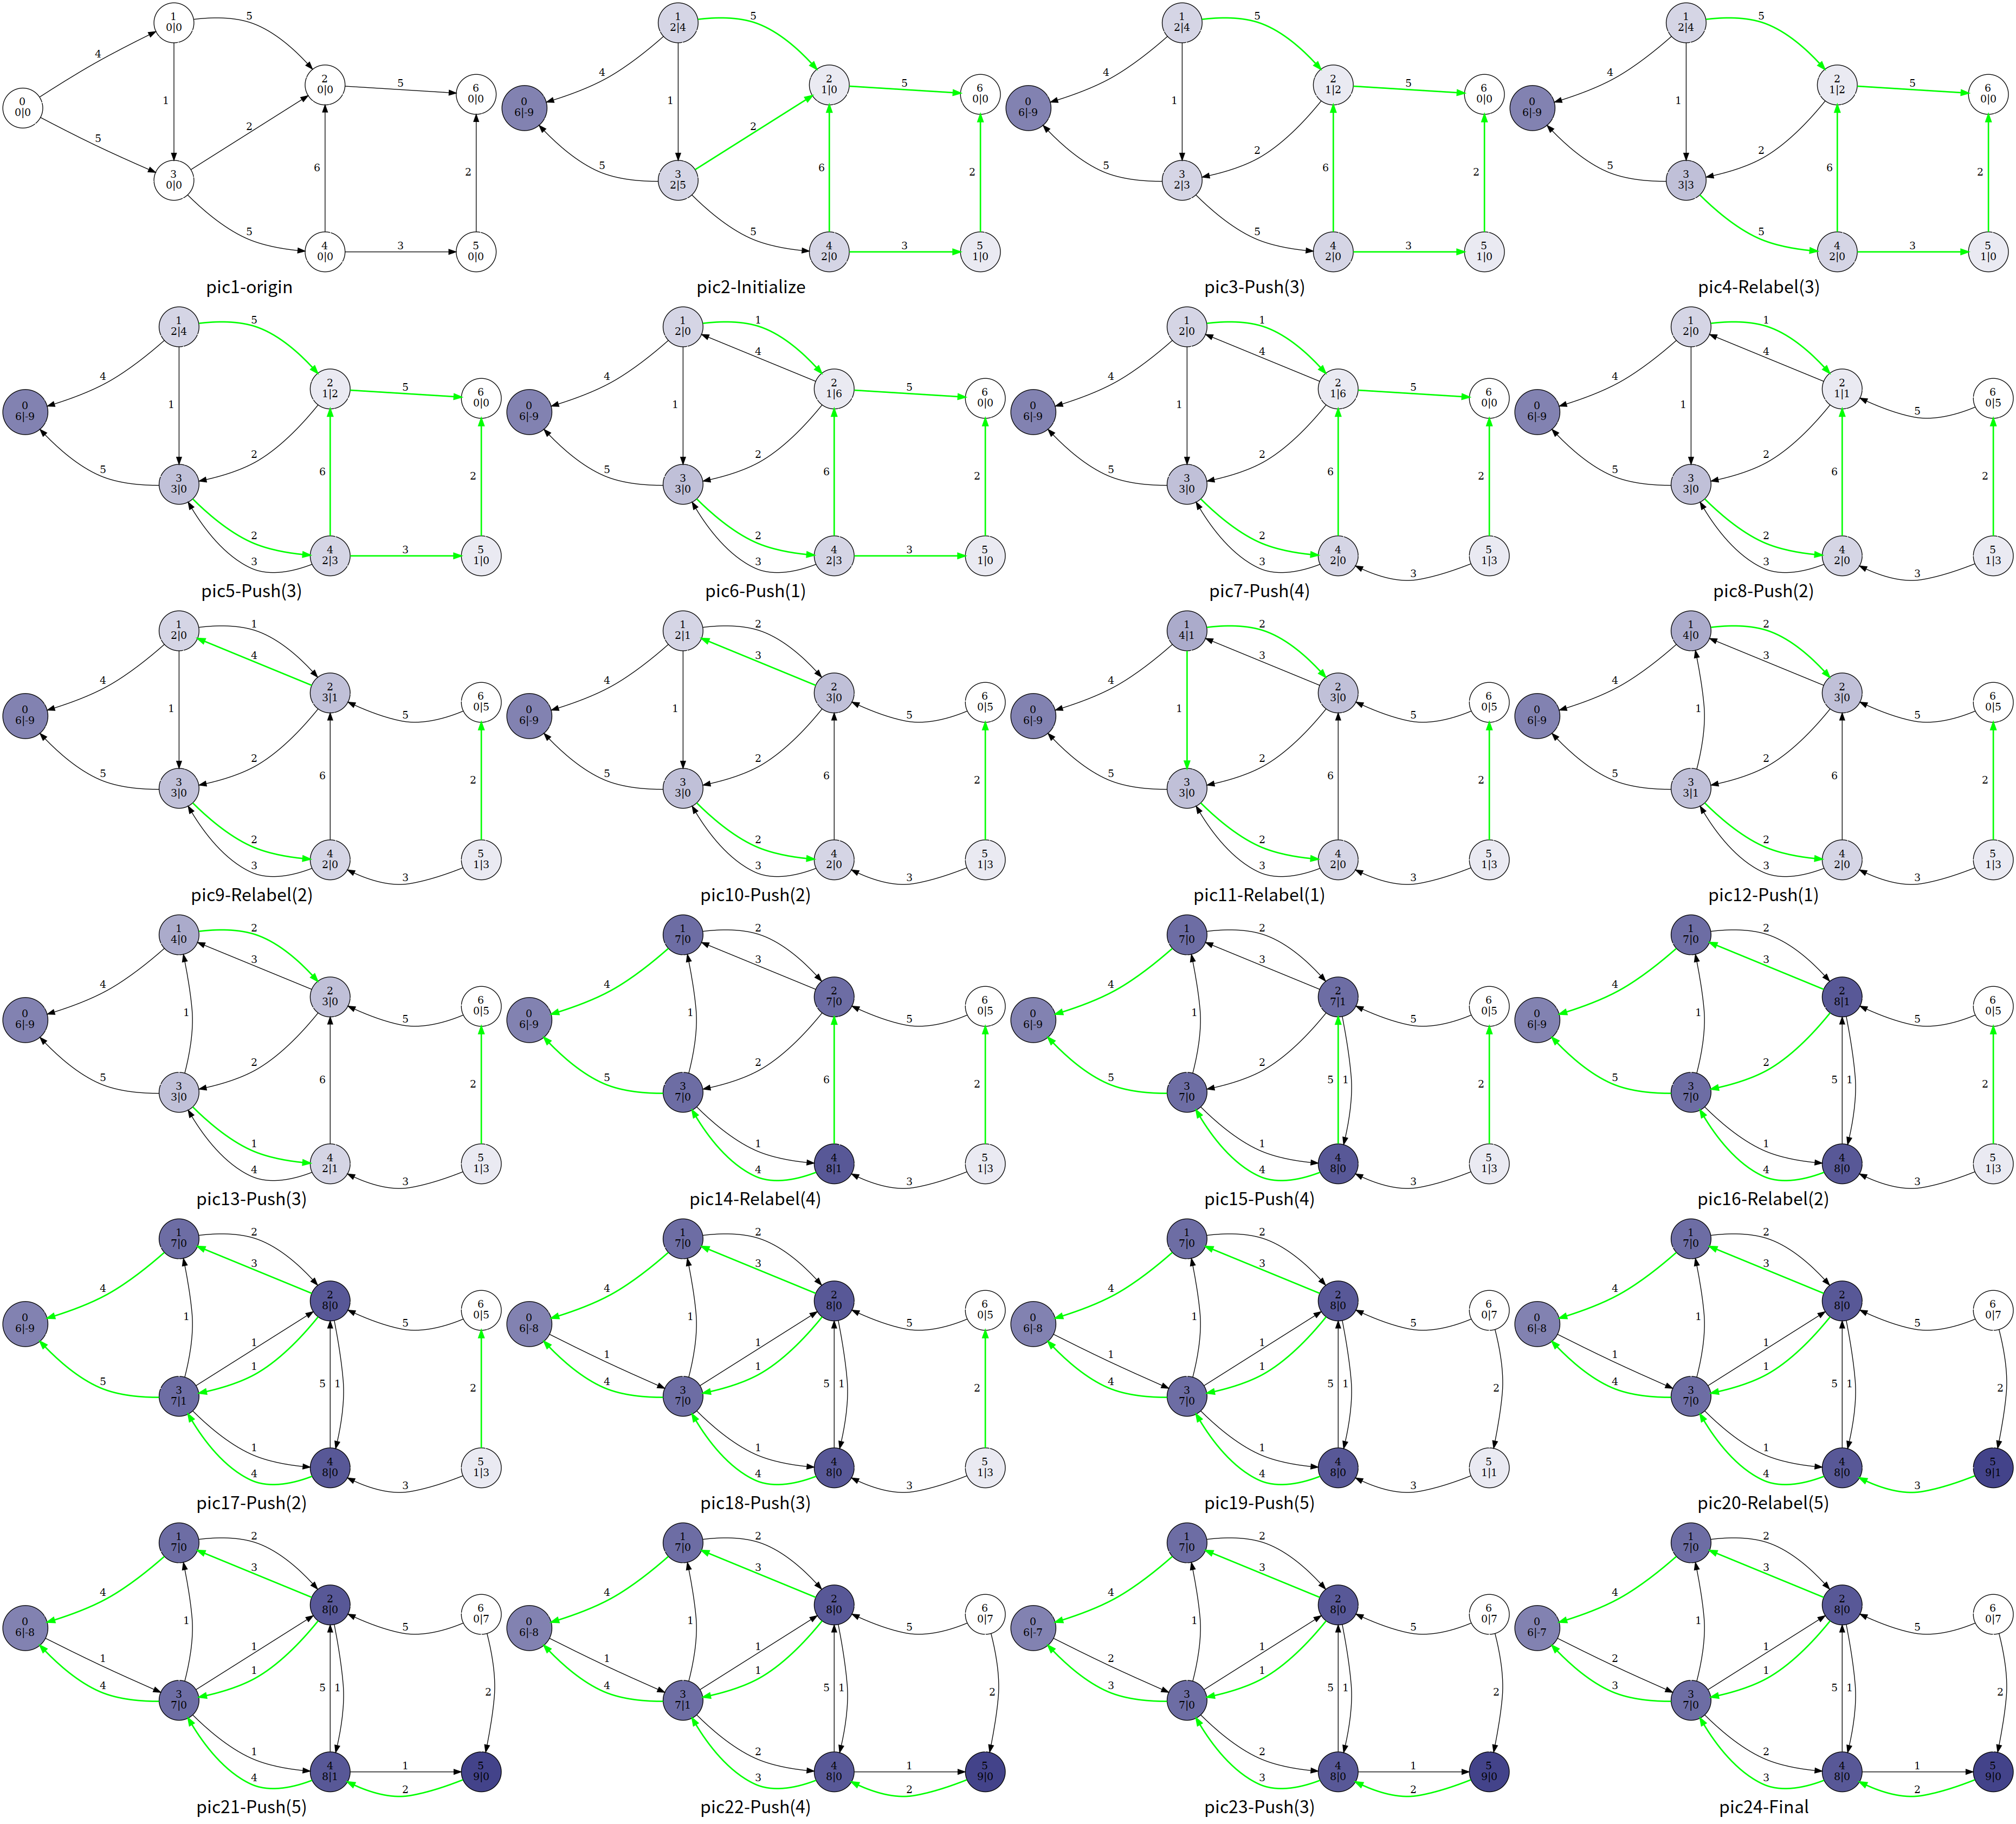
\includegraphics[width=14cm]{hhlp.png}
\end{center}
\begin{lstlisting}[style=cpp]
struct HLPP {
    int n, m = 0, s, t;
    std::vector<edge> e;      // 边 //
    std::vector<node> nd;     // 点 //
    std::vector<int> g[N];    // 点的连边编号 //
    std::priority_queue<node> q;
    std::queue<int> qq;
    bool vis[N];
    int cnt[N];

    void init() {
        e.clear();
        nd.clear();
        for (int i = 0; i <= n + 1; i++) {
            nd.push_back(node(inf, i, 0));
            g[i].clear();
            vis[i] = false;
        }
    }

    void add(int u, int v, LL w) {
        e.push_back(edge(u, v, w));
        e.push_back(edge(v, u, 0));
        g[u].push_back(m++);
        g[v].push_back(m++);
    }

    void bfs() {
        nd[t].hight = 0;
        qq.push(t);
        while (!qq.empty()) {
            int u = qq.front();
            qq.pop();
            vis[u] = false;
            for (auto j : g[u]) {
                int v = e[j].to;
                if (e[j].cap == 0 && nd[v].hight > nd[u].hight + 1) {
                    nd[v].hight = nd[u].hight + 1;
                    if (vis[v] == false) {
                        qq.push(v);
                        vis[v] = true;
                    }
                }
            }
        }
        return;
    }

    void _push(int u) {
        for (auto j : g[u]) {
            edge &ee = e[j], &er = e[j ^ 1];
            int v = ee.to;
            node &nu = nd[u], &nv = nd[v];
            if (ee.cap && nv.hight + 1 == nu.hight) {
                // 推流 //
                LL flow = std::min(ee.cap, nu.flow);
                ee.cap -= flow, er.cap += flow;
                nu.flow -= flow, nv.flow += flow;
                if (vis[v] == false && v != t && v != s) {
                    q.push(nv);
                    vis[v] = true;
                }
                if (nu.flow == 0) break;
            }
        }
    }

    void relabel(int u) {
        nd[u].hight = inf;
        for (auto j : g[u]) {
            int v = e[j].to;
            if (e[j].cap && nd[v].hight + 1 < nd[u].hight) {
                nd[u].hight = nd[v].hight + 1;
            }
        }
    }

    LL hlpp() {
        bfs();
        if (nd[s].hight == inf) return 0;
        nd[s].hight = n;
        for (int i = 1; i <= n; i++) {
            if (nd[i].hight < inf) cnt[nd[i].hight]++;
        }
        for (auto j : g[s]) {
            int v = e[j].to;
            int flow = e[j].cap;
            if (flow) {
                e[j].cap -= flow, e[j ^ 1].cap += flow;
                nd[s].flow -= flow, nd[v].flow += flow;
                if (vis[v] == false && v != s && v != t) {
                    q.push(nd[v]);
                    vis[v] = true;
                }
            }
        }
        while (!q.empty()) {
            int u = q.top().id;
            q.pop();
            vis[u] = false;
            _push(u);
            if (nd[u].flow) {
                cnt[nd[u].hight]--;
                if (cnt[nd[u].hight] == 0) {
                    for (int i = 1; i <= n; i++) {
                        if (i != s && i != t && nd[i].hight > nd[u].hight && nd[i].hight < n + 1) {
                            nd[i].hight = n + 1;
                        }
                    }
                }
                // 上面为 gap 优化 //
                relabel(u);
                cnt[nd[u].hight]++;
                q.push(nd[u]);
                vis[u] = true;
            }
        }
        return nd[t].flow;
    }
} maxf;
\end{lstlisting}

\subsection{ 网络流 - 费用流 }

\subsubsection{ Dinic + SPFA }
处理无负环的网络.
\begin{lstlisting}[style=cpp]
struct edge {
    int from, to;
    LL cap, cost;

    edge(int u, int v, LL c, LL w) : from(u), to(v), cap(c), cost(w) {}
};

struct MCMF {
    int n, m = 0, s, t;
    std::vector<edge> e;
    vi g[N];
    int cur[N], vis[N];
    LL dist[N], minc;

    void init(int n) {
        for (int i = 0; i < n; i++) g[i].clear();
        e.clear();
        minc = m = 0;
    }

    void add(int from, int to, LL cap, LL cost) {
        e.push_back(edge(from, to, cap, cost));
        e.push_back(edge(to, from, 0, -cost));
        g[from].push_back(m++);
        g[to].push_back(m++);
    }

    bool spfa() {
        rep(i, 1, n) { dist[i] = INF, cur[i] = 0; }
        std::queue<int> q;
        q.push(s), dist[s] = 0, vis[s] = 1;
        while (!q.empty()) {
            int u = q.front();
            q.pop();
            vis[u] = 0;
            for (int j = cur[u]; j < g[u].size(); j++) {
                edge& ee = e[g[u][j]];
                int v = ee.to;
                if (ee.cap && dist[v] > dist[u] + ee.cost) {
                    dist[v] = dist[u] + ee.cost;
                    if (!vis[v]) {
                        q.push(v);
                        vis[v] = 1;
                    }
                }
            }
        }
        return dist[t] != INF;
    }

    LL dfs(int u, LL now) {
        if (u == t) return now;
        vis[u] = 1;
        LL ans = 0;
        for (int& i = cur[u]; i < g[u].size() && ans < now; i++) {
            edge &ee = e[g[u][i]], &er = e[g[u][i] ^ 1];
            int v = ee.to;
            if (!vis[v] && ee.cap && dist[v] == dist[u] + ee.cost) {
                LL f = dfs(v, std::min(ee.cap, now - ans));
                if (f) {
                    minc += f * ee.cost, ans += f;
                    ee.cap -= f;
                    er.cap += f;
                }
            }
        }
        vis[u] = 0;
        return ans;
    }

    PLL mcmf() {
        LL maxf = 0;
        while (spfa()) {
            LL tmp;
            while ((tmp = dfs(s, INF))) maxf += tmp;
        }
        return std::makepair(maxf, minc);
    }
} minc_maxf;
\end{lstlisting}

\subsubsection{ Primal-Dual 原始对偶算法 }
处理无负环的网络.
\begin{lstlisting}[style=cpp]
struct edge {
    int from, to;
    LL cap, cost;

    edge(int u, int v, LL c, LL w) : from(u), to(v), cap(c), cost(w) {}
};

struct node {
    int v, e;

    node(int _v = 0, int _e = 0) : v(_v), e(_e) {}
};

const int maxn = 5000 + 10;

struct MCMF {
    int n, m = 0, s, t;
    std::vector<edge> e;
    vi g[maxn];
    int dis[maxn], vis[maxn], h[maxn];
    node p[maxn * 2];

    void add(int from, int to, LL cap, LL cost) {
        e.push_back(edge(from, to, cap, cost));
        e.push_back(edge(to, from, 0, -cost));
        g[from].push_back(m++);
        g[to].push_back(m++);
    }

    bool dijkstra() {
        std::priority_queue<PII, std::vector<PII>, std::greater<PII>> q;
        for (int i = 1; i <= n; i++) {
            dis[i] = inf;
            vis[i] = 0;
        }
        dis[s] = 0;
        q.push({0, s});
        while (!q.empty()) {
            int u = q.top().ss;
            q.pop();
            if (vis[u]) continue;
            vis[u] = 1;
            for (auto i : g[u]) {
                edge ee = e[i];
                int v = ee.to, nc = ee.cost + h[u] - h[v];
                if (ee.cap and dis[v] > dis[u] + nc) {
                    dis[v] = dis[u] + nc;
                    p[v] = node(u, i);
                    if (!vis[v]) q.push({dis[v], v});
                }
            }
        }
        return dis[t] != inf;
    }

    void spfa() {
        std::queue<int> q;
        for (int i = 1; i <= n; i++) h[i] = inf;
        h[s] = 0, vis[s] = 1;
        q.push(s);
        while (!q.empty()) {
            int u = q.front();
            q.pop();
            vis[u] = 0;
            for (auto i : g[u]) {
                edge ee = e[i];
                int v = ee.to;
                if (ee.cap and h[v] > h[u] + ee.cost) {
                    h[v] = h[u] + ee.cost;
                    if (!vis[v]) {
                        vis[v] = 1;
                        q.push(v);
                    }
                }
            }
        }
    }

    PLL mcmf() {
        LL maxf = 0, minc = 0;
        spfa();
        while (dijkstra()) {
            LL minf = INF;
            for (int i = 1; i <= n; i++) h[i] += dis[i];
            for (int i = t; i != s; i = p[i].v) minf = std::min(minf, e[p[i].e].cap);
            for (int i = t; i != s; i = p[i].v) {
                e[p[i].e].cap -= minf;
                e[p[i].e ^ 1].cap += minf;
            }
            maxf += minf;
            minc += minf * h[t];
        }
        return std::makepair(maxf, minc);
    }
} minc_maxf;
\end{lstlisting}

\subsection{ 网络流 - 最小割 }
最小割解决的问题是将图中的点集 $V$ 划分成 $S$ 与 $T$, 使得 $S$ 与 $T$ 之间的连边的容量总和最小. 
\subsubsection{ 最大流最小割定理 }
网络中 $s$  到 $t$ 的最大流流量的值等于所要求的最小割的值. 所以求最小割只需要跑 Dinic 即可. 
\subsubsection{ 获取 $S$ 中的点 }
在 Dinic 的 $\operatorname{bfs}$ 函数中, 每次将所有点的 $d$ 数组值改为无穷大, 最后跑完最大流之后 $d$ 数组不为无穷大的就是和源点一起在 $S$ 集合中的点.  
\subsubsection{ 例子 }
最小割的本质是对图中点集进行 $2$-划分, 网络流只是求解答案的手段. 
\begin{enumerate}
	\item 在图中花费最小的代价断开一些边使得源点 $s$ 无法流到汇点 $t$

    直接跑最大流就得到了答案. 
    
    \item 在图中删除最少的点使得源点 $s$ 无法流到汇点 $t$

    对每个点进行拆点, 在 $i$ 与 $i'$ 之间建立容量为 $1$ 的有向边. 

\end{enumerate}

\subsection{ 图匹配 - 二分图最大匹配 }
\subsubsection{ Kuhn-Munkres 算法 }
时间复杂度: $O(n^3)$.
\begin{lstlisting}[style=cpp]
auto KM = [&](int n1, int n2, vvi e) -> std::pair<vi, vi> {
    vi vis(n2 + 1);
    vi l(n1 + 1, -1), r(n2 + 1, -1);
    std::function<bool(int)> dfs = [&](int u) -> bool {
        for (auto v : e[u]) {
            if (!vis[v]) {
                vis[v] = 1;
                if (r[v] == -1 or dfs(r[v])) {
                    r[v] = u;
                    return true;
                }
            }
        }
        return false;
    };
    for (int i = 1; i <= n1; i++) {
        std::fill(all(vis), 0);
        dfs(i);
    }
    for (int i = 1; i <= n2; i++) {
        if (r[i] == -1) continue;
        l[r[i]] = i;
    }
    return {l, r};
};
auto [mchl, mchr] = KM(n1, n2, e);
std::cout << mchl.size() - std::count(all(mchl), -1) << endl;
\end{lstlisting}

\subsubsection{ Hopcroft-Karp 算法 }
据说时间复杂度是 $O(m \sqrt{n})$ 的, 但是快的飞起. 
\begin{lstlisting}[style=cpp]
vpi e(m);
auto hopcroft_karp = [&](int n, int m, vpi& e) -> std::pair<vi, vi> {
    vi g(e.size()), l(n + 1, -1), r(m + 1, -1), d(n + 2);
    for (auto [u, v] : e) d[u]++;
    std::partial_sum(all(d), d.begin());
    for (auto [u, v] : e) g[--d[u]] = v;
    for (vi a, p, q(n + 1);;) {
        a.assign(n + 1, -1);
        p.assign(n + 1, -1);
        int t = 1;
        for (int i = 1; i <= n; i++) {
            if (l[i] == -1) {
                q[t++] = a[i] = p[i] = i;
            }
        }
        bool match = false;
        for (int i = 1; i < t; i++) {
            int u = q[i];
            if (l[a[u]] != -1) continue;
            for (int j = d[u]; j < d[u + 1]; j++) {
                int v = g[j];
                if (r[v] == -1) {
                    while (v != -1) {
                        r[v] = u;
                        std::swap(l[u], v);
                        u = p[u];
                    }
                    match = true;
                    break;
                }
                if (p[r[v]] == -1) {
                    q[t++] = v = r[v];
                    p[v] = u;
                    a[v] = a[u];
                }
            }
        }
        if (!match) break;
    }
    return {l, r};
};
auto [mchl, mchr] = hopcroft_karp(n1, n2, e);
std::cout << mchl.size() - std::count(all(mchl), -1) << endl;
\end{lstlisting}

\subsection{ 图匹配 - 二分图最大权匹配 }
\subsubsection{Kuhn-Munkres}
注意是否为完美匹配, 非完美选 $0$, 完美选 $-INF$. 
\begin{lstlisting}[style=cpp]
auto KM = [&](int n, vvl e) -> std::tuple<LL, vi, vi> {
    vl la(n + 1), lb(n + 1), pp(n + 1), vx(n + 1);
    vi l(n + 1, -1), r(n + 1, -1);
    vi va(n + 1), vb(n + 1);
    LL delta;
    auto bfs = [&](int x) -> void {
        int a, y = 0, y1 = 0;
        std::fill(all(pp), 0);
        std::fill(all(vx), INF);
        r[y] = x;
        do {
            a = r[y], delta = INF, vb[y] = 1;
            for (int b = 1; b <= n; b++) {
                if (!vb[b]) {
                    if (vx[b] > la[a] + lb[b] - e[a][b]) {
                        vx[b] = la[a] + lb[b] - e[a][b];
                        pp[b] = y;
                    }
                    if (vx[b] < delta) {
                        delta = vx[b];
                        y1 = b;
                    }
                }
            }
            for (int b = 0; b <= n; b++) {
                if (vb[b]) {
                    la[r[b]] -= delta;
                    lb[b] += delta;
                } else
                    vx[b] -= delta;
            }
            y = y1;
        } while (r[y] != -1);
        while (y) {
            r[y] = r[pp[y]];
            y = pp[y];
        }
    };
    for (int i = 1; i <= n; i++) {
        std::fill(all(vb), 0);
        bfs(i);
    }
    LL ans = 0;
    for (int i = 1; i <= n; i++) {
        if (r[i] == -1) continue;
        l[r[i]] = i;
        ans += e[r[i]][i];
    }
    return {ans, l, r};
};

auto [ans, mchl, mchr] = KM(n, e);
\end{lstlisting}


\newpage
\section{ 计算几何 }
\subsection{ 二维基础 }
\subsubsection{ 向量计算 }
\begin{lstlisting}[style=cpp]
tandu struct pnt {
    T x, y;

    pnt(T _x = 0, T _y = 0) { x = _x, y = _y; }

    pnt operator+(const pnt& a) const { return pnt(x + a.x, y + a.y); }

    pnt operator-(const pnt& a) const { return pnt(x - a.x, y - a.y); }

    /*
    bool operator<(const pnt& a) const {
        if (std::is_same<T, double>::value) {
            if (fabs(x - a.x) < eps) return y < a.y;
        } else {
            if (x == a.x) return y < a.y;
        }
        return x < a.x;
    }
    */

    // 注意数乘会不会爆 int //
    pnt operator*(const T k) const { return pnt(k * x, k * y); }

    U operator*(const pnt& a) const { return (U) x * a.x + (U) y * a.y; }

    U operator^(const pnt& a) const { return (U) x * a.y - (U) y * a.x; }

    U dist(const pnt a) { return ((U) a.x - x) * ((U) a.x - x) + ((U) a.y - y) * ((U) a.y - y); }

    U len() { return dist(pnt(0, 0)); }

    // a, b, c 成逆时针 //
    friend U area(pnt a, pnt b, pnt c) { return (b - a) ^ (c - a); }

    // 两向量夹角,返回 cos 值 //
    double get_angle(pnt a) {
        return (double) (pnt(x, y) * a) / sqrt((double) pnt(x, y).len() * (double) a.len());
    }
};
typedef pnt<LL, LL> point;
\end{lstlisting}

\subsubsection{ 线段 }
\begin{lstlisting}
struct line {
    point a, b;

    line(point _a = {}, point _b = {}) { a = _a, b = _b; }

    // 交点类型为 double //
    friend point iPoint(line p, line q) {
        point v1 = p.b - p.a;
        point v2 = q.b - q.a;
        point u = q.a - p.a;
        return q.a + (q.b - q.a) * ((u ^ v1) * 1. / (v1 ^ v2));
    }

    // 极角排序 //
    bool operator<(const line& p) const {
        double t1 = std::atan2((b - a).y, (b - a).x);
        double t2 = std::atan2((p.b - p.a).y, (p.b - p.a).x);
        if (fabs(t1 - t2) > eps) {
            return t1 < t2;
        }
        return ((p.a - a) ^ (p.b - a)) > eps;
    }
};
\end{lstlisting}

\subsection{ 凸包 }
\subsubsection{ 二维凸包 }
\begin{lstlisting}
// convex hull //
auto andrew = [&]() -> std::vector<point> {
    std::sort(all(v));
    std::vector<point> stk;
    for (int i = 0; i < n; i++) {
        point x = v[i];
        while (stk.size() > 1 and ((stk.end()[-1] - stk.end()[-2]) ^ (x - stk.end()[-2])) <= 0) {
            stk.pop_back();
        }
        stk.push_back(x);
    }
    int tmp = stk.size();
    for (int i = n - 2; i >= 0; i--) {
        point x = v[i];
        while (stk.size() > tmp and ((stk.end()[-1] - stk.end()[-2]) ^ (x - stk.end()[-2])) <= 0) {
            stk.pop_back();
        }
        stk.push_back(x);
    }
    return stk;
};
auto convex = andrew();
\end{lstlisting}

\subsection{ 半平面交 }
\begin{lstlisting}
// half plain intersection //
auto halfPlain = [&](std::vector<line>& ln) -> std::vector<point> {
    std::sort(all(ln));
    ln.erase(
        unique(
            all(ln),
            [](line& p, line& q) {
                double t1 = std::atan2((p.b - p.a).y, (p.b - p.a).x);
                double t2 = std::atan2((q.b - q.a).y, (q.b - q.a).x);
                return fabs((t1 - t2)) < eps;
            }),
        ln.end());
    auto check = [&](line p, line q, line r) -> bool {
        point a = iPoint(p, q);
        return ((r.b - r.a) ^ (a - r.a)) < -eps;
    };
    line q[ln.size() + 2];
    int hh = 1, tt = 0;
    q[++tt] = ln[0];
    q[++tt] = ln[1];
    for (int i = 2; i < (int) ln.size(); i++) {
        while (hh < tt and check(q[tt - 1], q[tt], ln[i])) tt--;
        while (hh < tt and check(q[hh + 1], q[hh], ln[i])) hh++;
        q[++tt] = ln[i];
    }
    while (hh < tt and check(q[tt - 1], q[tt], q[hh])) tt--;
    while (hh < tt and check(q[hh + 1], q[hh], q[tt])) hh++;
    q[tt + 1] = q[hh];
    std::vector<point> ans;
    for (int i = hh; i <= tt; i++) {
        ans.push_back(iPoint(q[i], q[i + 1]));
    }
    return ans;
};
auto p = halfPlain(ln);
\end{lstlisting}

\newpage
\section{离线算法}

\subsection{ 莫队 }
\subsubsection{ 普通莫队 }
\begin{lstlisting}
int block = n / sqrt(2 * m / 3);
std::sort(all(q), [&](node a, node b) {
    return a.l / block == b.l / block ? (a.r == b.r ? 0 : ((a.l / block) & 1) ^ (a.r < b.r))
                                      : a.l < b.l;
});

auto move = [&](int x, int op) -> void {
    if (op == 1) {
        ...
    } else {
        ...
    }
};

for (int k = 1, l = 1, r = 0; k <= m; k++) {
    node Q = q[k];
    while (l > Q.l) {
        move(--l, 1);
    }
    while (r < Q.r) {
        move(++r, 1);
    }
    while (l < Q.l) {
        move(l++, -1);
    }
    while (r > Q.r) {
        move(r--, -1);
    }
}
\end{lstlisting}

\subsubsection{ 带修改莫队 }

\subsubsection{ 树上莫队 }

\subsection{ 离散化 }
\begin{lstlisting}
std::sort(all(a));
a.erase(unique(all(a)), a.end());
auto get_id = [&](const int& x) -> int { return lower_bound(all(a), x) - a.begin() + 1; };
\end{lstlisting}

\subsection{ CDQ 分治 }
$n$ 个三维数对 $(a_i, b_i, c_i)$, 设 $f(i)$ 表示 $a_j \leqslant a_i$ 且 $b_j \leqslant b_i$ 且  $c_j \leqslant c_i$ 且 $i \neq j$ 的个数. 

输出 $f(i) \ (0 \leqslant i \leqslant n - 1)$  的值.
\begin{lstlisting}[style=cpp]
// 洛谷 P3810 【模板】三维偏序( 陌上花开 )

struct data {
    int a, b, c, cnt, ans;

    data(int _a = 0, int _b = 0, int _c = 0, int _cnt = 0, int _ans = 0) {
        a = _a, b = _b, c = _c, cnt = _cnt, ans = _ans;
    }

    bool operator!=(data x) {
        if (a != x.a) return true;
        if (b != x.b) return true;
        if (c != x.c) return true;
        return false;
    }
};

int main() {
    std::ios::sync_with_stdio(false);
    std::cin.tie(0);
    std::cout.tie(0);

    int n, k;
    std::cin >> n >> k;
    static data v1[N], v2[N];
    for (int i = 1; i <= n; i++) {
        std::cin >> v1[i].a >> v1[i].b >> v1[i].c;
    }

    std::sort(v1 + 1, v1 + n + 1, [&](data x, data y) {
        if (x.a != y.a) return x.a < y.a;
        if (x.b != y.b) return x.b < y.b;
        return x.c < y.c;
    });

    int t = 0, top = 0;
    for (int i = 1; i <= n; i++) {
        t++;
        if (v1[i] != v1[i + 1]) {
            v2[++top] = v1[i];
            v2[top].cnt = t;
            t = 0;
        }
    }

    // BIT //
    
    // CDQ //
    std::function<void(int, int)> CDQ = [&](int l, int r) -> void {
        if (l == r) return;
        int mid = (l + r) >> 1;
        CDQ(l, mid), CDQ(mid + 1, r);
        std::sort(v2 + l, v2 + mid + 1, [&](data x, data y) {
            if (x.b != y.b) return x.b < y.b;
            return x.c < y.c;
        });
        std::sort(v2 + mid + 1, v2 + r + 1, [&](data x, data y) {
            if (x.b != y.b) return x.b < y.b;
            return x.c < y.c;
        });
        int i = l, j = mid + 1;
        while (j <= r) {
            while (i <= mid && v2[i].b <= v2[j].b) {
                add(v2[i].c, v2[i].cnt);
                i++;
            }
            v2[j].ans += query(v2[j].c);
            j++;
        }
        for (int ii = l; ii < i; ii++) {
            add(v2[ii].c, -v2[ii].cnt);
        }
        return;
    };

    CDQ(1, top);
    vi ans(n + 1);
    for (int i = 1; i <= top; i++) {
        ans[v2[i].ans + v2[i].cnt] += v2[i].cnt;
    }
    for (int i = 1; i <= n; i++) {
        std::cout << ans[i] << endl;
    }

    return 0;
}
\end{lstlisting}

\end{document}